\documentclass[journal]{IEEEtran}
\ifCLASSINFOpdf
\else
\fi
\hyphenation{op-tical net-works semi-conduc-tor}
\usepackage{graphicx}
\usepackage{tabularx}
\usepackage{booktabs} % Package for professional-looking tables
\usepackage{siunitx}
\usepackage{makecell}
\usepackage[T1]{fontenc}
\usepackage{multirow}
\usepackage{hyperref}
\sisetup{group-digits=false, detect-weight, mode=text} % Settings for siunitx: disable digit grouping, detect font weight, use text mode


\begin{document}

\title{BioMark: Biomarker Analysis Tool}

\author{Mehmet Ali Balikci\IEEEauthorrefmark{1}, Cyrille Njume Mesue\IEEEauthorrefmark{1}, Ali Cakmak\IEEEauthorrefmark{1}*

\thanks{\IEEEauthorrefmark{1}Istanbul Technical University, Ayazaga Campus, Maslak 34469 Istanbul, Turkey}
\thanks{*\textbf{Corresponding author:} Ali Cakmak, ali.cakmak@itu.edu.tr}
}


% Paper headers
\markboth{Journal of \LaTeX\ Class Files}%
{Balikci \MakeLowercase{\textit{et al.}}: Bare Demo of IEEEtran.cls for IEEE Journals}

% Make the title area
\maketitle

% Abstract and keywords
\IEEEtitleabstractindextext{%
\begin{abstract}
Biomarkers play a pivotal role in disease diagnosis and prognosis by offering molecular insights into biological states. The rapid growth of high-throughput omics technologies has enabled the generation of large-scale biomarker datasets, yet analyzing these complex, high-dimensional data remains a major challenge—particularly for researchers lacking advanced computational expertise. While numerous tools exist for omics data analysis, many fall short in providing an integrated, user-friendly environment tailored specifically for biomarker discovery and interpretation.

To address this gap, we present BioMark, a web-based platform designed to streamline biomarker analysis across diverse omics types. BioMark integrates robust statistical methods with widely used machine learning algorithms to support key workflows including differential analysis, clustering, and classification. The platform emphasizes accessibility, offering intuitive visualizations and automated reporting to facilitate interpretation and dissemination of results. Notably, BioMark also offers a feature-ranking strategy that consolidates outputs from multiple analytical methods, enhancing the robustness of biomarker identification. By lowering the barrier to advanced biomarker analytics, BioMark empowers a broader range of researchers to uncover clinically relevant molecular signatures and accelerate translational research. Biomark is available online at \href{https://bioinf.itu.edu.tr/biomark}{https://bioinf.itu.edu.tr/biomark}.
\end{abstract}

% Keywords for the paper
\begin{IEEEkeywords}

disease diagnosis, biomarker discovery, artificial intelligence, multivariate analysis
\end{IEEEkeywords}}

% Display abstract and keywords for non-conference mode
\IEEEdisplaynontitleabstractindextext
% This command has no effect when using compsoc under a non-conference mode.


% Extra information for peer review papers
\IEEEpeerreviewmaketitle

\section{Introduction}

\IEEEPARstart{B}{iomarkers} are useful to diagnose diseases and monitor the prognosis of patients. These molecular indicators provide critical insights into biological states, aiding in the identification of disease presence and the prediction of disease trajectory and outcome \cite{Zheng2020_CancerReview}. Biomarkers encompass a wide range of molecular entities, such as genomic alterations, gene expression levels (transcriptomics), protein abundance (proteomics), and metabolite concentrations (metabolomics), and they are fundamental to understanding the molecular underpinnings of health and disease. Their accurate identification and interpretation across diverse biological contexts are paramount for improving diagnostic capabilities, monitoring disease progression, predicting treatment responses, and ultimately personalizing treatment strategies in various medical conditions.

The advent of high-throughput technologies has led to an exponential increase in the volume and complexity of biomarker data. These technologies, including next-generation sequencing, microarray analysis, and advanced mass spectrometry, generate vast datasets that often characterize thousands or even millions of molecular features simultaneously \cite{MetaboAnalyst_2009, MetaboAnalystR_2018, MetaboLink_2024, WebSpecmine_2019, MOMIC_2022, Gruca2022_MAINE, Lu2024_GenoCraft, MiBiOmics_2021}. Analyzing these large, heterogeneous, and intricate datasets presents significant computational challenges. Issues such as data noise, missing values, batch effects, high dimensionality (where the number of features far exceeds the number of samples), and the need for integrating data from multiple omics layers require sophisticated computational, statistical, and machine learning methods for effective analysis \cite{MOMIC_2022}, \cite{Multiomix_2022}, \cite{exploRase_2006}. For many researchers and clinicians, who may not possess extensive programming skills or have access to dedicated bioinformatics support and powerful computational resources, applying these advanced analytical methods remains a considerable barrier \cite{exploRase_2006}, \cite{XCMSOnline_2012}.

To address these challenges, a diverse landscape of computational tools has been developed. Many platforms offer comprehensive suites for general omics analysis, including data processing, statistical tests, and visualization, often delivered via accessible web interfaces to support researchers without extensive programming backgrounds \cite{Akhmedov2020_OmicsPlayground, Gruca2022_MAINE, Lu2024_GenoCraft, MetaboAnalyst_2009, WebSpecmine_2019}. Examples range from broad platforms like \textbf{OmicsAnalyst} \cite{OmicsAnalyst_2021} and \textbf{PROMO} \cite{Netanely2019_PROMO} to more specialized resources for metabolomics like \textbf{Metabolomics Workbench} \cite{MetabolomicsWorkbench_2016} and \textbf{iMAP} \cite{iMAP_2021}. Other tools focus on specific functionalities such as multi-omics integration \cite{MOMIC_2022}, cancer prognosis analysis \cite{Zheng2020_CancerReview, OSacc_2019}, or pathway informatics using databases like KEGG \cite{KEGG_2017} and Reactome \cite{Reactome_2020}. Despite this rich ecosystem, a critical gap remains. Many existing tools have limitations in their ease of use for non-experts, the breadth of integrated analytical methods, or the intuitive visualization of results, forcing researchers to use multiple, disconnected tools for a complete analysis \cite{exploRase_2006, XCMSOnline_2012}. There is a persistent need for a platform that seamlessly integrates the essential biomarker analysis workflows—identifying significant differences, discovering patient subgroups, and building predictive models—into a single, cohesive environment.

In response to this need, we have developed BioMark, a novel web-based tool designed to provide a user-friendly and comprehensive platform for biomarker data analysis. BioMark enables researchers to upload their high-dimensional biomarker datasets and perform crucial analyses including clustering analysis to discover hidden patient subgroups, and classification analysis to build predictive models for diagnosis and prognosis. The tool employs a combination of robust statistical methods and widely-used machine learning techniques, and provides intuitive visualizations to aid in the interpretation of complex results. Furthermore, BioMark offers a unique capability to combine and rank biomarker lists obtained from different analytical methods used in differential analysis, providing a more robust identification of important features by consolidating results from various perspectives. BioMark aims to make advanced biomarker analysis accessible to a wider audience, facilitating the identification of biomarkers useful for disease diagnosis and prognosis and accelerating research in these areas, with the capability to generate comprehensive reports summarizing the analysis findings and visualizations for easy dissemination of results.

To demonstrate its practical utility, we apply BioMark to real-world transcriptomics datasets from prostate and breast cancer studies. These case studies showcase the platform's effectiveness in identifying significant biomarkers, revealing patient subgroups through clustering, and constructing accurate diagnostic models. The remainder of this paper is organized as follows: Section II reviews related work, Section III details the architecture and methodologies of BioMark, Section IV presents the performance evaluation and case study results, and Section V provides concluding remarks.

\section{RELATED WORK}
The increasing availability of high-dimensional omics and biomarker data has led to the development of numerous computational tools and platforms designed to assist researchers in data analysis and interpretation. These tools can be broadly categorized under three umbrella groups: (i) comprehensive analysis platforms, (ii) niche specialized applications, and (iii) resources for downstream biological interpretation. Positioning BioMark within this landscape requires an examination of their respective strengths and limitations.

Comprehensive web-based platforms represent the most common category, offering end-to-end analysis workflows. For instance, \textbf{MetaboAnalyst} \cite{MetaboAnalyst_2009}, \textbf{MetaboAnalystR} \cite{MetaboAnalystR_2018} and \textbf{OmicsAnalyst} \cite{OmicsAnalyst_2021} provide a powerful suite of tools for statistical analysis, functional enrichment, and visualization, but are primarily tailored for metabolomics and multi-omics data integration, respectively. Platforms like \textbf{Omics Playground} \cite{Akhmedov2020_OmicsPlayground} and \textbf{GenoCraft} \cite{Lu2024_GenoCraft} excel in providing interactive and user-friendly interfaces for exploratory data analysis, including dimensionality reduction and clustering. However, a common limitation of these general-purpose tools is that their biomarker discovery workflows often rely on individual statistical methods. While powerful, they typically lack an integrated mechanism to consolidate feature importance rankings from multiple, methodologically distinct approaches (e.g., combining statistical significance from ANOVA with model-based importance from SHAP). This consolidation is a core feature of BioMark, designed to enhance the robustness and reliability of identified biomarker signatures.

A second category consists of specialized tools designed for specific research questions or data types. Numerous web servers, such as \textbf{OSacc} \cite{OSacc_2019}, \textbf{OSuvm} \cite{OSuvm_2020}, and others focusing on specific cancers \cite{OSblca_2019, OSpaad_2020, OSlgg_2020, OSlihc_2020}, are dedicated to survival and prognosis analysis, often using pre-existing public datasets like The Cancer Genome Atlas (TCGA). While invaluable for prognostic studies, these tools are not designed for users to upload and analyze their own datasets for differential expression or classification model building, which is a primary function of BioMark. Other specialized resources focus on advanced visualization (e.g., \textbf{MicrobioSee} \cite{MicrobioSee_2022}), complex multi-omics integration pipelines (e.g., \textbf{MOMIC} \cite{MOMIC_2022}), or specific methods for outcome prediction (e.g., \textbf{X-Tile} \cite{Camp2004_XTile}).

Finally, foundational bioinformatics resources like \textbf{KEGG} \cite{KEGG_2017}, \textbf{Reactome} \cite{Reactome_2020}, and \textbf{Pathway Tools} \cite{PathwayTools_2009} provide the essential pathway and genome informatics necessary for the biological interpretation of results. While indispensable for downstream analysis, these are databases and toolkits rather than platforms for upstream statistical discovery from user-supplied data matrices.

While this diverse landscape offers powerful capabilities, a clear gap remains. Researchers often face a trade-off: either use a general-purpose platform that may lack dedicated, robust biomarker discovery workflows, or piece together multiple specialized tools, which can be inefficient and requires significant bioinformatics expertise. BioMark addresses this gap by providing a single, cohesive web platform specifically architected for biomarker discovery. It uniquely integrates three critical, yet often separate, workflows: (i) robust differential analysis featuring an integrated multi-method feature ranking system to increase confidence in results, (ii) intuitive clustering for sample stratification, and (iii) comprehensive classification model building and evaluation. By focusing on this core biomarker analysis pipeline and prioritizing an intuitive user experience, BioMark empowers researchers without extensive computational backgrounds to perform end-to-end analyses, from raw data to validated biomarker lists and high-performance predictive models.

\section{METHODS}
The BioMark tool is designed as a web-based platform to facilitate the analysis and visualization of biomarker data, primarily focusing on high-dimensional datasets such as gene expression and protein levels. The tool's architecture and functionalities are structured to enable researchers, including those without extensive programming backgrounds, to easily perform advanced analyses and gain meaningful biological insights

\subsection{Architecture}
The BioMark web tool operates through a client-server architecture, as illustrated in Fig.~\ref{fig:architecture}. Users interact with the platform through a web browser, which serves as the client interface. Data and analysis requests selected by the user are sent from the web browser to a back-end system running on a server. This back-end system is responsible for triggering specific analysis programs based on the received requests. These analysis programs process the data, perform necessary computations, and perform statistical analyses or machine learning models. Upon completion of the analysis, the generated results, including graphs, tables, and key findings, are sent back from the back-end system to the user's web browser for display. This architecture ensures that computationally intensive tasks are handled at the server side, providing a responsive user experience through the web interface.

\begin{figure}[htbp]
\centering
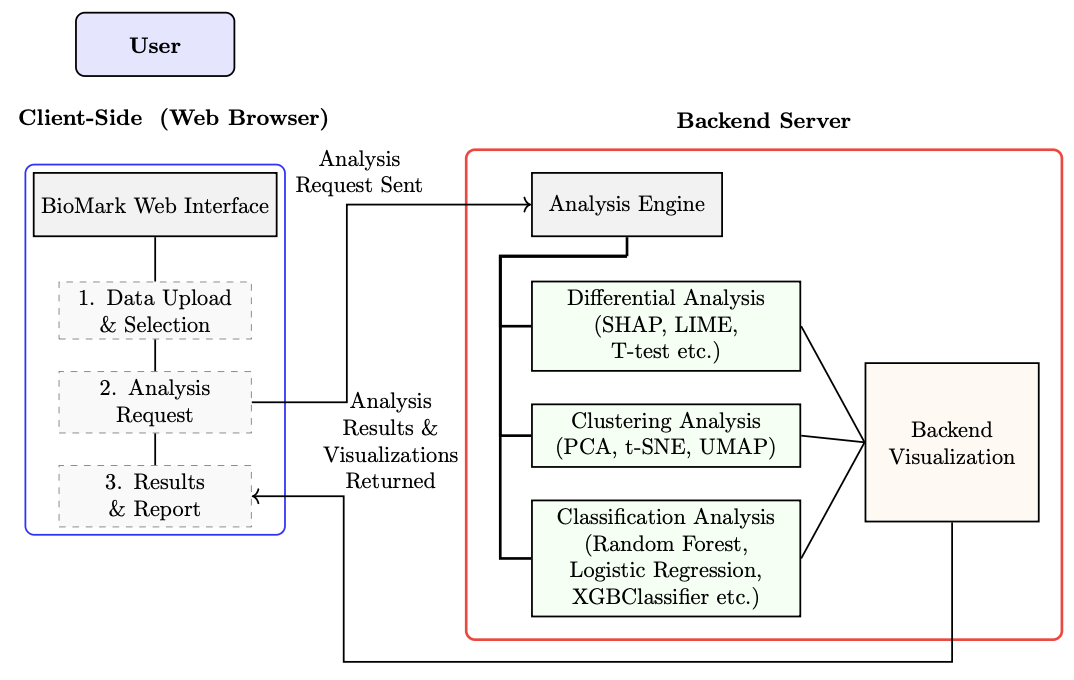
\includegraphics[width=\columnwidth]{architecture_diagram.png}
\caption{The BioMark client-server architecture. Users interact via the web interface to upload data and request analyses. The backend server processes these requests, performs analyses, and returns results and visualizations to the user.}
\label{fig:architecture}
\end{figure}

\subsection{Data Uploading}
The BioMark tool is designed to work with omics datasets, typically in a tabular format where rows represent samples (e.g., patients or experiments) and columns represent biological entities (e.g., genes, proteins, metabolites) or sample metadata (e.g., disease status, sample ID). The primary data format supported for uploading datasets is CSV (Comma Separated Values). The platform also supports compressed files with a .gz extension. Users can upload their own datasets through the web interface. For users new to the platform or wishing to explore its functionalities, a pre-loaded demo dataset is also available and can be downloaded. The tool is optimized to handle high-dimensional data, often characterized by a large number of biomarkers (columns) relative to the number of samples (rows). While primarily focused on numerical data (such as expression levels or concentrations), the tool can also handle categorical columns, particularly for the target variable.

\subsection{Selecting Patient Groups}
The analysis often involves comparing or grouping samples based on specific criteria. BioMark allows for the selection of different classes within a target variable, such as disease status (e.g., healthy vs. diseased). The platform can automatically detect different classes present in the uploaded target variable column, and users can then select the specific classes they wish to include in their analysis. This functionality is particularly important for differential analysis and classification tasks where distinct groups of samples need to be defined.

\subsection{Determining Analysis Groups}
Following the selection of patient groups based on class labels, BioMark allows for determining the specific groups to be compared in the analysis. This step is integral to differential analysis, where the tool aims to find statistically significant differences in biomarker levels between predefined groups (e.g., comparing biomarker profiles of a 'patient' group against a 'healthy' group). The tool is designed to facilitate the comparison between different combinations of selected classes, enabling researchers to explore various group comparisons relevant to their study.

\subsection{Selecting an Analysis Type and Customization}
BioMark offers multiple analysis options to explore and interpret biomarker data. Users can select from core analysis types, including Differential Analysis, Clustering Analysis, and Classification Analysis.
\begin{itemize}
\item \textbf{Differential Analysis:} Aims to identify statistically significant differences in biomarker abundance or activity between predefined groups of samples. This analysis utilizes both traditional statistical tests (such as t-tests and ANOVA, which can be employed by the background modules) and machine learning-based methods (particularly gradient boosting models like CatBoost) to determine group differences and their significance. Feature interpretability techniques like SHAP (SHapley Additive exPlanations) \cite{Lundberg2017_SHAP, Lundberg2020_TreeSHAP} and LIME (Local Interpretable Model-agnostic Explanations) \cite{Ribeiro2016_LIME} are applied to explain which biomarkers are most effective in distinguishing groups and to interpret model results. The feature rankings provided by different methods can be combined to identify the most important biomarkers. This analysis can be performed separately for different pairs of classes.
\item \textbf{Clustering Analysis:} Used to explore how samples naturally group together based on their biomarker profiles without prior group information. Dimension reduction techniques like PCA (Principal Component Analysis), t-SNE (t-Distributed Stochastic Neighbor Embedding), and UMAP (Uniform Manifold Approximation and Projection) are used to visualize data in a lower-dimensional space (2D or 3D), revealing potential subgroups or patterns.
\item \textbf{Classification Analysis:} Focuses on building predictive models that assign samples to specific categories (e.g., disease type) using biomarker data. Machine learning models, e.g., XGBoost, Logistic Regression, etc., are trained for this purpose. Model performance can be evaluated using various metrics (such as F1 score and accuracy) and cross-validation. 
\end{itemize}
BioMark provides options for users to either utilize default parameters for these analyses or to customize detailed parameter settings for more advanced control (such as test dataset size, cross-validation folds, and model tuning options).

\subsubsection{Feature Selection and Workflow Stages}\label{sec:feature_selection_mechanism_label}
BioMark incorporates a robust feature selection mechanism crucial for enhancing the interpretability and performance of downstream analyses, particularly for high-dimensional omics data. This process allows researchers to focus on the most informative biomarkers by reducing noise and computational complexity. The platform distinguishes between two primary analytical stages based on feature selection: "Without Feature Selection" and "After Feature Selection."

\textbf{Feature Selection Mechanism:}
The core feature selection process is initiated immediately following the differential analysis. The \texttt{DifferentiatingFactorAnalysis} module computes feature importance scores for each pair of classes using various methods such as SHAP, ANOVA, T-test, XGBoost Feature Importance, Random Forest Feature Importance, and Permutation Feature Importance. These individual method-specific scores are then consolidated to generate a robust overall feature ranking. For each biomarker, its rank from each method's importance list is summed to create an "overall score." Biomarkers are then sorted by this overall score (lower score indicating higher importance), and the top N features are selected. By default, BioMark selects the top 20 features, but this number can be dynamically adjusted by the user via configurable parameters. This multi-method aggregation strategy enhances the confidence in the identified top features, as they are consistently deemed important across different analytical perspectives.

\textbf{"Without Feature Selection" Stage:}
In this initial stage, all analyses, including preliminary visualizations and classification model training, are performed using the entire high-dimensional dataset with all available features. Results from this stage represent a baseline performance reference before any dimensionality reduction based on feature importance is applied, and corresponding figures are often explicitly labeled "Without Feature Selection."

\textbf{"After Feature Selection" Stage:}
Following the feature selection process, a refined dataset is created by retaining only the top N selected biomarkers (as determined by the aggregated ranking) along with the target class column. All subsequent analyses, including advanced dimensionality reduction visualizations (e.g., PCA, t-SNE, UMAP plots) and re-training of classification models, are then performed exclusively on this reduced, most informative feature set. Results and figures generated in this stage are explicitly labeled with "After Feature Selection," showcasing the enhanced insights and improved model performance achieved by focusing on the most relevant molecular signatures. This two-stage approach allows for a direct comparison of analytical outcomes, emphasizing the value of feature selection in biomarker discovery.

\subsection{Explainability: Visualizing Biomarkers}
Visualizations are a key component of the BioMark tool, enabling users to intuitively explore and interpret their biomarker data and analysis results. The platform generates various types of plots tailored to the specific analyses performed:
\begin{itemize}
\item \textbf{Heatmap:} Displays the levels of important biomarkers across different samples using color intensity, revealing patterns and groupings. Heatmaps can also show comparative feature rankings from different statistical methods in summary analysis.
\item \textbf{PCA Plot:} Visualizes how samples are distributed and clustered in a selected lower-dimensional space (2D or 3D) after PCA dimension reduction.
\item \textbf{t-SNE Plot:} Similar to PCA plots, this visualizes sample distribution and clustering in a selected lower-dimensional space (2D or 3D) after t-SNE dimension reduction.
\item \textbf{SHAP Summary Plot:} From SHAP analysis, this plot shows the overall impact of each feature on the model output and the direction of the effect (positive/negative).
\item \textbf{SHAP Dependence Plot:} Illustrates how the model output changes as the value of a specific feature changes.
\item \textbf{LIME Explanation Plots:} Provide local feature importances that explain the prediction for a single sample based on LIME analysis.
\item \textbf{Statistical Method Summary Plot:} Creates a plot summarizing the results of different statistical methods used in differential analysis, showing comparative feature rankings. Separate summaries can be generated for different pairs of classes.
\end{itemize}

\subsection{Combining and Ranking Multi-Analysis Results}
A significant challenge in biomarker discovery is that different analytical methods—each with its own statistical assumptions and biases—often yield distinct lists of candidate biomarkers. Relying on a single method can lead to findings that are not robust. To address this, BioMark incorporates a powerful feature to consolidate and rank biomarker lists generated from multiple analytical approaches, providing a more reliable, consensus-based result.

The core of this consolidation is a rank aggregation methodology. After differential analysis is performed using various methods (e.g., ANOVA, t-test, SHAP, Random Forest feature importance), BioMark assigns a numerical rank to each biomarker based on its importance score within each method (where rank 1 is the most important). To generate a unified, overall ranking, the platform calculates a "Total Rank Score" for each biomarker by summing its individual ranks across all the different methods. Biomarkers are then sorted in ascending order based on this total score. A lower score signifies a more robust biomarker, as it indicates a consistently high ranking across multiple, methodologically diverse analyses.

To illustrate this process, consider a hypothetical analysis of five biomarkers (Gene A to Gene E) using three different methods. After running the individual analyses, BioMark would first produce a ranked list of the most significant biomarkers from each method, as shown below:

\begin{table}[htbp]
\centering
\caption{Hypothetical ranked outputs from three different analysis methods.}
\begin{tabular}{ccc}
\toprule
\textbf{ANOVA Results} & \textbf{SHAP Results} & \textbf{RF Importance Results} \\
\midrule
\begin{tabular}[t]{@{}l@{}}
1. Gene C \\ 2. Gene A \\ 3. Gene E \\ 4. Gene B \\ 5. Gene D
\end{tabular} &
\begin{tabular}[t]{@{}l@{}}
1. Gene A \\ 2. Gene C \\ 3. Gene B \\ 4. Gene D \\ 5. Gene E
\end{tabular} &
\begin{tabular}[t]{@{}l@{}}
1. Gene A \\ 2. Gene E \\ 3. Gene C \\ 4. Gene B \\ 5. Gene D
\end{tabular} \\
\bottomrule
\end{tabular}
\end{table}

To consolidate these diverse rankings into a single, more robust list, BioMark extracts the rank of each gene from each list and aggregates them. The process is detailed in Table~\ref{tab:rank_consolidation_example}.

\begin{table}[htbp]
\centering
\caption{A Hypothetical Example of Rank Consolidation Methodology. The table shows the individual ranks of five biomarkers from three different methods and the calculated Total Rank Score used for the final consolidated ranking.}
\label{tab:rank_consolidation_example}
\begin{tabular}{lcccc}
\toprule
\textbf{Biomarker} & \textbf{ANOVA} & \textbf{SHAP} & \textbf{RF Rank} & \textbf{Total Score} \\
\midrule
Gene A & 2 & 1 & 1 & 4 \\
Gene C & 1 & 2 & 3 & 6 \\
Gene E & 3 & 5 & 2 & 10 \\
Gene B & 4 & 3 & 4 & 11 \\
Gene D & 5 & 4 & 5 & 14 \\
\bottomrule
\end{tabular}
\end{table}


After calculating the Total Rank Score for each biomarker, they are sorted from the lowest to the highest score to produce the final consolidated list:
\begin{enumerate}
\item \textbf{Gene A} (Total Score: 4)
\item \textbf{Gene C} (Total Score: 6)
\item \textbf{Gene E} (Total Score: 10)
\item \textbf{Gene B} (Total Score: 11)
\item \textbf{Gene D} (Total Score: 14)
\end{enumerate}

In this example, Gene A is identified as the most robust biomarker because it consistently ranked at or near the top across all three methods. This rank aggregation strategy helps to filter out biomarkers that may appear significant due to the specific artifacts of one method, thereby increasing confidence in the final selected candidates for downstream validation and research.

\subsection{Analysis Report Generation}
Upon completion of the analyses, BioMark enables users to generate and download reports that contain all the constructed visualizations and analysis results in an organized format. These reports are typically provided in PDF format. The platform also displays the processing time taken for analyses, which is particularly useful for longer computations.


\section{Results}
This section presents the performance evaluation of the BioMark web tool through load tests and analysis time measurements, followed by the analytical findings from its application to two distinct cancer gene expression datasets from literature \cite{Benedetti2023_MultimodalAtlas}: prostate cancer and breast cancer. The aim is to demonstrate BioMark's efficiency, scalability, and capabilities in handling high-dimensional biomarker data and extracting meaningful biological insights.

\subsection{Load Test}
To comprehensively evaluate the BioMark web tool’s performance and scalability, a series of load tests were conducted focusing on the impact of varying dataset sizes under different user loads. The BioMark tool's backend was deployed on a server running \textbf{Ubuntu 24.04.1 LTS (kernel 6.8.0-62-generic)} with an \textbf{Intel(R) Xeon(R) Gold 6330 CPU @ 2.00GHz} (112 cores, 2 sockets) and \textbf{251 GB of RAM}. The load testing itself was performed using \textbf{Locust 2.25.0}, a Python-based load testing tool, executed from a separate client machine to ensure an isolated testing environment.

To evaluate the performance and scalability of the data ingestion component of BioMark, which represents the primary user entry point and a potential performance bottleneck, our load test focused on a specific, high-traffic scenario: the concurrent upload of user datasets. Each virtual user simulated this core action to measure the system's response under varying data loads. This scenario was executed using three distinct dataset sizes, which were subsampled from a single, real-world public dataset to ensure a consistent data structure across the tests. The source data was obtained from the NCBI Gene Expression Omnibus (GEO) repository under accession number \textbf{GSE120584}, corresponding to a metabolomics study on serum samples from a mouse model of prostate cancer \cite{benedetti2019elife}. The three derived datasets were as follows:


\begin{itemize}
\item \textbf{Small Dataset:} 20 samples, 10 molecules (file size: \SI{2.011}{\kilo\byte}).
\item \textbf{Medium Dataset:} 200 samples, 100 molecules (file size: \SI{234.366}{\kilo\byte}).
\item \textbf{Large Dataset:} 1000 samples, 1000 molecules (file size: \SI{11.905}{\mega\byte}).
\end{itemize}
Each test was executed for a duration of 30 seconds, while varying the number of concurrent Virtual Users (VUs) from 10 to 1000. This approach allowed for a detailed assessment of how dataset size influences key performance metrics across a wide range of user loads.

The results, comprehensively summarized in Figures~\ref{fig:dataset_analysis} and \ref{fig:dataset_heatmaps}, and Table~\ref{tab:load_test_summary_detailed}, highlight the critical impact of dataset size on BioMark's performance. Across all dataset sizes and virtual user loads, the system consistently demonstrated robust stability with a \textbf{0\% failure rate}. This indicates BioMark's reliability in handling file uploads without errors, even under stress.

\begin{figure}[htbp]
\centering
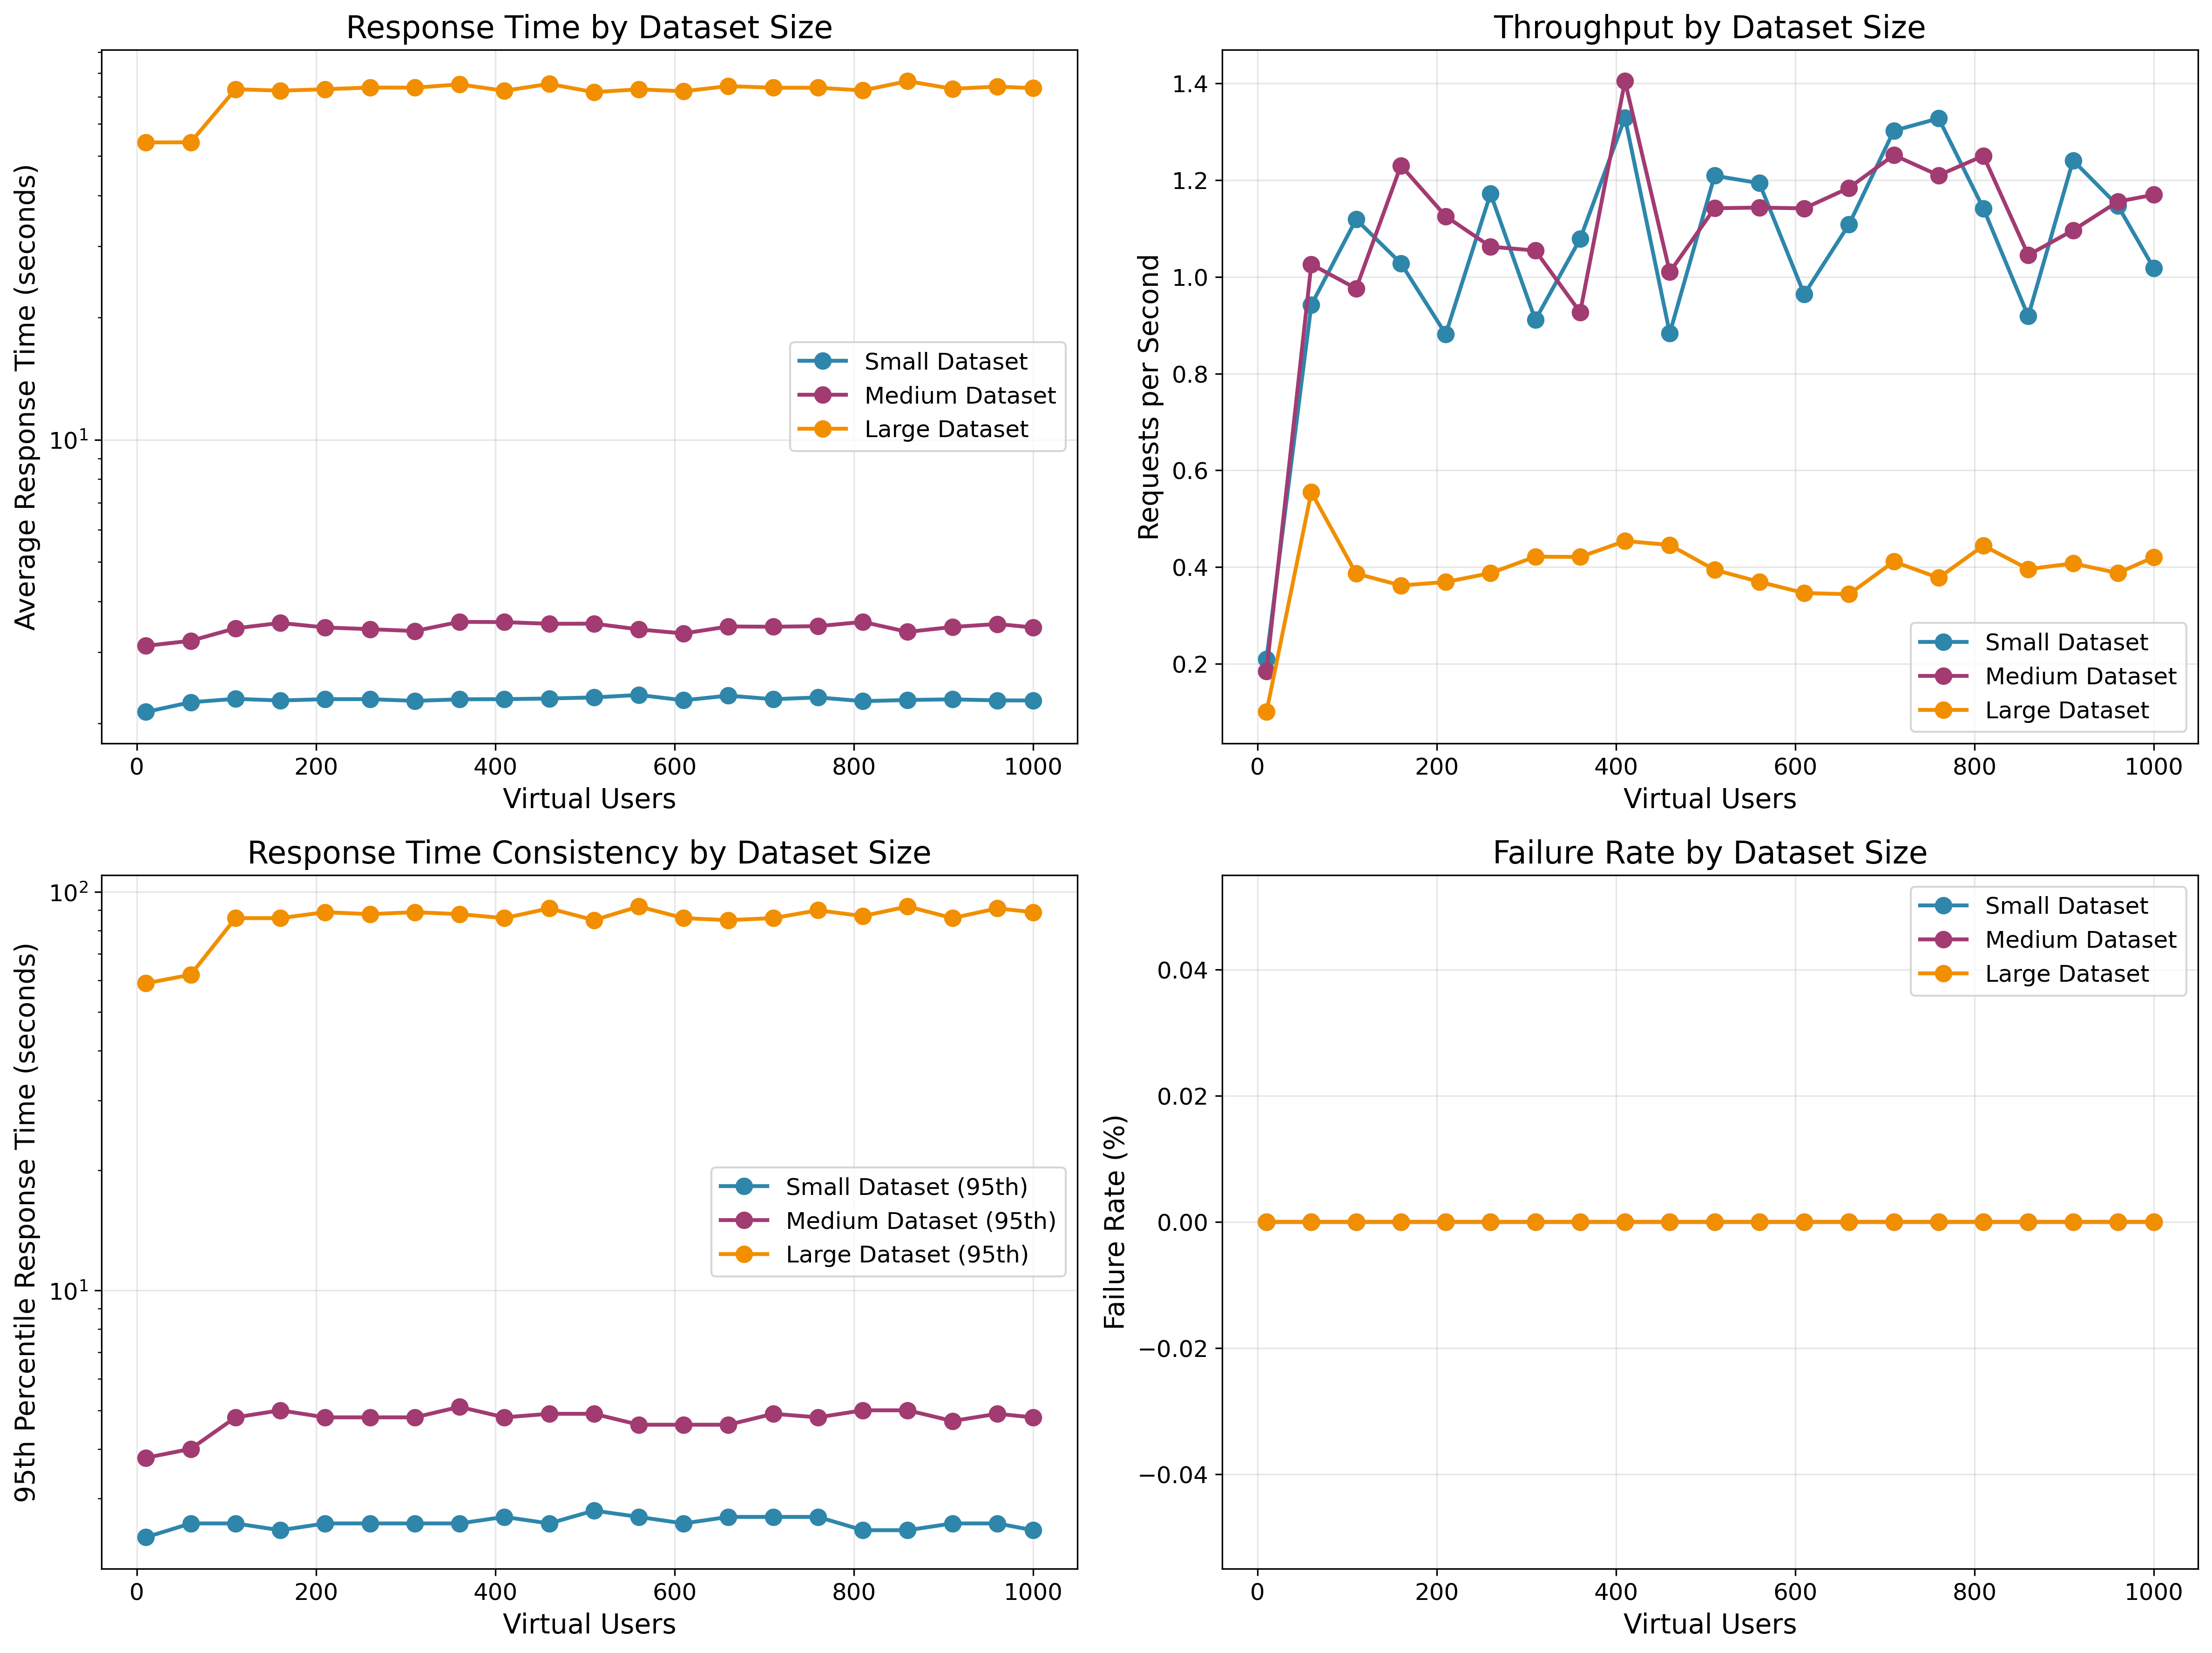
\includegraphics[width=\columnwidth]{loadtest_results/dataset_size_analysis.png}
\caption{Detailed comparison of average response times, throughput, 95th percentile response times, and failure rates across Small, Medium, and Large dataset sizes under varying virtual user loads.}
\label{fig:dataset_analysis}
\end{figure}

\textbf{Response Time Performance:} As depicted in Figure~\ref{fig:dataset_analysis} (top-left panel), average response times varied significantly with dataset size. The \textit{Small Dataset} consistently yielded the fastest response times, remaining below 5 seconds even at 1000 VUs (e.g., 2.28s at 1000 VUs, as shown in Table~\ref{tab:load_test_summary_detailed}). The \textit{Medium Dataset} showed a moderate increase, with average response times typically between 20-30 seconds (e.g., 3.5s at 1000 VUs). The \textit{Large Dataset} presented the highest response times, averaging around 70-80 seconds (e.g., 73.5s at 1000 VUs). This direct correlation is further exemplified in Table~\ref{tab:load_test_summary_detailed}, which summarizes performance at low and high user loads. At 1000 VUs, the average response time for the Large dataset (73.47 s) is drastically higher than for the Medium (3.47 s) and Small (2.28 s) datasets, clearly demonstrating the performance impact of data size. The 95th percentile response times (Figure~\ref{fig:dataset_analysis}, bottom-left panel, and Figure~\ref{fig:dataset_heatmaps}, bottom-left panel) also show a similar trend, indicating that the impact of dataset size affects the vast majority of user experiences.

\begin{figure}[htbp]
\centering
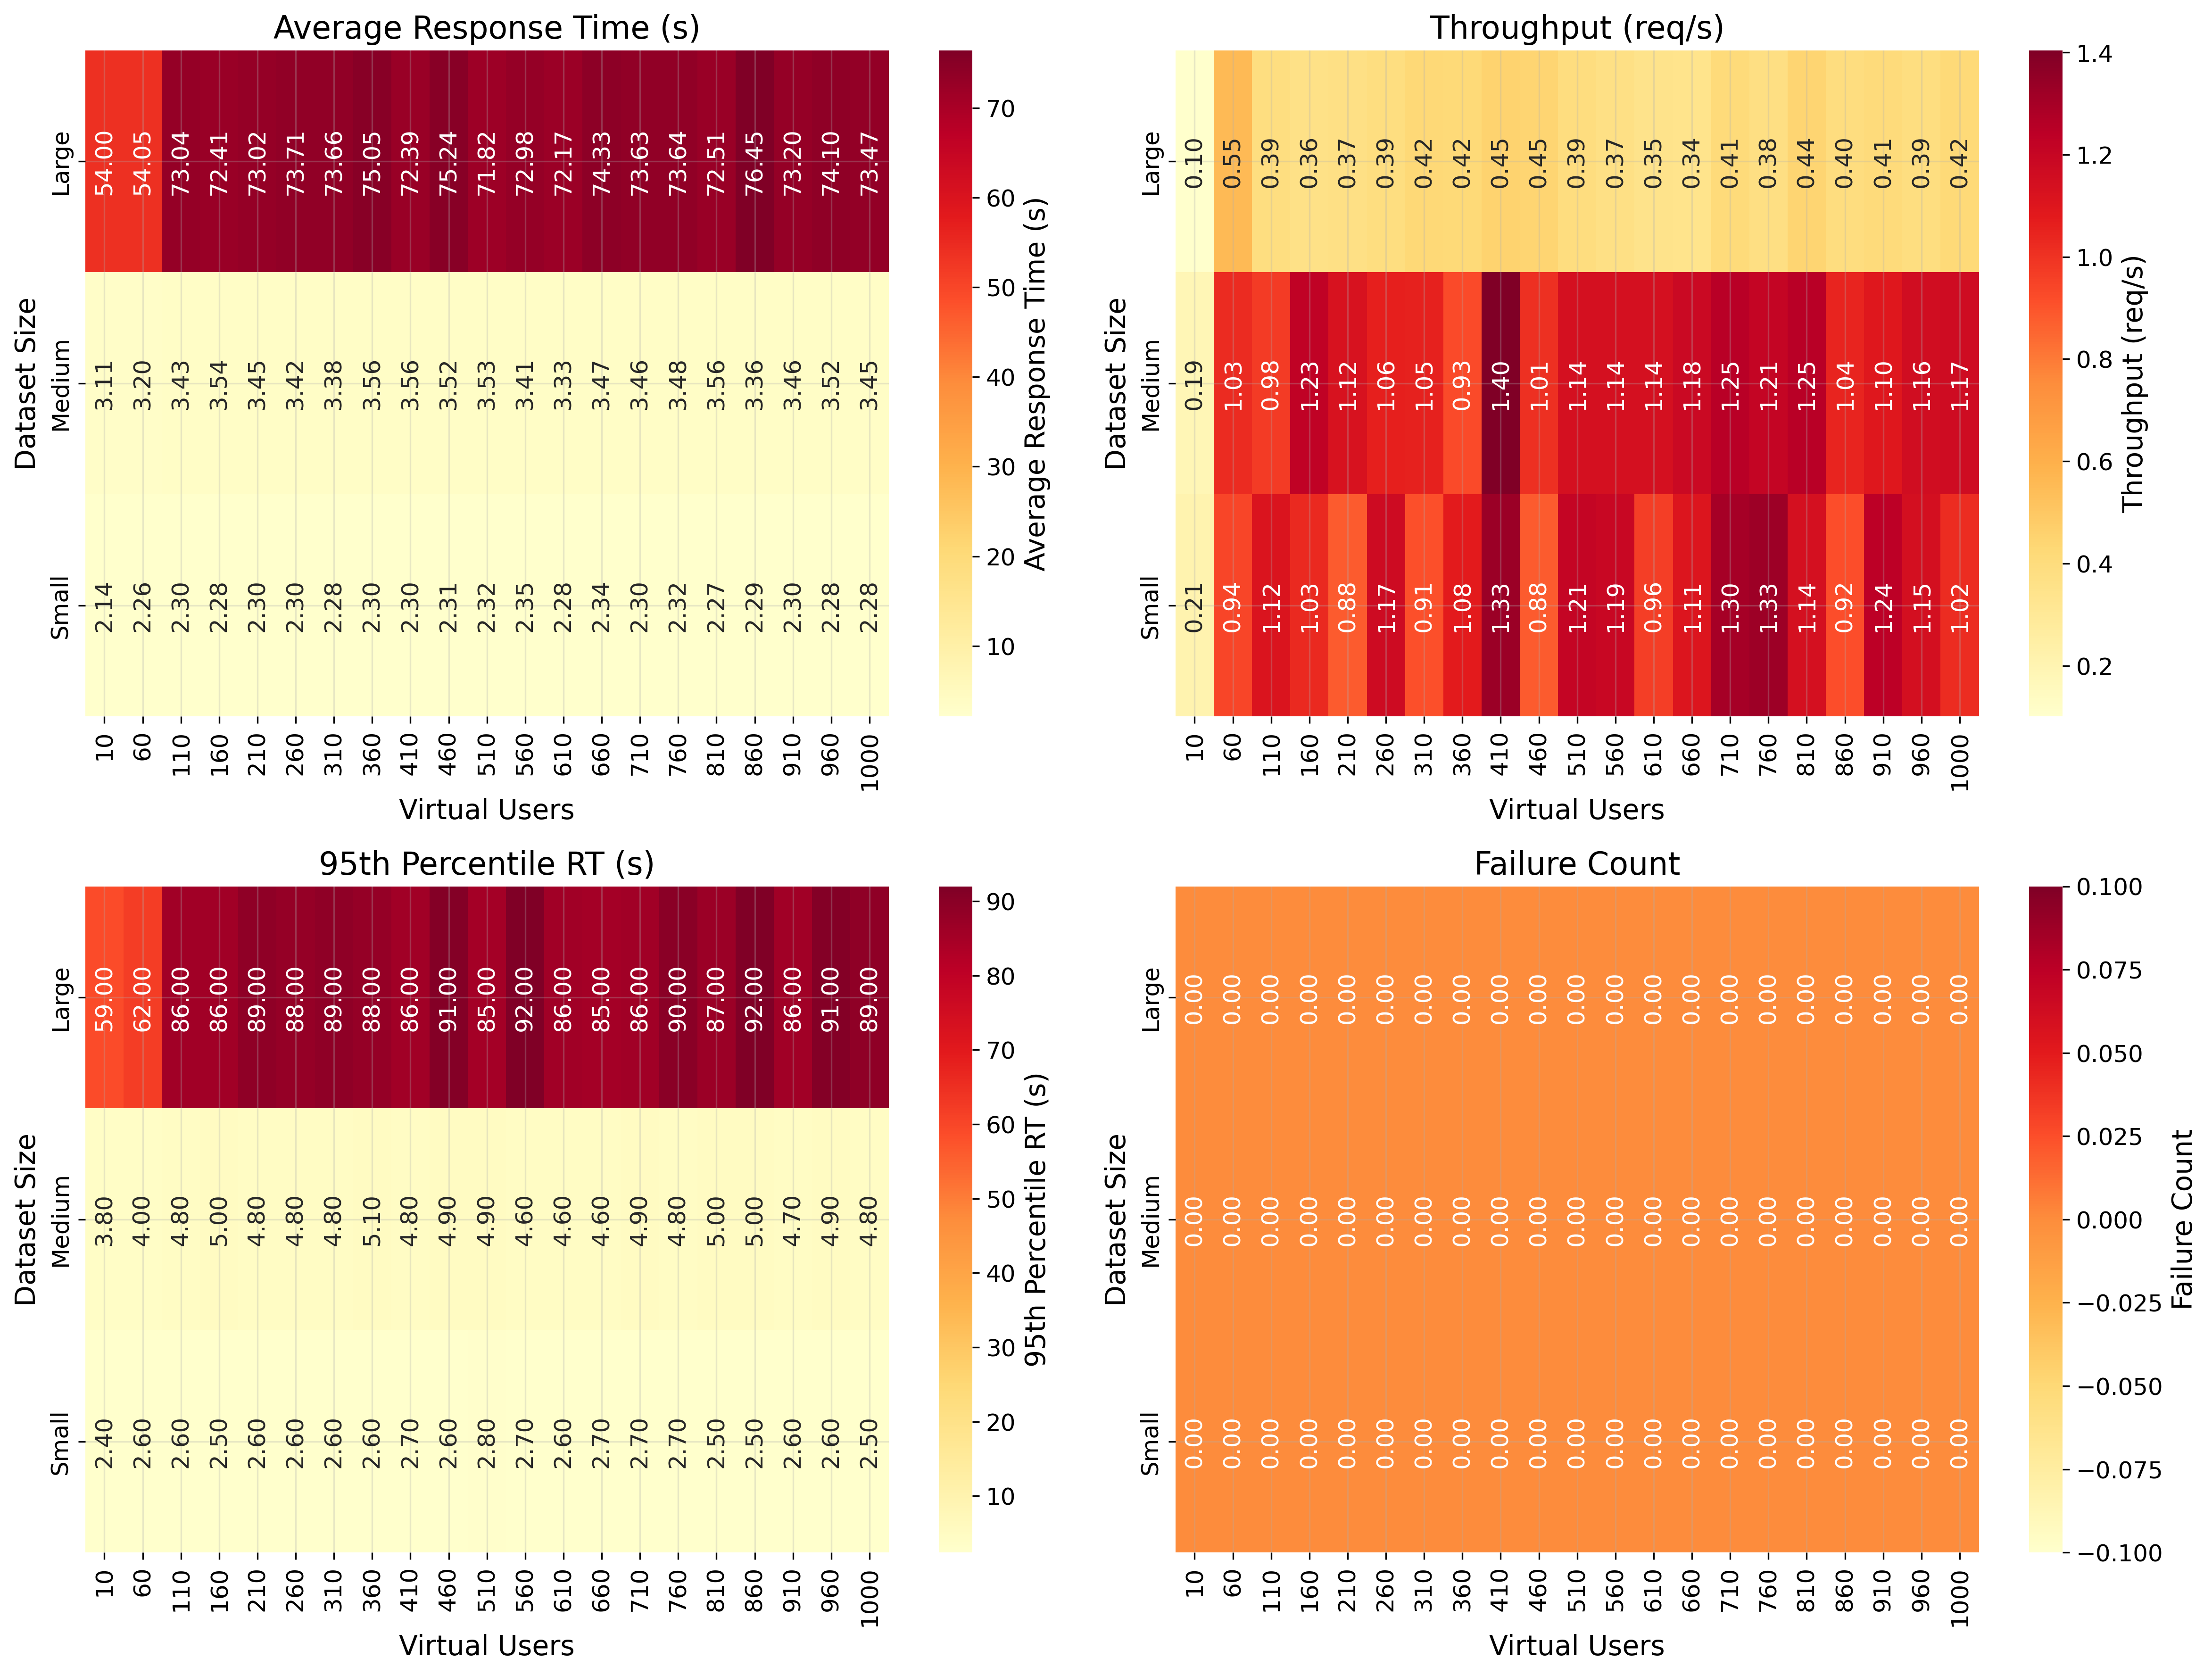
\includegraphics[width=\columnwidth]{loadtest_results/dataset_size_heatmaps.png}
\caption{Heatmap visualizations illustrating the distribution of average response times, throughput, 95th percentile response times, and failure counts across different dataset sizes and virtual user loads.}
\label{fig:dataset_heatmaps}
\end{figure}

\textbf{Throughput Capacity:} Figure~\ref{fig:dataset_analysis} (top-right panel) illustrates the throughput performance. The \textit{Small Dataset} and \textit{Medium Dataset} achieved similar peak throughput values, ranging from 0.8 to 1.4 requests/second, and demonstrated robust scaling behavior as user loads increased. In contrast, the \textit{Large Dataset} exhibited significantly lower throughput, stabilizing around 0.4-0.5 requests/second. This suggests that while BioMark can process larger files, the per-second processing capacity is substantially reduced due to the increased computational overhead associated with larger data volumes.

\begin{table}[htbp]
\centering
\caption{Summary of Load Test Performance Metrics at Low, Medium, and High Virtual User (VU) Loads for Each Dataset Size.}
\label{tab:load_test_summary_detailed}
\small
% Adjust spacing between columns
\setlength{\tabcolsep}{4pt} 

% Column definitions:
% 'll' for the first two text columns (left aligned)
% 'wc{1.7cm}' for the other three columns (centered with specified, narrower width)
\begin{tabular}{llwc{1.7cm}wc{1.7cm}wc{1.7cm}}
\toprule
\textbf{\thead{Dataset \\ Size}} & \textbf{\thead{Virtual \\ Users}} & \thead{Avg. Response \\ Time (s)} & \thead{95th Percentile \\ RT (s)} & \thead{Throughput \\ (req/s)} \\
\midrule
\multirow{3}{*}{\textbf{Small}}  & 60  & 2.26  & 2.6  & 0.94 \\
 & 510 & 2.30  & 2.6  & 1.14 \\
 & 1000& 2.28  & 2.5  & 1.17 \\
\addlinespace % Adds space between groups
\multirow{3}{*}{\textbf{Medium}} & 60  & 3.20  & 4.0  & 1.02 \\
 & 510 & 3.53  & 4.9  & 1.14 \\
 & 1000& 3.47  & 4.8  & 1.17 \\
\addlinespace % Adds space between groups
\multirow{3}{*}{\textbf{Large}}  & 60  & 54.05 & 59.0 & 0.55 \\
 & 510 & 71.82 & 85.0 & 0.39 \\
 & 1000& 73.47 & 91.0 & 0.38 \\
\bottomrule
\end{tabular}
\end{table}

The load test results underscore that BioMark effectively handles varying data sizes, maintaining 0\% failure rates across all tested conditions. However, performance metrics like response time and throughput are heavily influenced by the size of the uploaded dataset. Small and medium datasets are processed efficiently, making BioMark highly responsive for typical biomarker panels. For large, high-dimensional omics datasets, while the system remains reliable, processing times naturally increase, indicating a need for careful consideration of computational resources and potential optimizations for extremely large files in future developments. These findings provide crucial insights for capacity planning and user expectations when analyzing diverse omics data with BioMark.
\subsection{Analysis Time Evaluation}
This subsection details the execution times for various computationally intensive analytical tasks performed by BioMark, highlighting the tool's efficiency in processing complex biomarker data. The analysis times were recorded on the same server environment used for load testing.

Analysis time was evaluated for critical operations such as differential analysis, clustering, and classification across two distinct datasets: the prostate cancer dataset (137 samples, 27,828 features) and the breast cancer dataset (108 samples, 16,382 features). The detailed execution times for each analysis type are presented in Table~\ref{tab:analysis_times}.

% Using 'table' for single-column width
\begin{table}[htbp]
\centering
 \caption{Analysis Execution Times for Prostate and Breast Cancer Datasets}
\label{tab:analysis_times} 
\small
% Using 'tabularx' to ensure content fits within column width
% X: auto-wrapping text column, r: right-aligned number/time column
\begin{tabularx}{\columnwidth}{X r r}
\toprule
% Shortened column headers
\textbf{Analysis Type} & \textbf{Prostate} & \textbf{Breast} \\
\midrule
\multicolumn{3}{l}{\textit{Differential Analysis}} \\
SHAP & 33 s & 18 s \\
LIME & 73 s & 42 s \\
ANOVA & 7 s & 7 s \\
T-test & 20 s & 15 s \\
XGBoost Feat. Imp. & 9h 23m 07s & 2h 57m \\
RF Feat. Imp. & 8m 30s & 4m 58s \\
Permutation Feat. Imp. & 2h 28m 18s & 51m 47s \\
\midrule
\multicolumn{3}{l}{\textit{Clustering Analysis}} \\
PCA & 10 s & 10 s \\
t-SNE & 12 s & 11 s \\
UMAP & 13 s & 11 s \\
\midrule
\multicolumn{3}{l}{\textit{Classification Analysis}} \\
Logistic Regression & 11 s & 9 s \\
Random Forest & 12 s & 11 s \\
XGBClassifier & 38 s & 27 s \\
Decision Tree & 11 s & 9 s \\
Gradient Boosting & 3m 16s & 1m 29s \\
CatBoost Classifier & 1h 19m & 23m \\
AdaBoost Classifier & 55 s & 29 s \\
MLPClassifier & 17 s & 15 s \\
SVC & 11 s & 10 s \\
\bottomrule
\end{tabularx}
\end{table}
Table~\ref{tab:analysis_times} demonstrates that BioMark efficiently processes large and complex omics data within practical timeframes for many critical operations. For instance, most clustering and simpler classification models (e.g., PCA, Logistic Regression, Decision Tree, SVC) complete within seconds, providing rapid insights. Differential analysis methods like ANOVA and T-test also execute quickly.

However, certain computationally intensive machine learning methods, particularly in differential analysis (e.g., XGBoost Feature Importance, Permutation Feature Importance) and classification (e.g., CatBoosting Classifier), require significantly extended durations. For the prostate cancer dataset, XGBoost Feature Importance took approximately 9.4 hours (\SI{33787}{\second}), and Permutation Feature Importance took around 2.5 hours (\SI{8898}{\second}). Similarly, CatBoosting Classifier required about 1.3 hours (\SI{4741}{\second}). While these durations are substantial, they are typical for high-dimensional feature importance calculations and complex model training on large datasets. The breast cancer dataset, being smaller, generally resulted in faster execution times for these computationally demanding tasks (e.g., XGBoost Feature Importance: \SI{10620}{\second} $\approx$ 2.9 hours; CatBoosting Classifier: \SI{1381}{\second} $\approx$ 23 minutes).

These measurements highlight BioMark's capability as a versatile tool for biomarker discovery and validation. While common analytical tasks are highly responsive, users should anticipate longer processing times for advanced, computationally intensive algorithms on high-dimensional omics data, especially for larger datasets.

\subsection{Case Study on Prostate Cancer}
This section details the application of the BioMark web tool to a prostate cancer transcriptomics dataset (137 samples, 27,828 gene transcripts, where 'Factors' column includes cancer/healthy status).

\subsubsection{Analysis Results}
\paragraph{Differential Analysis and Biomarker Identification}
Differential analysis was conducted to identify statistically significant biomarkers capable of distinguishing between prostate cancer and healthy samples, employing BioMark's comprehensive suite of analytical methods. This process leverages both traditional statistical approaches and advanced machine learning-based feature explanation techniques, providing a multi-faceted view of the molecular signatures driving the disease.

The analysis began with classical statistical tests like ANOVA to identify biomarkers with significant mean expression differences between the cancer and healthy cohorts. As shown in the ANOVA results (Fig.~\ref{fig:prostate_anova_features}), biomarkers such as \textit{LOC105374013}, \textit{DANCR}, and \textit{PCA3} demonstrated high F-values, indicating strong statistical power in differentiating the two groups based on their expression levels alone.

To gain deeper, model-driven insights, we utilized explainability methods like SHAP (SHapley Additive exPlanations) and LIME (Local Interpretable Model-agnostic Explanations). Unlike ANOVA, which assesses each feature in isolation, these methods evaluate a biomarker's contribution within the context of a predictive model that learns complex interactions. The SHAP Summary Plot (Fig.~\ref{fig:prostate_shap_summary}) offers a global perspective on feature importance. For instance, it reveals that high expression of biomarkers like \textit{NEK5} and \textit{LOC105374013} (indicated by red dots) consistently yields high positive SHAP values, pushing the model's prediction towards cancer. Conversely, low expression of these same markers (blue dots) contributes to a "healthy" prediction. This visualization powerfully illustrates not only the importance of each biomarker but also the direction and magnitude of its effect across all samples.

This global view is complemented by instance-level explanations. The SHAP Heatmap (Fig.~\ref{fig:prostate_heatmap}) visualizes the collective behavior of SHAP values across the entire dataset, clearly delineating the cancer and healthy cohorts through distinct biomarker contribution patterns. For a more granular view, SHAP Waterfall plots (Fig.~\ref{fig:prostate_shap_waterfall_new}) deconstruct the prediction for individual samples. They illustrate precisely how each biomarker contributes to shifting the model's output from the baseline to the final prediction for both a representative cancer sample and a healthy one. For example, in the cancer sample, high expression of \textit{RUSC1} and \textit{NEK5} are shown as primary drivers of the cancer classification.

Similarly, the LIME plot (Fig.~\ref{fig:prostate_lime_bar}) provides a local explanation for a single cancer sample, highlighting that high expression of \textit{STAT6} and \textit{MCM8} were key contributors to its specific classification. The slight differences in top biomarkers between global methods (SHAP Summary, ANOVA) and local methods (LIME, SHAP Waterfall) underscore the biological heterogeneity within the cancer group and demonstrate BioMark's capacity to capture both population-level trends and patient-specific molecular events. This dual approach, combining robust statistical validation with nuanced model-based interpretation, facilitates a more comprehensive identification of clinically relevant biomarkers.

% FIGURE DEFINITIONS (Original file paths used)

\begin{figure}[htbp]
 \centering
 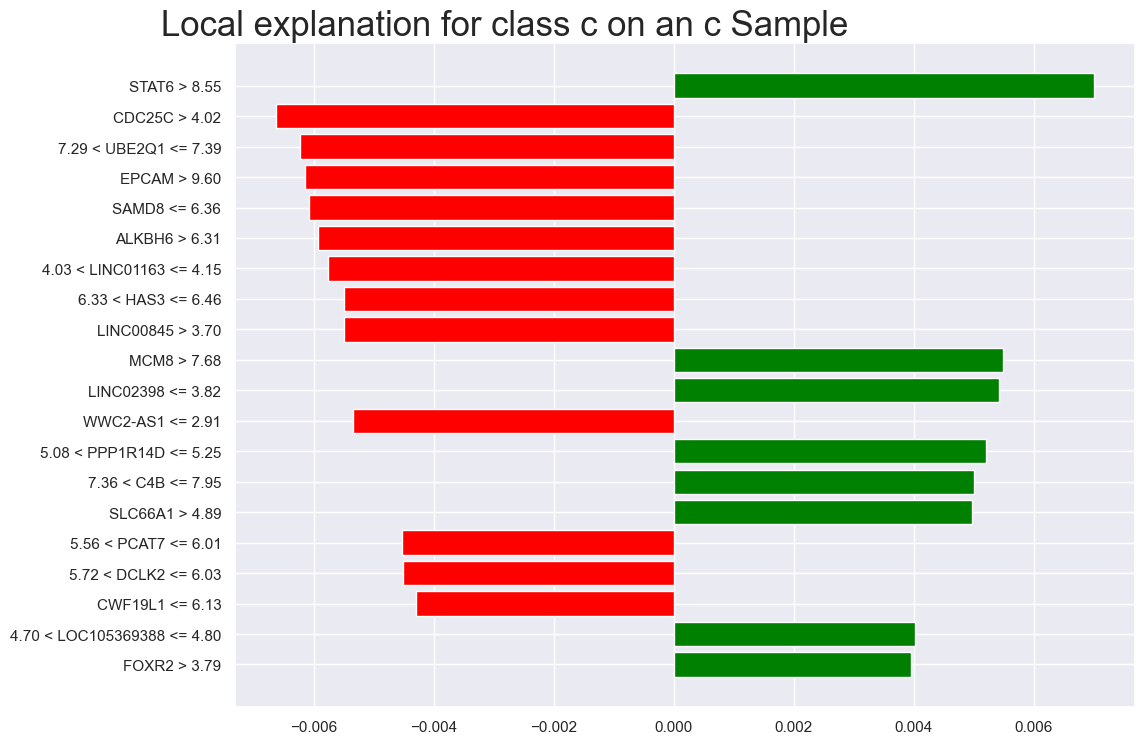
\includegraphics[width=1\linewidth]{prostate_cancer_figures/differential/lime_local_explanation_plot_c.png}
 \caption{LIME plot illustrating top contributing biomarkers for a single prostate cancer sample prediction.}
 \label{fig:prostate_lime_bar}
\end{figure}

\begin{figure}[htbp]
 \centering
 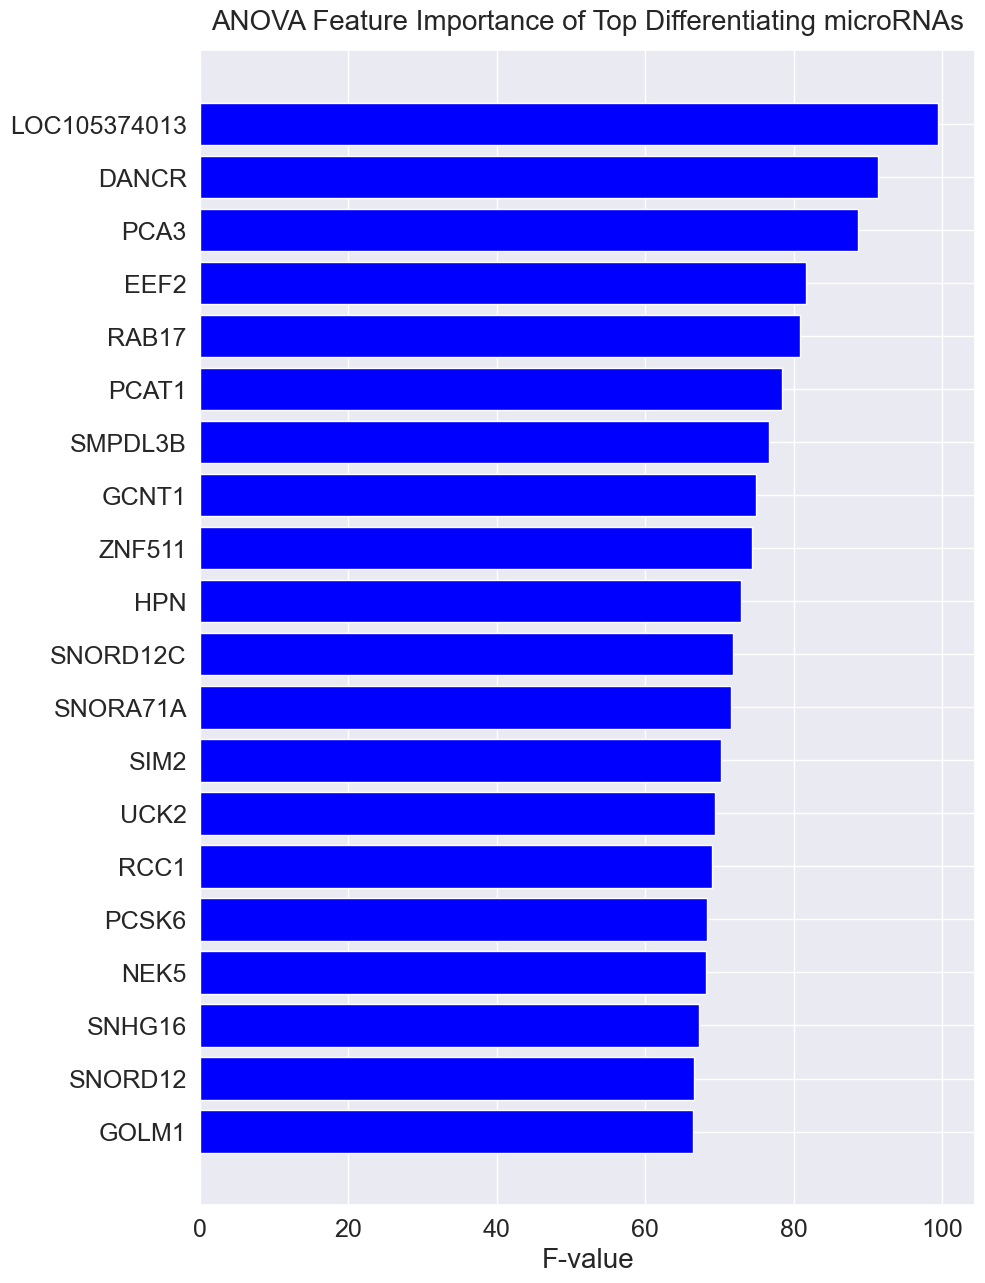
\includegraphics[width=0.9\linewidth]{prostate_cancer_figures/differential/anova_features_plot.png}
 \caption{The most discriminative biomarkers detected by ANOVA test in the prostate cancer dataset. The graph shows the most significant features ranked according to the statistical significance of the difference between cancer and healthy samples.}
 \label{fig:prostate_anova_features}
\end{figure}

\begin{figure}[htbp]
 \centering
 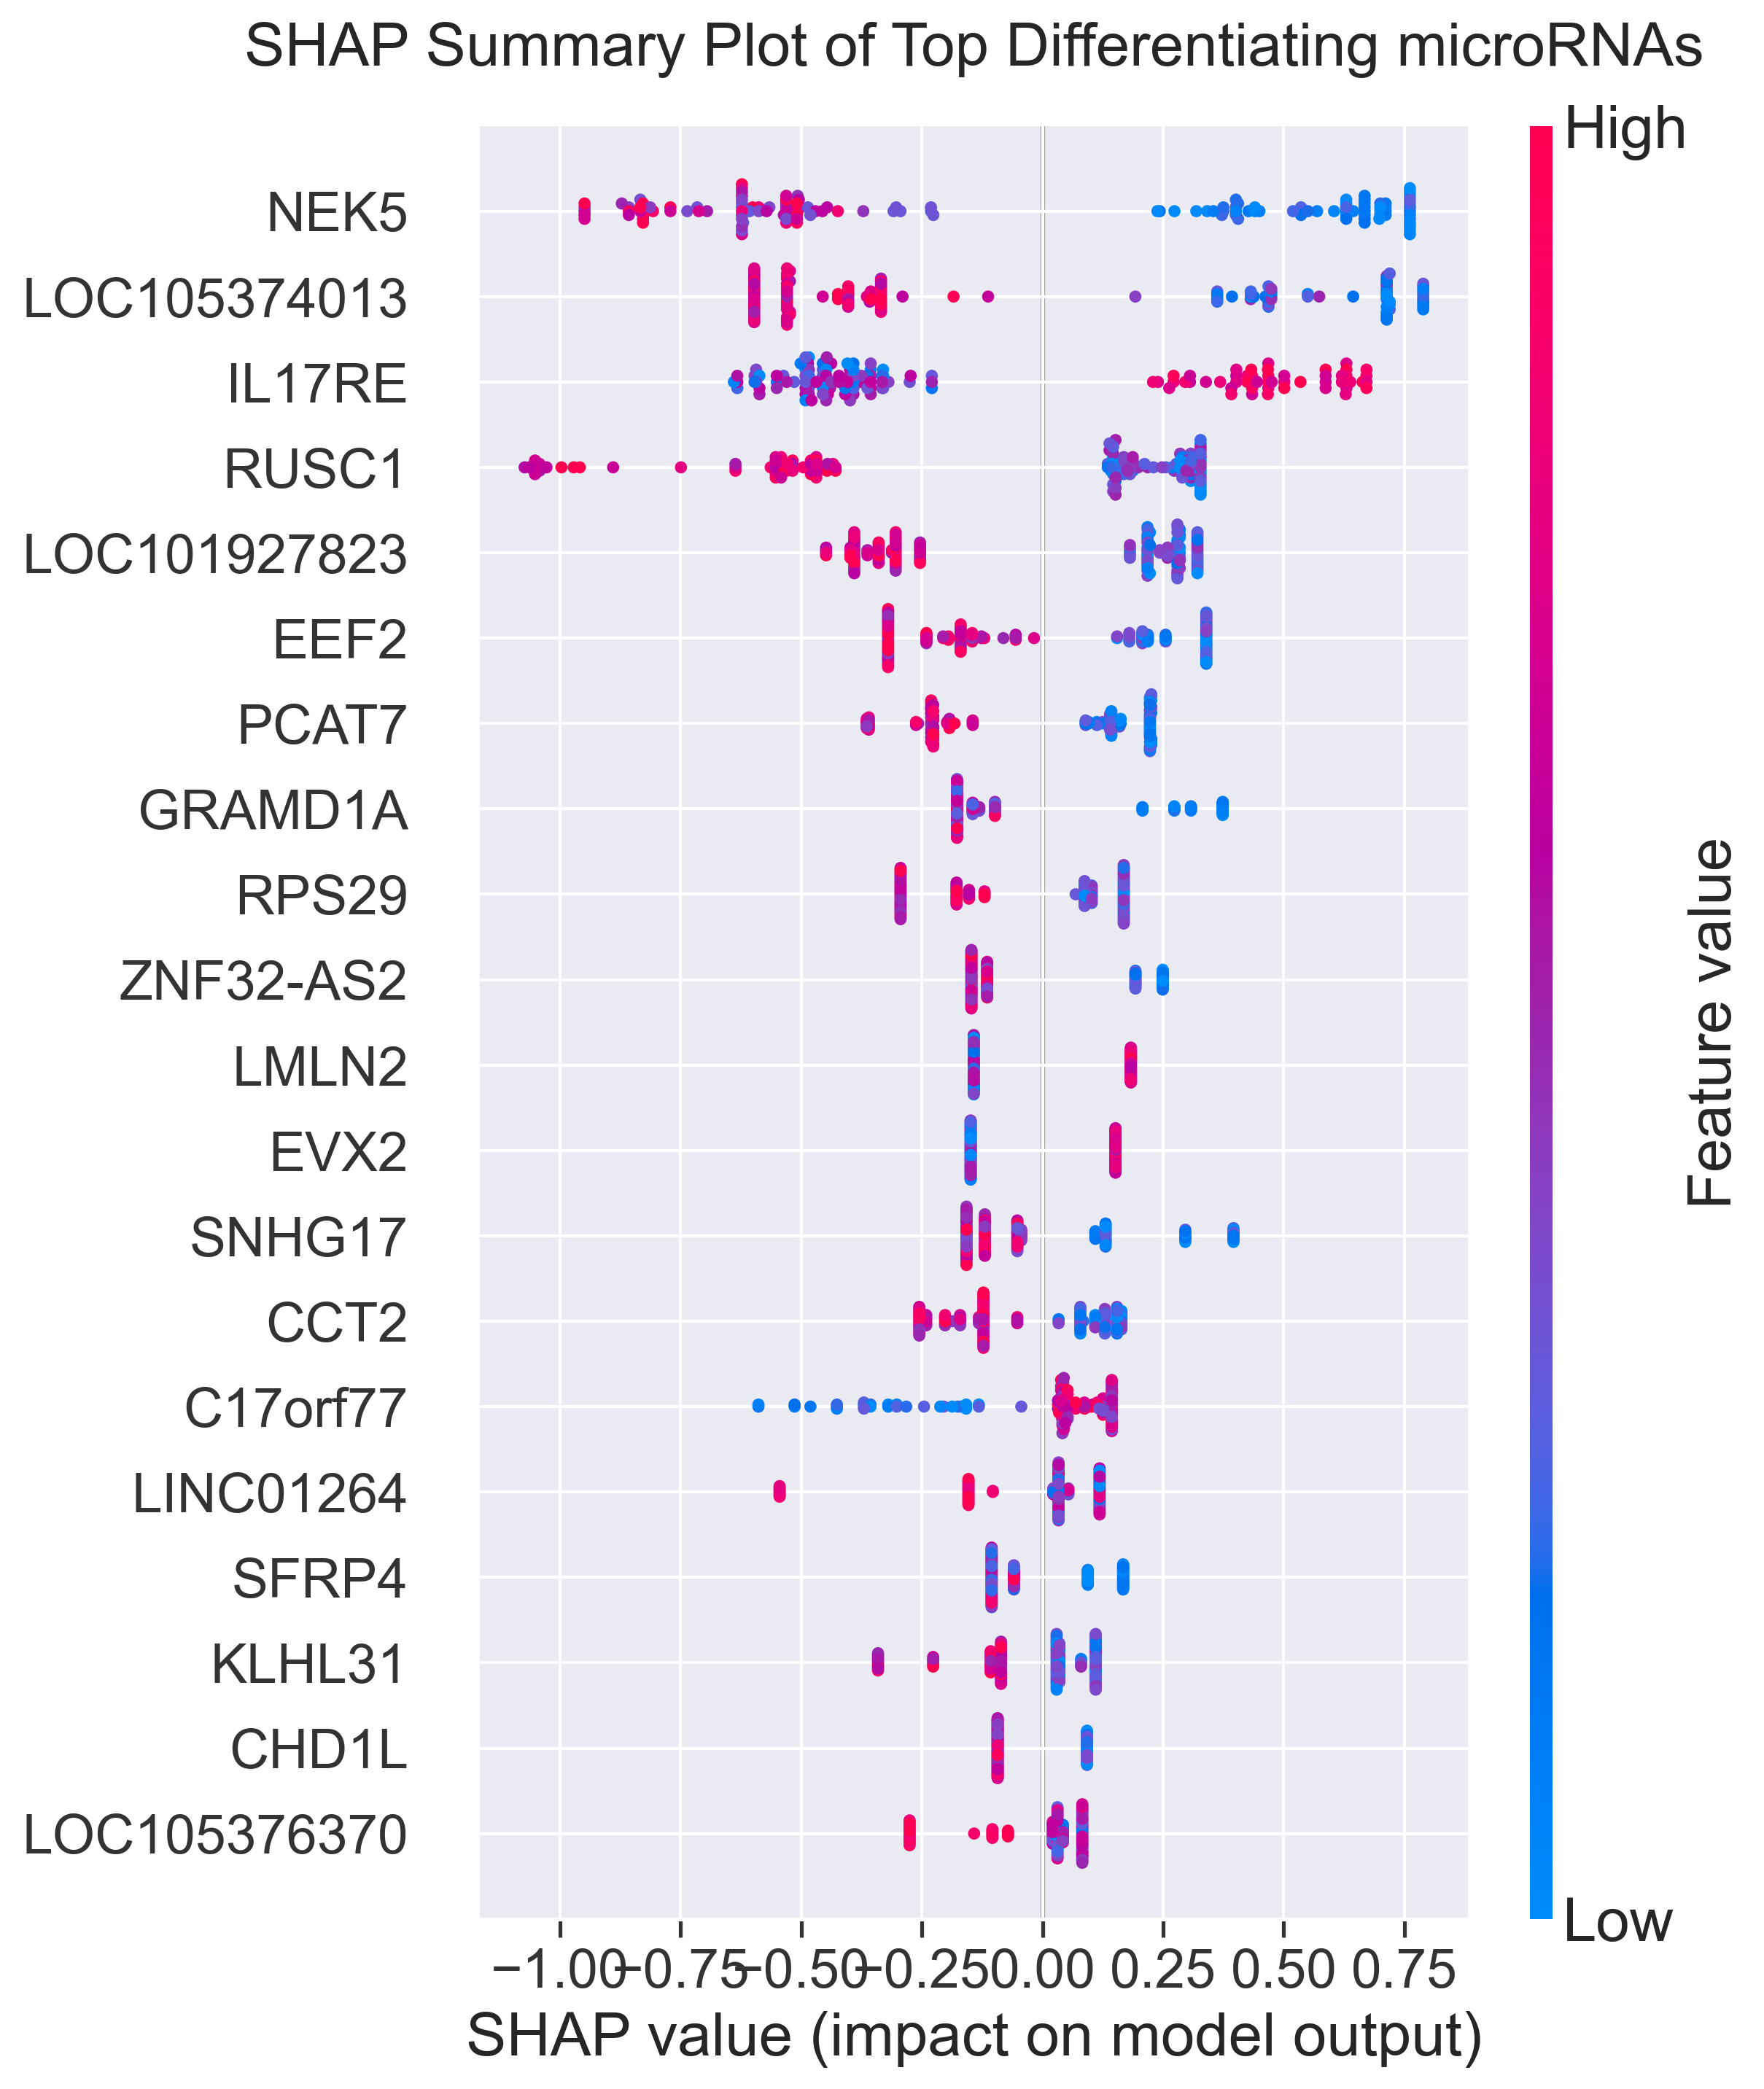
\includegraphics[width=0.9\linewidth]{prostate_cancer_figures/differential/shap_summary_plot_c_and_healthy.png}
 \caption{SHAP Summary Plot for Prostate Cancer Differential Analysis: Illustrating the overall impact and direction of influence for the most important biomarkers.}
 \label{fig:prostate_shap_summary}
\end{figure}

\begin{figure}[htbp]
 \centering
 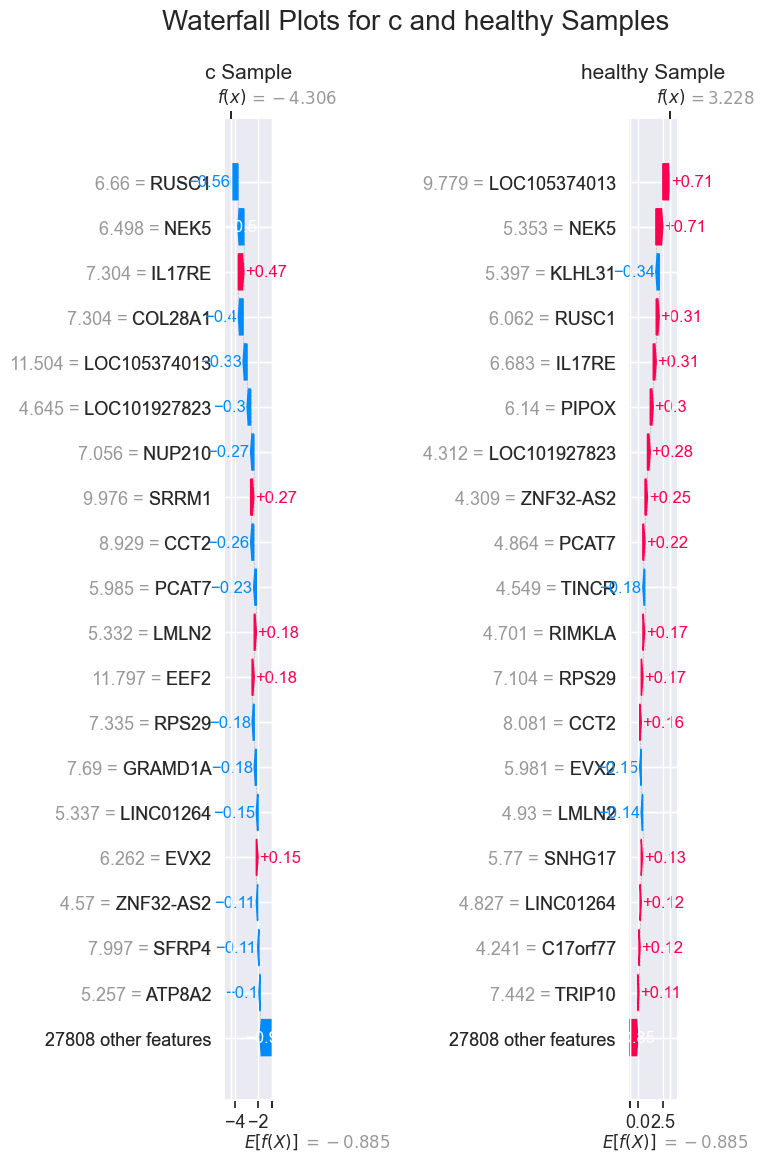
\includegraphics[width=0.8\linewidth]{prostate_cancer_figures/differential/shap_waterfall_subplots_c_and_healthy.png}
 \caption{SHAP Waterfall plots illustrating the model's prediction for a representative cancer sample and a healthy sample. The plots show how the contribution of each top biomarker pushes the prediction from the base value to the final output score.}
 \label{fig:prostate_shap_waterfall_new}
\end{figure}

\begin{figure}[htbp]
 \centering
 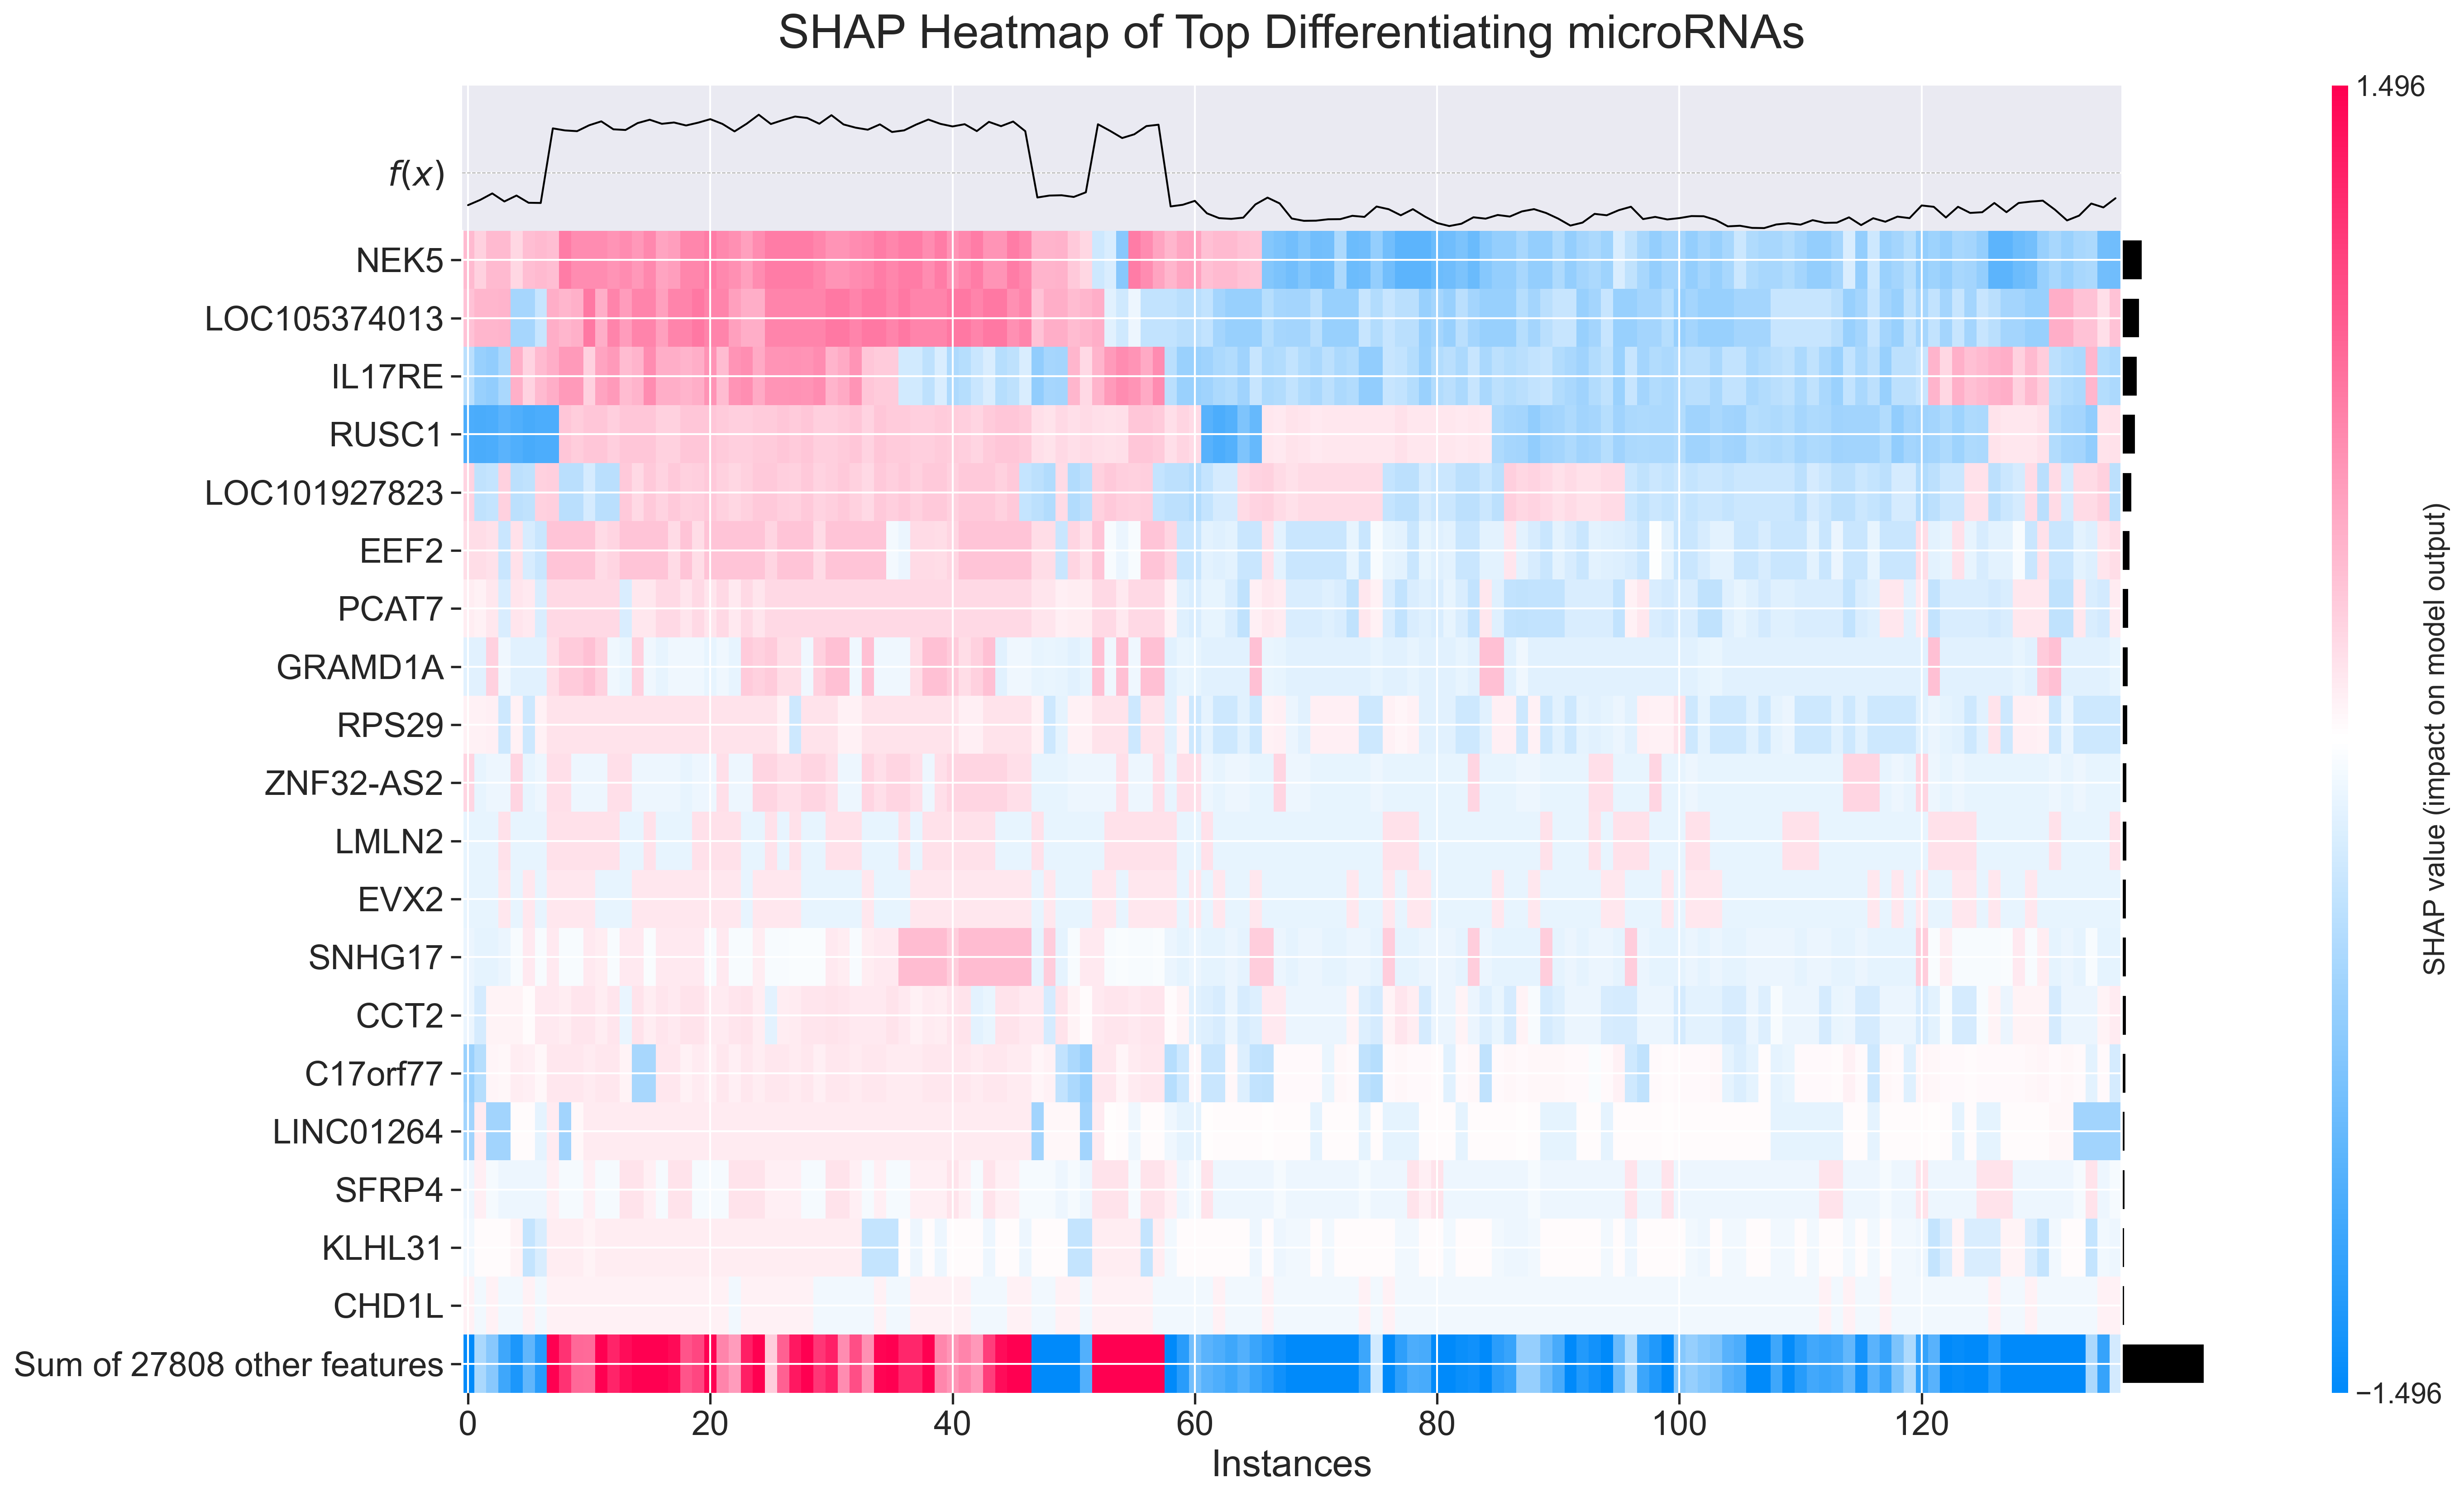
\includegraphics[width=1\linewidth]{prostate_cancer_figures/differential/shap_heatmap_plot_c_and_healthy.png}
 \caption{Heatmap of Top Differentiating Biomarkers in Prostate Cancer: Displaying expression patterns of top 19 biomarkers across cancer and healthy samples.}
 \label{fig:prostate_heatmap}
\end{figure}

\begin{figure}[htbp]
\centering
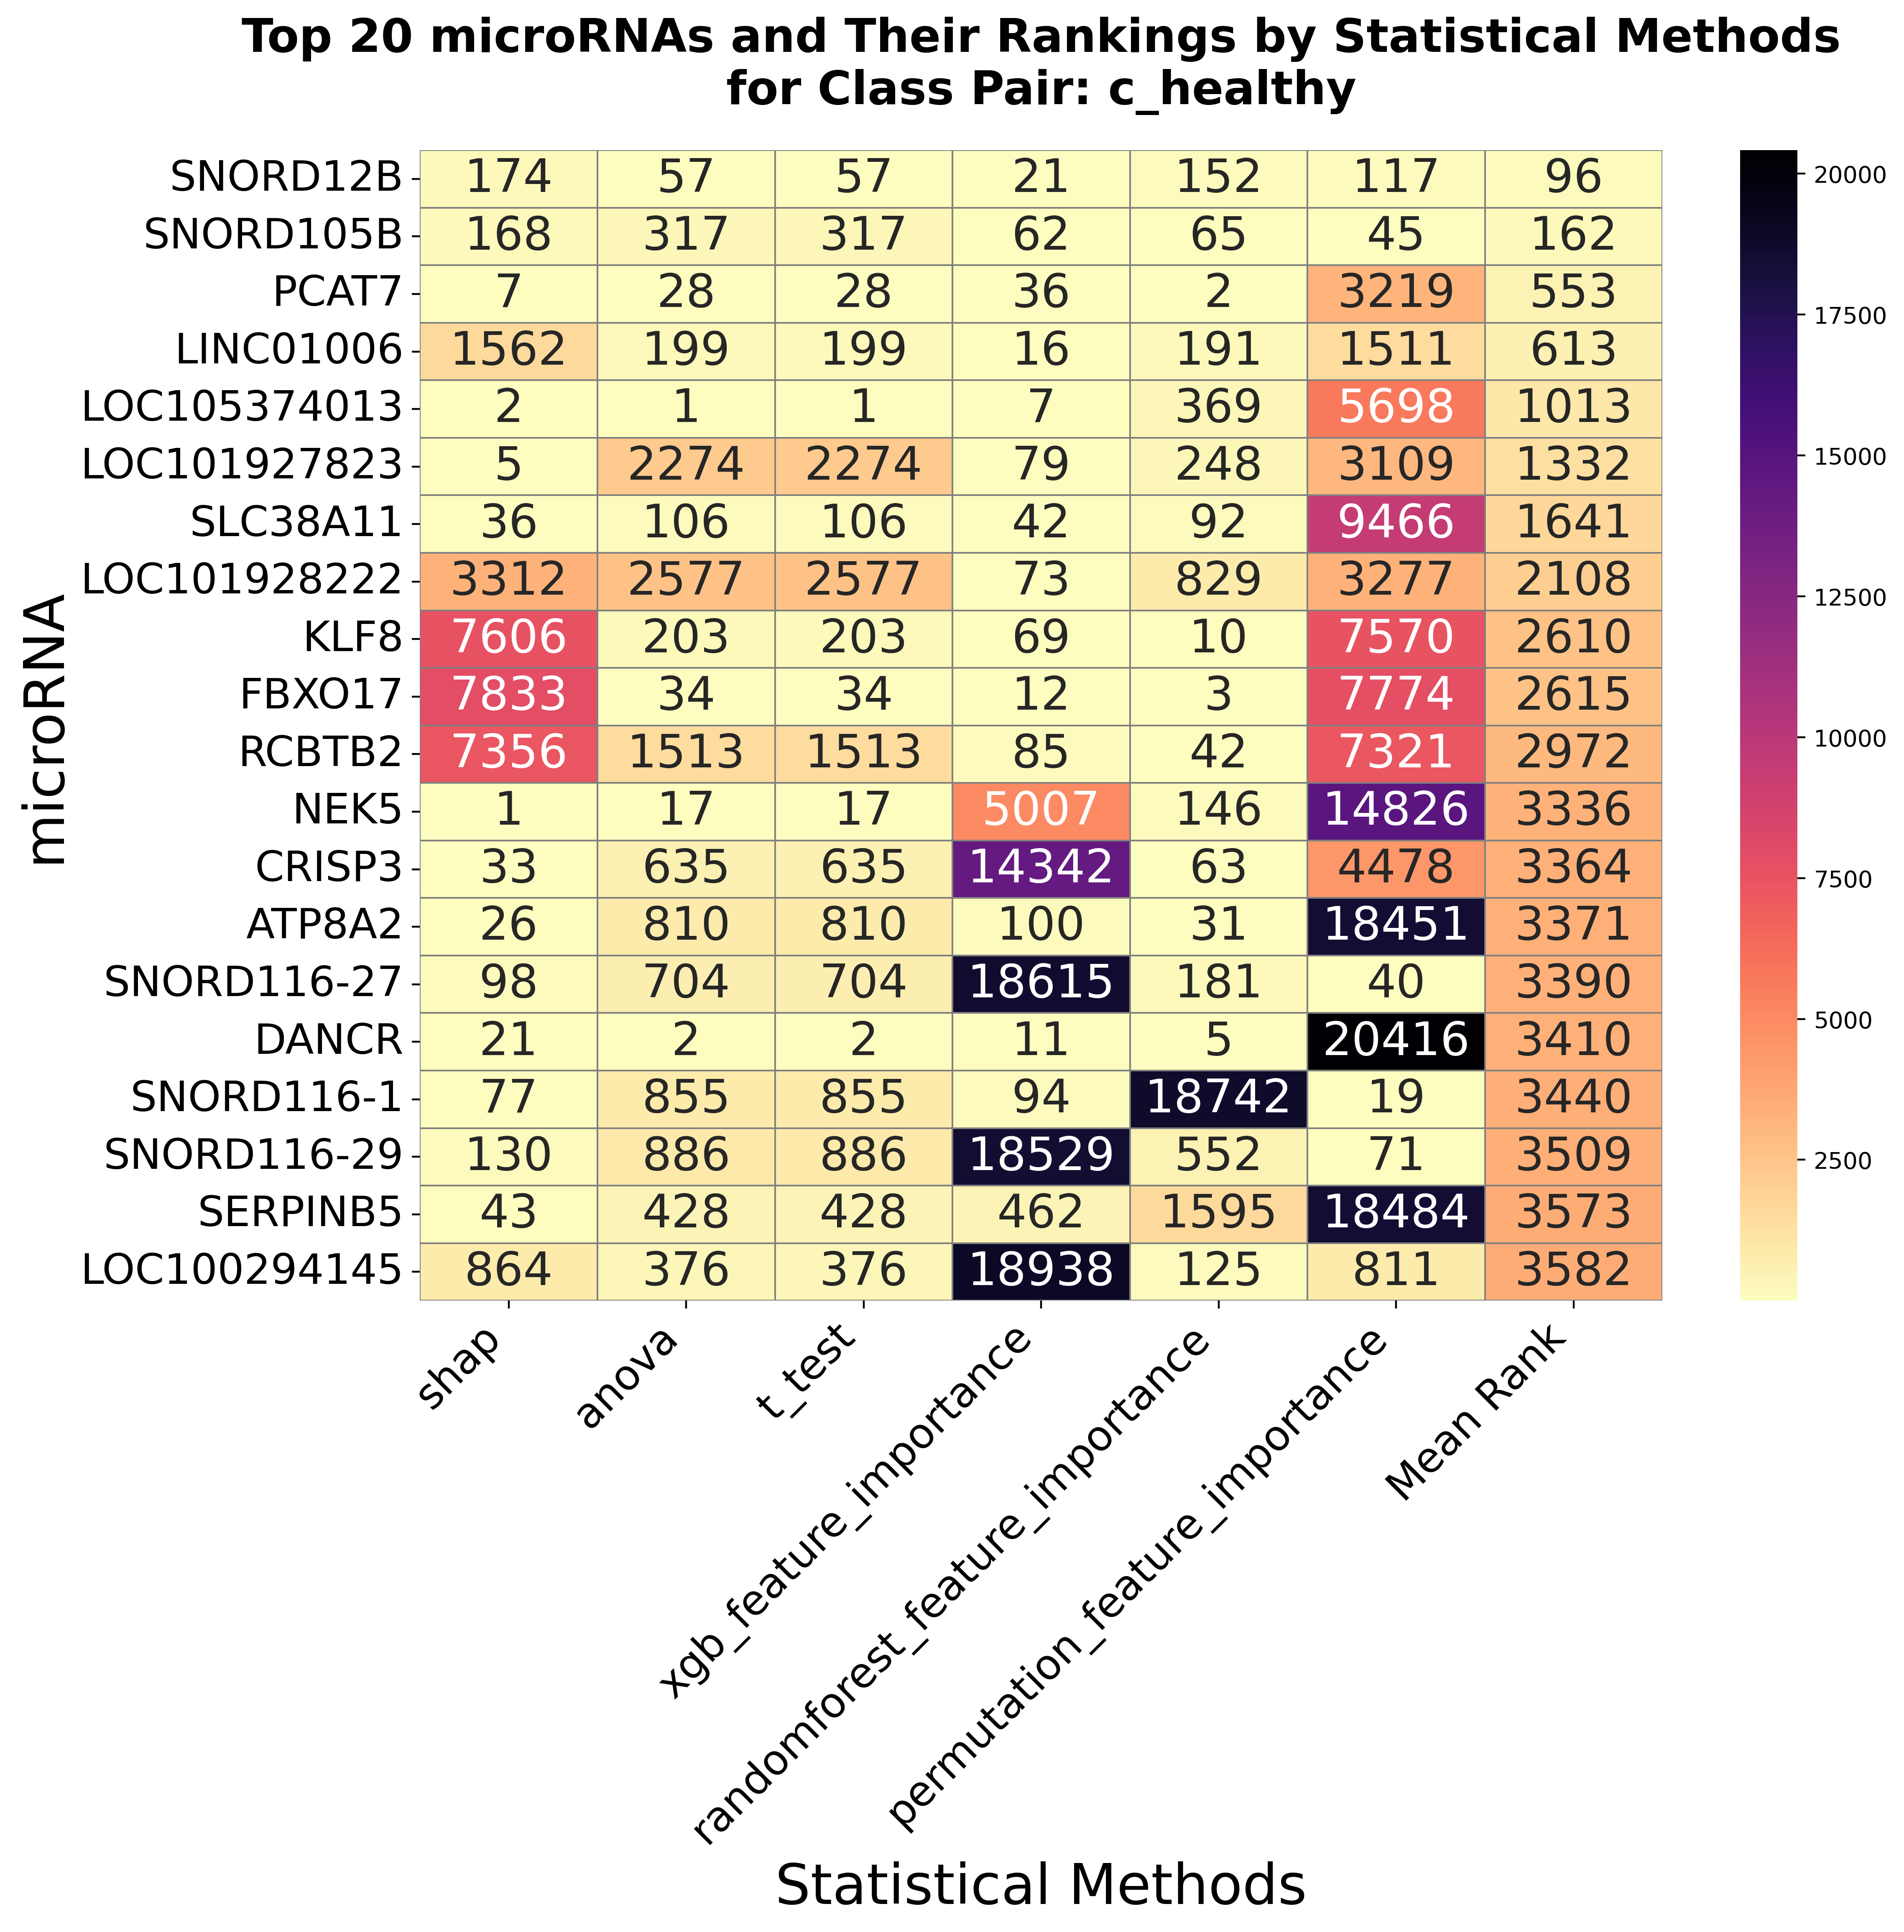
\includegraphics[width=1\linewidth]{prostate_cancer_figures/summary/summary_of_statistical_methods_plot.png}
\caption{Consolidated ranking of the top 20 differentiating biomarkers in Prostate Cancer. The plot summarizes feature importance scores from multiple methods (SHAP, LIME, ANOVA, etc.) to provide a robust consensus list of molecules distinguishing cancer samples from healthy controls.}
\label{fig:prostate_biomarker_summary}
\end{figure}

\subsubsection{Literature-Based Validation of Identified Biomarkers}
A key measure of BioMark's efficacy is its ability to identify biomarkers that are corroborated by existing scientific literature. Our analysis successfully pinpointed a range of molecules with well-documented roles in prostate cancer, thus validating our platform's analytical pipeline. For instance, top-ranked features identified by BioMark through its biomarker combination feature (Fig.~\ref{fig:prostate_biomarker_summary}) such as the lncRNAs \textbf{DANCR} and \textbf{PCAT7} are strongly supported by previous studies, which confirm their roles in promoting invasion and metastasis \cite{DANCR_prostate_2016, PCAT7_metastasis_2020}. Similarly, our tool highlighted \textbf{NEK5}, whose elevated expression is known to support tumor growth \cite{NEK5_prostate_2025}; \textbf{KLF8}, a co-activator for the androgen receptor linked to poor survival \cite{KLF8_prostate_2013}; \textbf{CRISP3}, a marker for a particularly aggressive molecular subtype of prostate cancer \cite{CRISP3_prostate_2014}; and the tumor suppressor \textbf{SERPINB5} (Maspin), whose loss is associated with cancer progression \cite{SERPINB5_prostate_2010}. Alongside these established markers, BioMark also prioritized candidates like \textit{SNORD12B} and \textit{SNORD105B}, for which direct links to prostate cancer are not yet extensively documented. This demonstrates BioMark's dual capability: robustly confirming known, clinically relevant biomarkers while simultaneously generating novel hypotheses for future experimental investigation.

\paragraph{Clustering Analysis}
Clustering analysis was performed to investigate the inherent structure of the prostate cancer dataset and to explore natural groupings among samples based on their biomarker profiles. This unsupervised approach utilizes dimensionality reduction techniques to visualize high-dimensional data in a lower-dimensional space, revealing patterns without prior knowledge of the sample labels (cancer or healthy). The analyses were conducted "After Feature Selection," meaning they were applied to a refined subset of the most informative biomarkers. This crucial preliminary step, as detailed in Section \ref{sec:feature_selection_mechanism_label}, reduces data noise and computational complexity, allowing the algorithms to focus on the strongest biological signals and thus produce clearer, more meaningful visualizations.

To achieve this, we employed three powerful dimensionality reduction methods: Principal Component Analysis (PCA), t-Distributed Stochastic Neighbor Embedding (t-SNE), and Uniform Manifold Approximation and Projection (UMAP), all offered in Biomark. The results, visualized in 3D space, consistently demonstrate a striking separation between the cancer and healthy samples.

As a linear method, PCA identifies the axes of maximum variance in the data. The resulting PCA plot (Fig.~\ref{fig:prostate_pca}) shows a clear and effective separation, with the healthy samples forming a tight, distinct cluster and the cancer samples forming another, more dispersed group. This indicates that a significant linear component of the variation in the biomarker data is sufficient to distinguish the two groups.

To capture more complex, non-linear relationships, we applied t-SNE and UMAP. The t-SNE method, which excels at preserving local neighborhood structures, also revealed a very strong separation between the two classes (Fig.~\ref{fig:prostate_tsne}), further confirming that the groups are distinct even when considering non-linear patterns. Similarly, UMAP, which effectively balances the preservation of both local and global data structure, provided the most striking visualization (Fig.~\ref{fig:prostate_umap}). It produced exceptionally compact and well-defined clusters with a pronounced margin between them, reinforcing the robustness of the identified biomarker signature.

The convergence of these three distinct methods—linear (PCA) and non-linear (t-SNE, UMAP)—on the same conclusion provides powerful evidence for the validity of the selected biomarkers. The ability of these unsupervised techniques to so clearly partition the samples based on their biological status underscores the fundamental transcriptomic differences between cancerous and healthy prostate tissue.


% FIGURE DEFINITIONS (Prostate Cancer Clustering)

\begin{figure}[htbp]
 \centering
 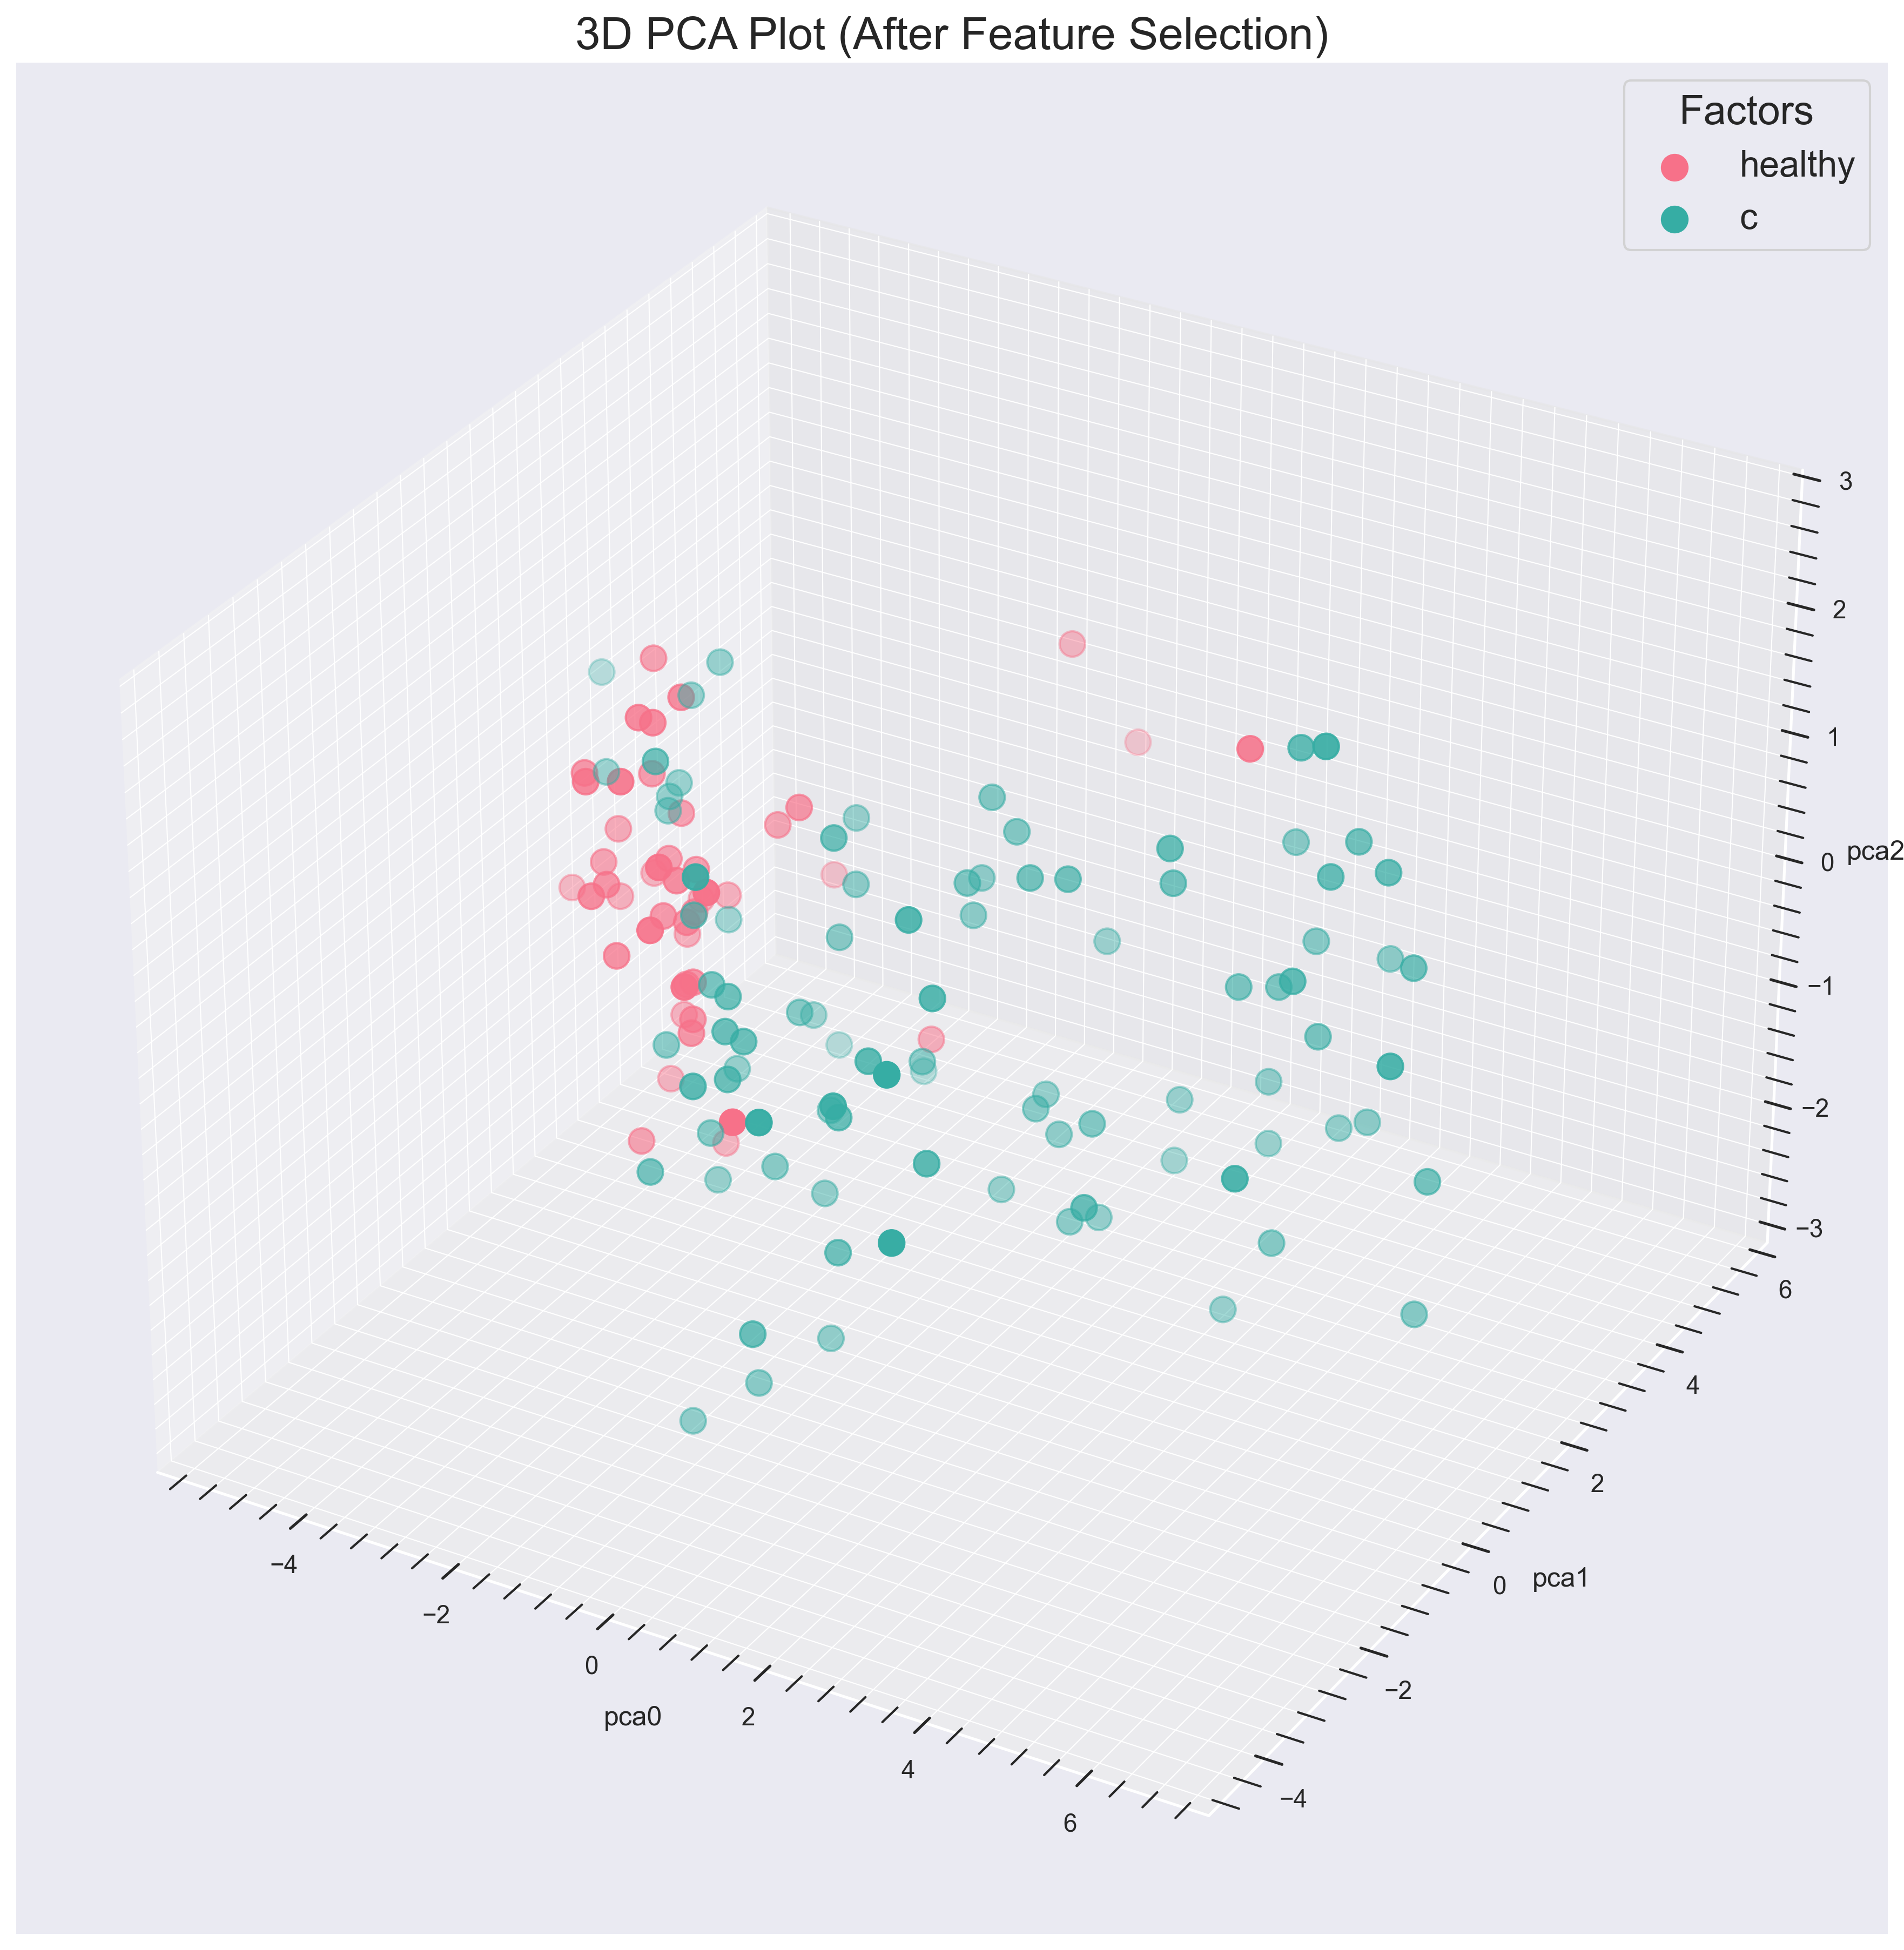
\includegraphics[width=\linewidth]{prostate_cancer_figures/clustering/after_feature_selection/3D_pca_plot.png}
 \caption{3D PCA Plot of prostate cancer samples after feature selection. The visualization shows a clear separation between healthy (pink) and cancer (teal) samples along the principal components.}
 \label{fig:prostate_pca}
\end{figure}

\begin{figure}[htbp]
 \centering
 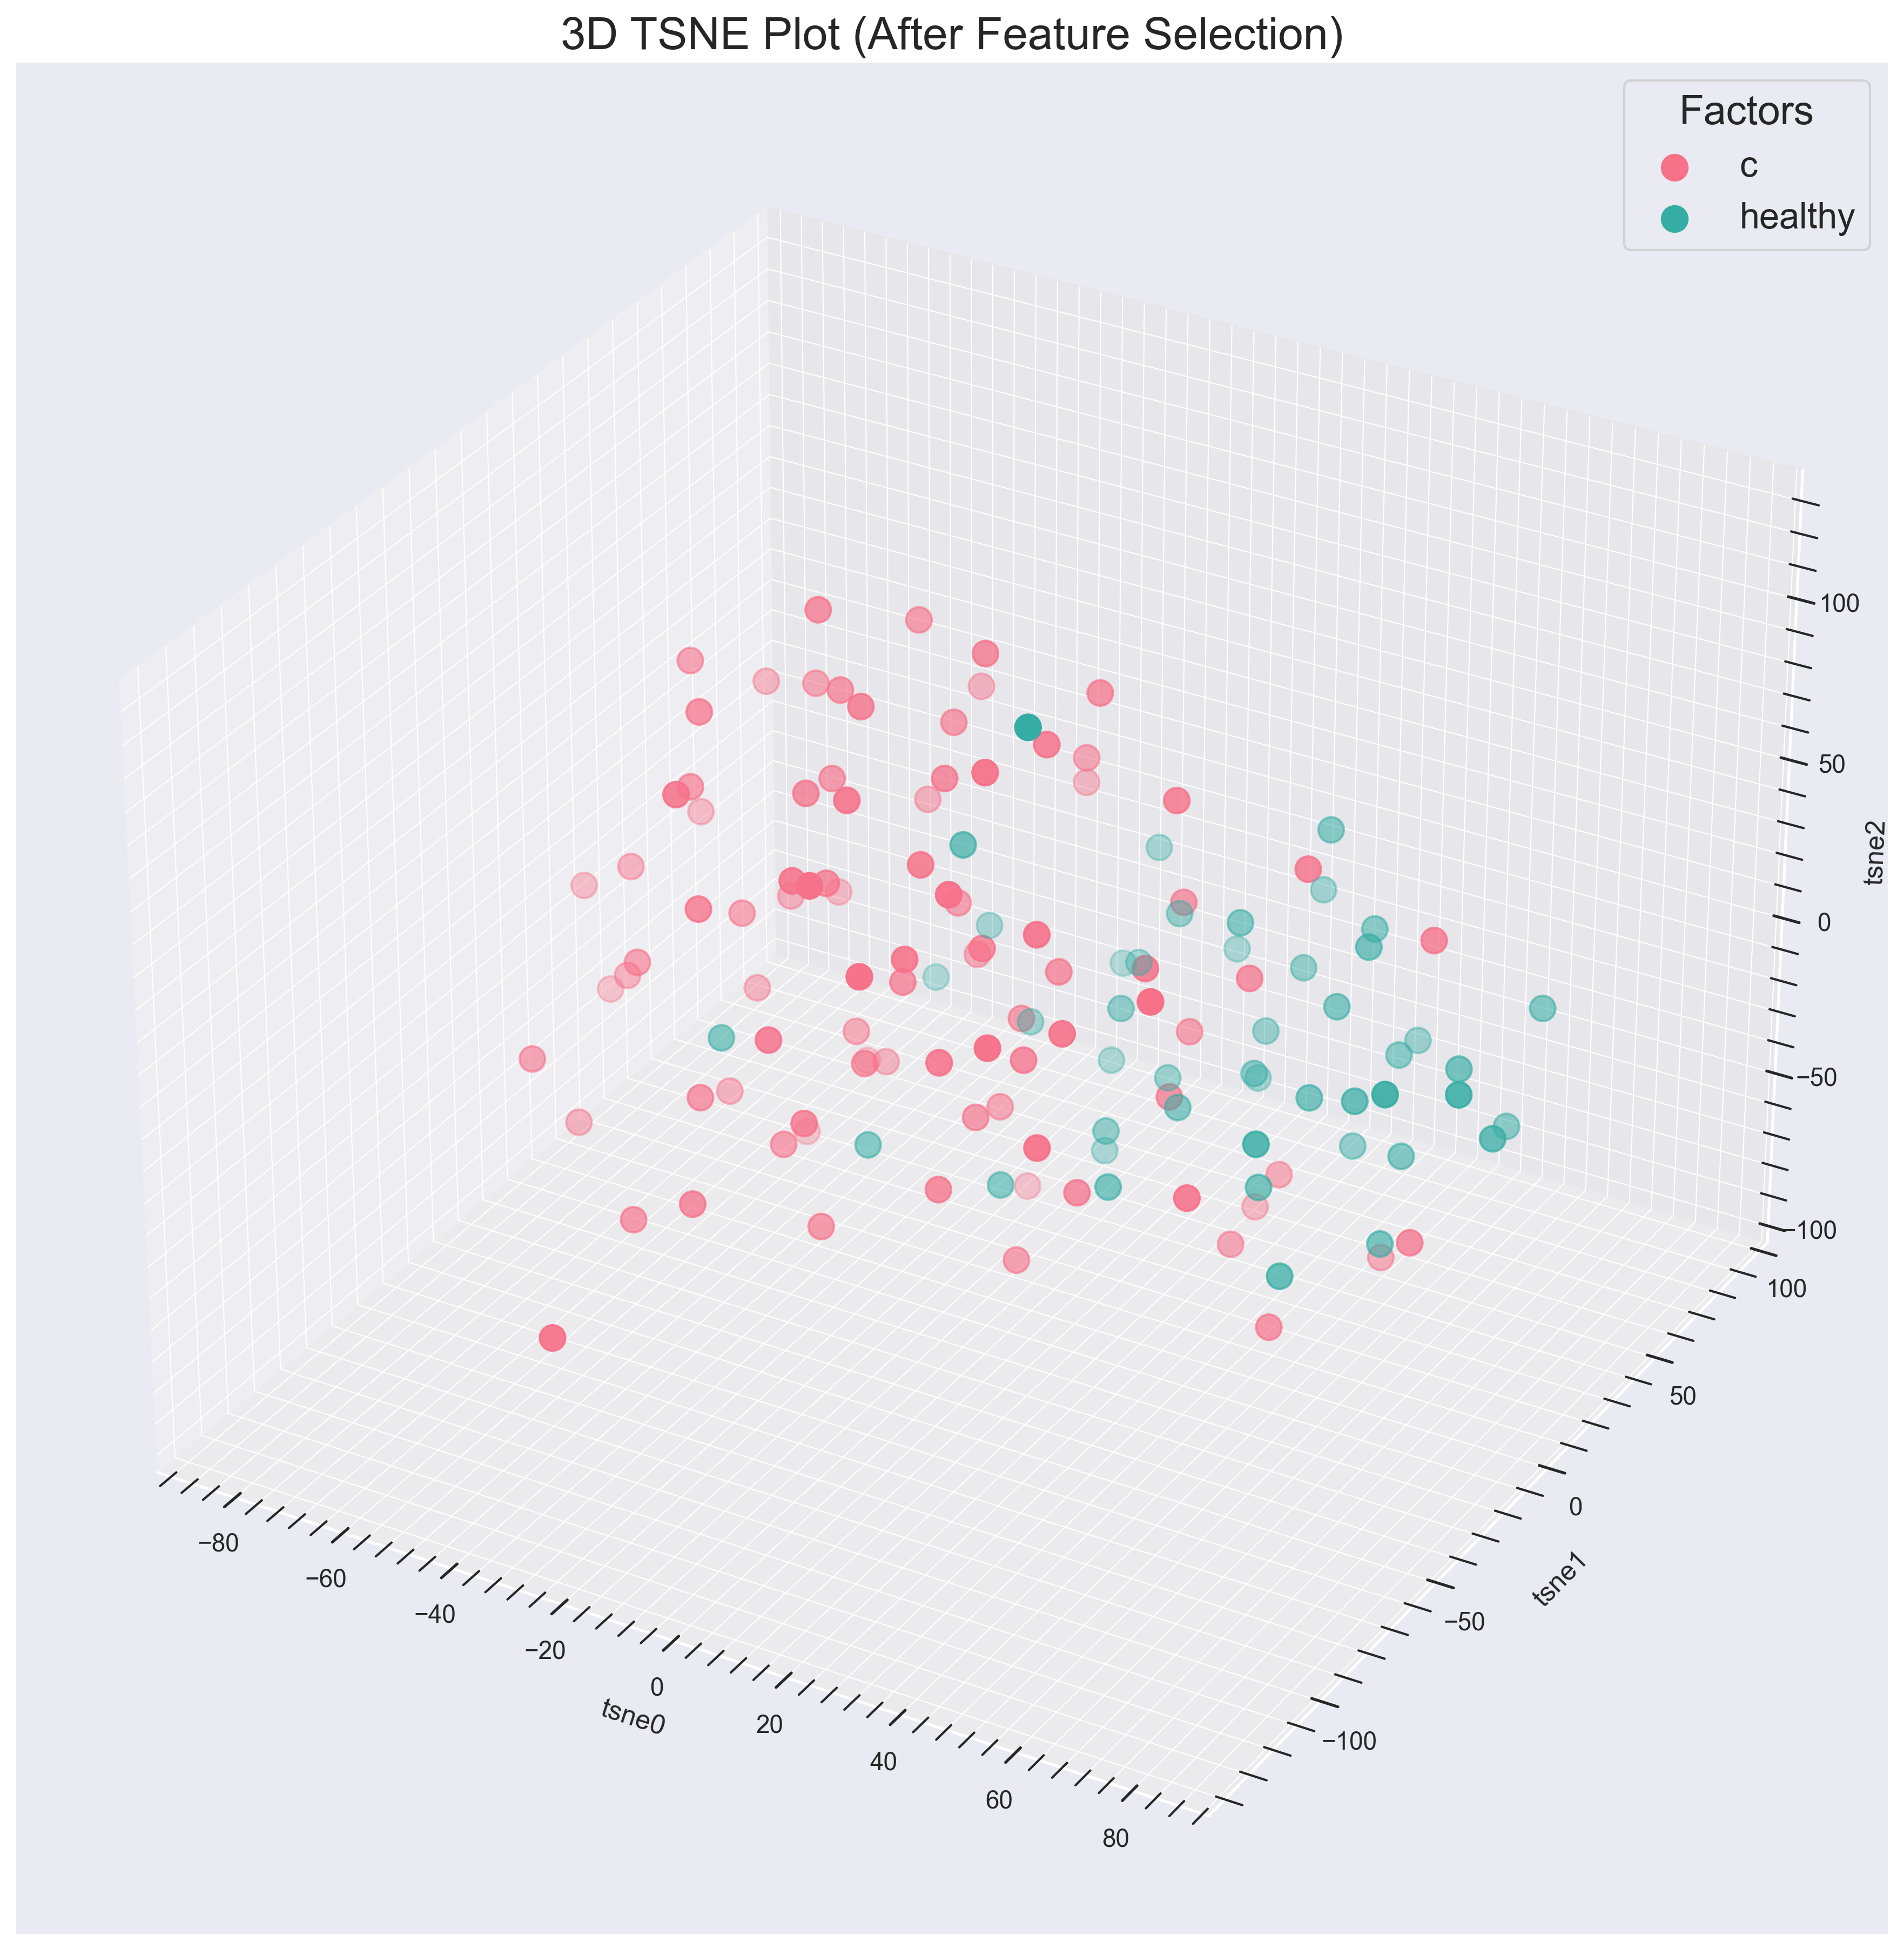
\includegraphics[width=\linewidth]{prostate_cancer_figures/clustering/after_feature_selection/3D_tsne_plot.png}
\caption{3D t-SNE Plot of prostate cancer samples. This non-linear technique visualizes the data by preserving local structures, showing distinct and well-separated clusters for the two groups.}
\label{fig:prostate_tsne}
\end{figure}

\begin{figure}[htbp]
\centering
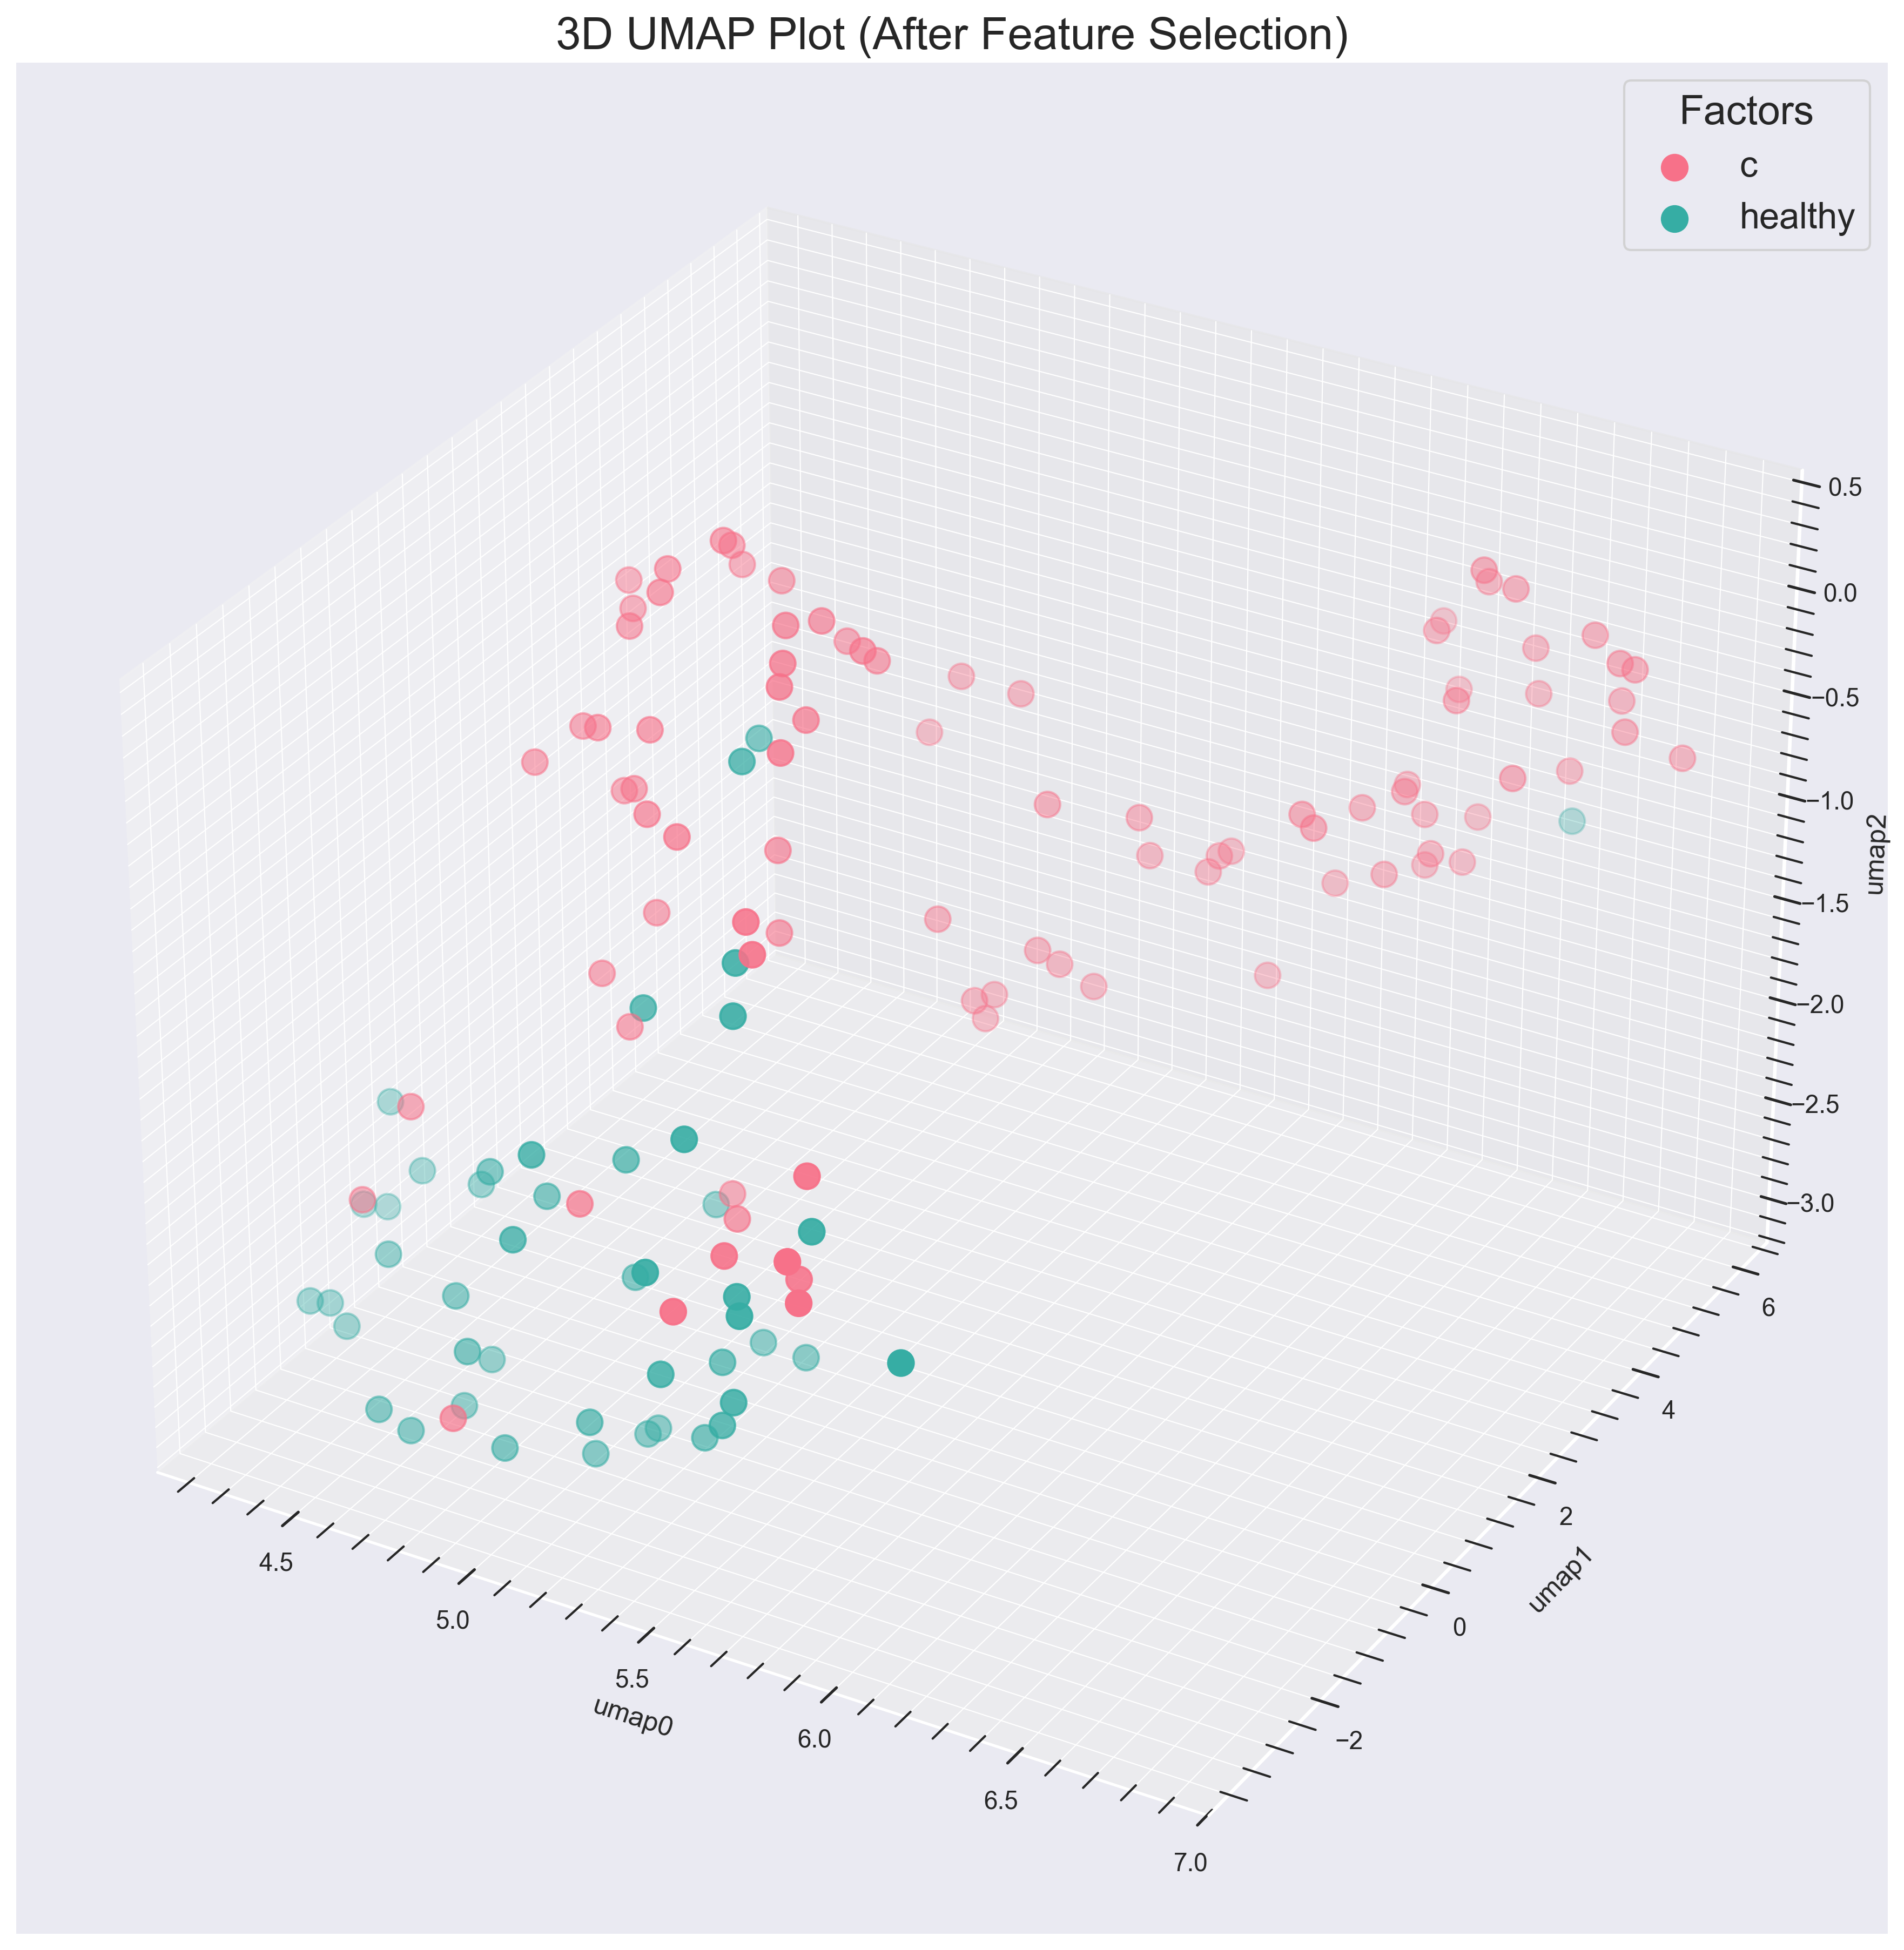
\includegraphics[width=\linewidth]{prostate_cancer_figures/clustering/after_feature_selection/3D_umap_plot.png}
\caption{3D UMAP Plot of prostate cancer samples. UMAP provides a balanced representation of local and global structure, revealing highly compact and clearly separated clusters.}
\label{fig:prostate_umap}
\end{figure}

\paragraph{Classification Analysis and Predictive Model Performance}
To assess the diagnostic potential of the identified biomarker signature, a comprehensive classification analysis was performed using the Biomark tool. Various machine learning models were trained to distinguish between cancer and healthy samples using the transcriptomic profiles. The performance of these models was systematically evaluated with stratified k-fold cross validation and is presented in Table~\ref{tab:all_models_comparison_grouped_v2}. As detailed in Section \ref{sec:feature_selection_mechanism_label}, the analysis was conducted in two stages: first using the "Without Feature Selection" approach on the entire high-dimensional feature set, and subsequently using the "After Feature Selection" approach on a refined subset of the most informative biomarkers. The results clearly demonstrate the strength of the identified biomarker set in building accurate predictive models from omics data. When models were trained on the full dataset, their performance was moderate, reflecting the challenge of learning from noisy, high-dimensional data. However, applying feature selection to focus on identified key biomarkers led to a dramatic and universal improvement in all metrics evaluated for almost every model. The Support Vector Classifier (SVC) emerged as the top-performing model after biomarker selection, achieving an impressive accuracy of 0.94 and a robust F1-score of 0.88. Other models, such as Logistic Regression and the MLP Classifier, also showed excellent performance, with accuracies of 0.92 and 0.90, respectively. This significant boost in predictive power strongly validates the diagnostic relevance of the selected biomarker panel and showcases BioMark's effectiveness in facilitating an end-to-end workflow, from biomarker discovery to the construction of high-performance diagnostic tools.

\begin{table}[h]
\centering
\caption{Classification Model Performance Metrics for \\Prostate Cancer Diagnosis} 
\label{tab:all_models_comparison_grouped_v2}
\begin{tabular}{lcccc}
\toprule
\multicolumn{5}{c}{\textbf{Without Feature Selection}} \\
\midrule
Model  & Accuracy & Precision & Recall & F1-Score \\
\midrule
Logistic Regression& 0.78 & 0.59  & 0.97   & 0.72 \\
Random Forest  & 0.80 & 0.71  & 0.48   & 0.56 \\
XGBClassifier  & 0.82 & 0.72  & 0.61   & 0.66 \\
Decision Tree  & 0.75 & 0.55  & 0.67   & 0.59 \\
Gradient Boosting  & 0.82 & 0.68  & 0.74   & 0.69 \\
CatBoosting Classifier & 0.81 & 0.83  & 0.41   & 0.53 \\
AdaBoost Classifier& 0.81 & 0.72  & 0.60   & 0.62 \\
MLPClassifier  & 0.69 & 0.49  & 0.93   & 0.64 \\
SVC& 0.77 & 0.62  & 0.48   & 0.53 \\
\midrule
\multicolumn{5}{c}{\textbf{After Feature Selection}} \\
\midrule
Model  & Accuracy & Precision & Recall & F1-Score \\
\midrule
Logistic Regression& 0.92 & 0.86  & 0.87   & 0.84 \\
Random Forest  & 0.88 & 0.81  & 0.77   & 0.78 \\
XGBClassifier  & 0.89 & 0.82  & 0.80   & 0.79 \\
Decision Tree  & 0.80 & 0.69  & 0.58   & 0.62 \\
Gradient Boosting  & 0.80 & 0.63  & 0.70   & 0.66 \\
CatBoosting Classifier & 0.90 & 0.79  & 0.87   & 0.82 \\
AdaBoost Classifier& 0.88 & 0.78  & 0.80   & 0.79 \\
MLPClassifier  & 0.90 & 0.80  & 0.90   & 0.83 \\
SVC& 0.94 & 0.88  & 0.90   & 0.88 \\
\bottomrule
\end{tabular}
\end{table}

\subsection{Case Study on Breast Cancer}
This section details the application of the BioMark web tool to a breast cancer biomarker dataset (108 samples, 16,382 features, 'Factors' column for cancer/healthy status), demonstrating the tool's adaptability across varying data characteristics.

\subsubsection{Analysis Results}
\paragraph{Differential Analysis and Biomarker Identification}
To demonstrate BioMark's adaptability, the same comprehensive differential analysis workflow was applied to the breast cancer dataset. The process again combined traditional statistical tests with model-based explainability techniques to uncover the key molecular drivers distinguishing cancer from healthy breast tissue samples.

Statistical analysis with ANOVA (Fig.~\ref{fig:breast_anova_features}) identified biomarkers with the most significant differences in mean expression between the groups. Features such as \textit{VIT}, \textit{SEMA3G}, \textit{PDE2A}, and \textit{KL} ranked highest based on their F-values, establishing their strong statistical relevance in separating the cohorts.

For a more nuanced, interaction-aware perspective, we employed SHAP and LIME to interpret the predictions of a machine learning model. The SHAP Summary Plot (Fig.~\ref{fig:breast_shap_summary}) provides a global overview of the features most impactful to the model. Notably, for top biomarkers like \textit{KL} and \textit{ZHX3}, low expression levels (blue dots) are associated with high positive SHAP values, indicating that their downregulation is a strong predictor of breast cancer. This contrasts with the patterns observed in the prostate cancer dataset and highlights the disease-specific nature of biomarker signatures. The SHAP Heatmap (Fig.~\ref{fig:breast_heatmap}) visualizes this phenomenon across all samples, revealing a clear separation where the cancer cohort (right side) is characterized by patterns of biomarker contributions that are distinct from the healthy cohort (left side).

Instance-level explanations further clarify these relationships. The SHAP Waterfall plots (Fig.~\ref{fig:breast_shap_waterfall}) elegantly contrast the model's reasoning for a healthy versus a cancer sample. For the healthy sample, high expression of \textit{KL} and \textit{ZHX3} strongly contributes to a "healthy" prediction. Conversely, for the cancer sample, low expression of these same biomarkers are the primary drivers of the "cancer" classification. The LIME plot (Fig.~\ref{fig:breast_lime_bar}) offers a similar local validation for a single healthy sample, showing that high expression of \textit{PCYOX1} and appropriate levels of other markers like \textit{ABCA6} and \textit{DENND2D} solidified its correct classification. By integrating these multi-faceted insights, BioMark successfully identified significant biomarkers like \textit{DENND2D}, \textit{PYROXD2}, and \textit{DPT}, and elucidated their complex predictive roles, underscoring the platform's power in extracting context-rich biological information from diverse datasets.

% FIGURE DEFINITIONS (Breast Cancer)

\begin{figure}[htbp]
\centering
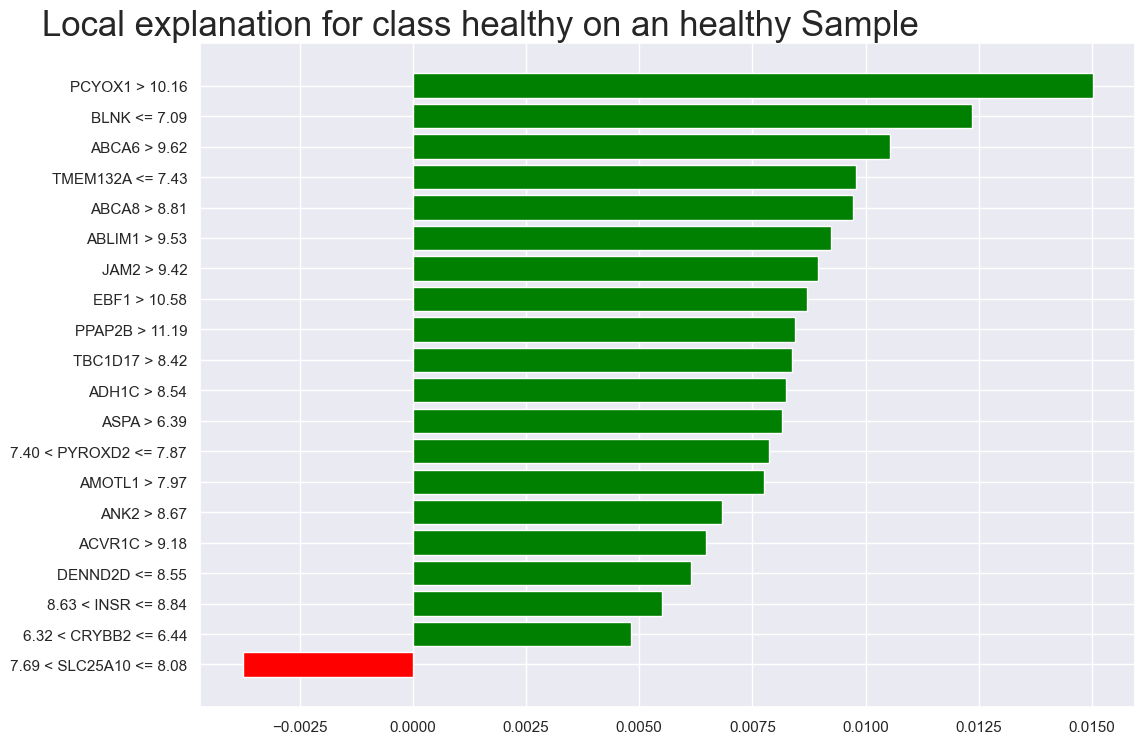
\includegraphics[width=\linewidth]{breast_cancer_figures/differential/lime_local_explanation_plot_healthy.png}
\caption{LIME plot illustrating top contributing biomarkers for a single breast cancer sample prediction.}
\label{fig:breast_lime_bar}
\end{figure}

\begin{figure}[htbp]
\centering
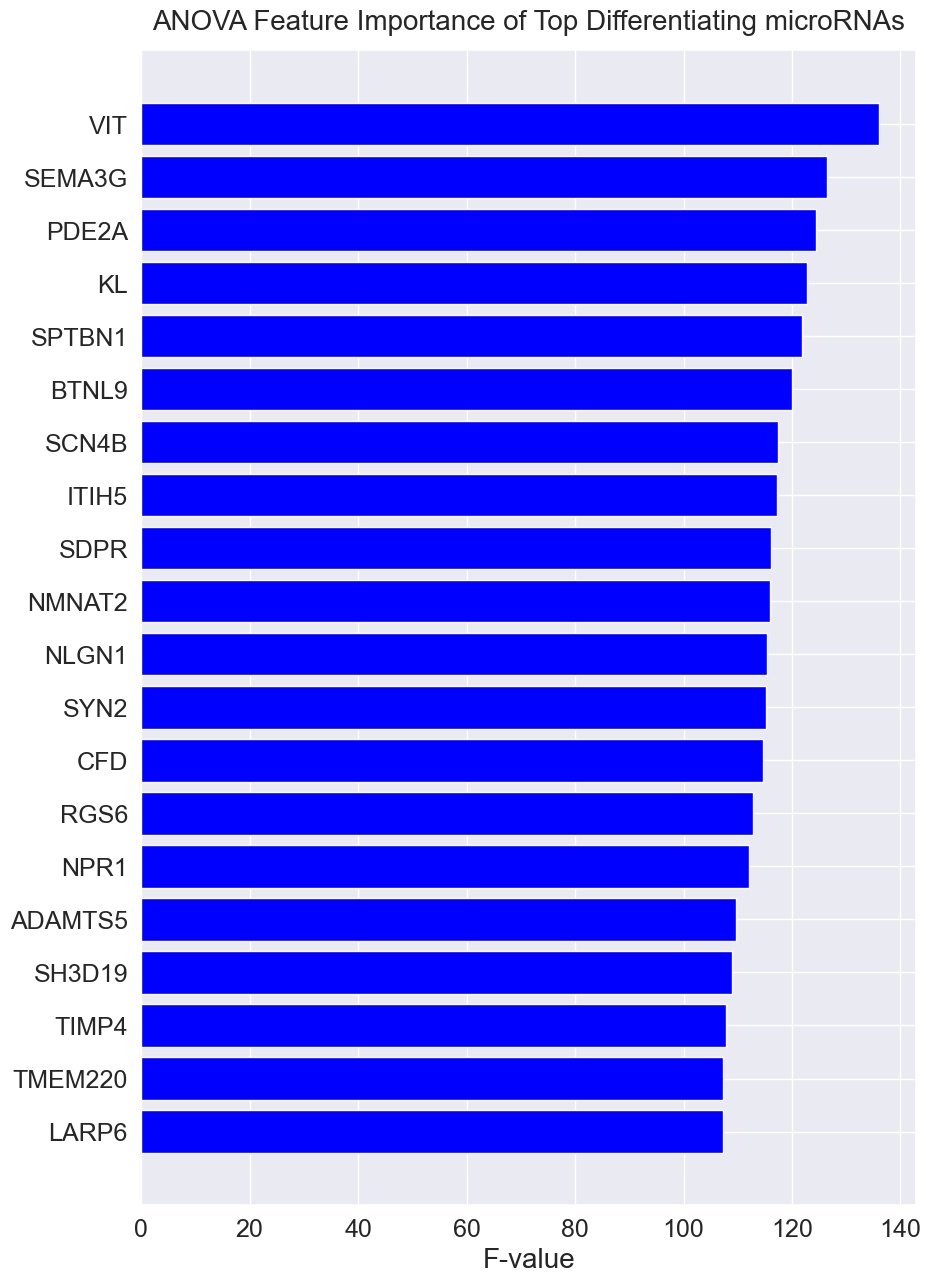
\includegraphics[width=\linewidth]{breast_cancer_figures/differential/anova_features_plot.png}
\caption{The most discriminative biomarkers detected by the ANOVA test in the breast cancer dataset, ranked by F-value.}
\label{fig:breast_anova_features}
\end{figure}

\begin{figure}[htbp]
\centering
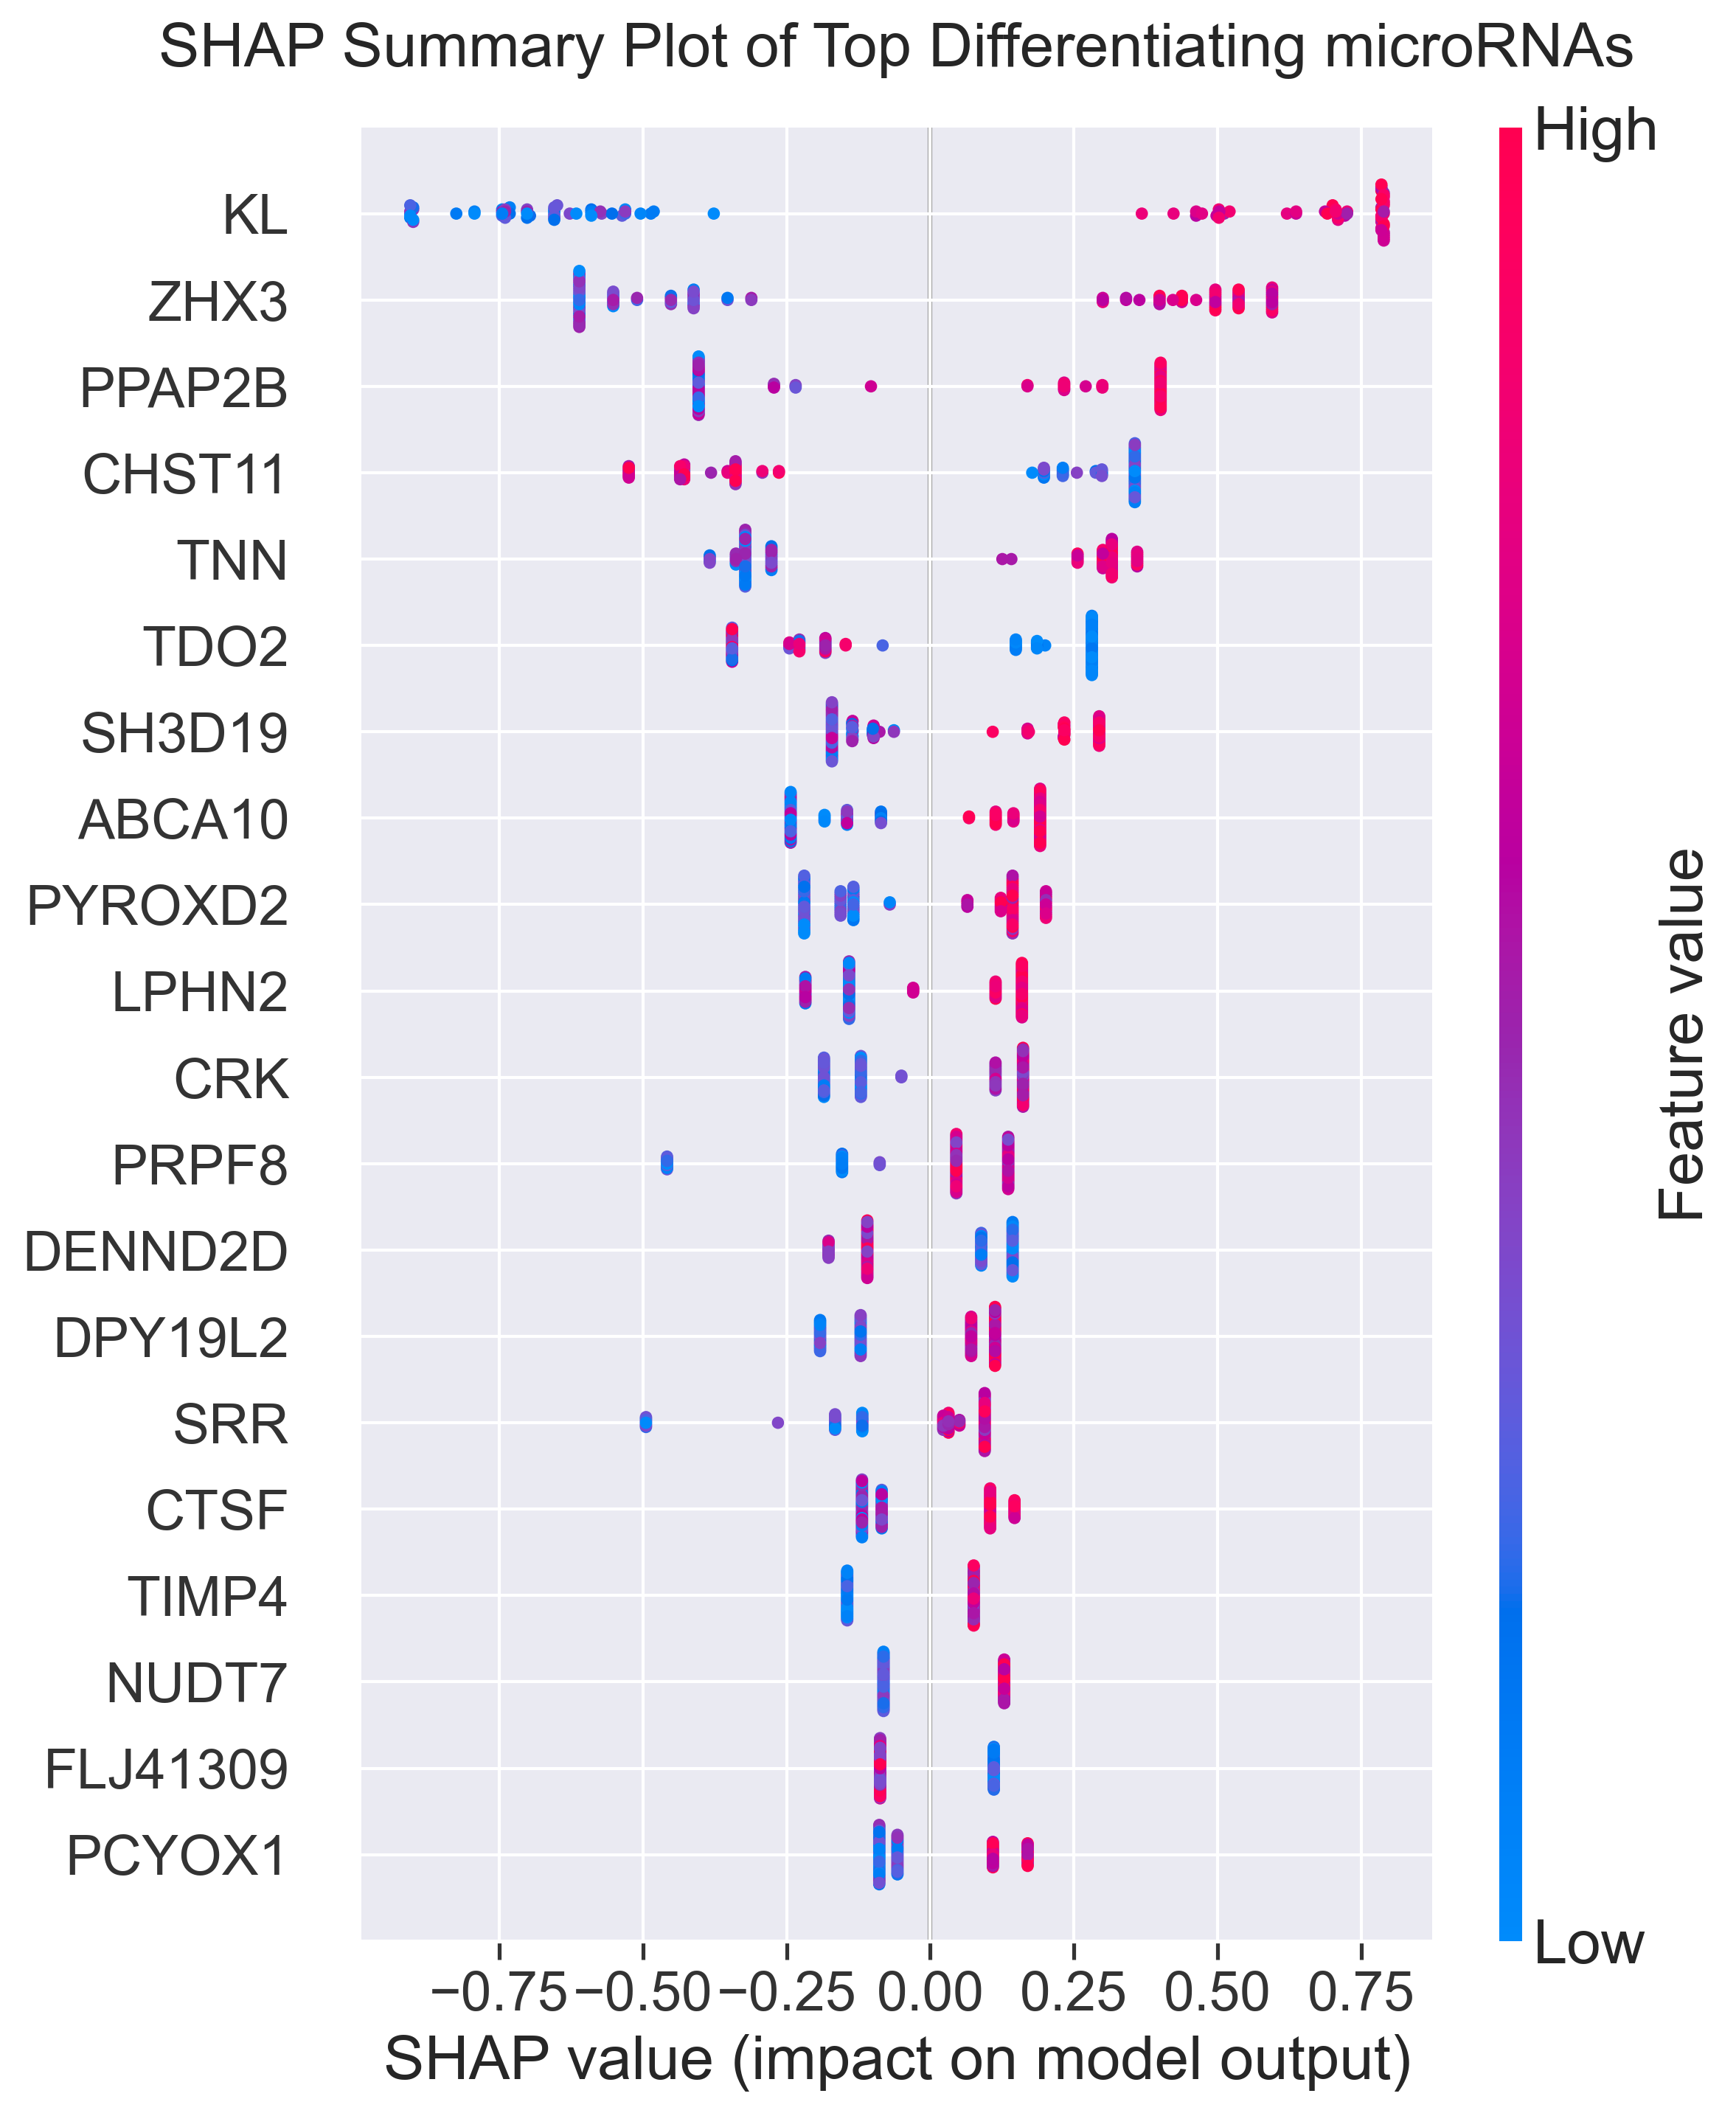
\includegraphics[width=0.9\linewidth]{breast_cancer_figures/differential/shap_summary_plot_healthy_and_c.png}
\caption{SHAP Summary Plot for Breast Cancer Differential Analysis. This plot illustrates the global impact of top biomarkers, showing for instance that low expression (blue) of KL and ZHX3 pushes the prediction towards cancer (positive SHAP value).}
\label{fig:breast_shap_summary}
\end{figure}

\begin{figure}[htbp]
\centering
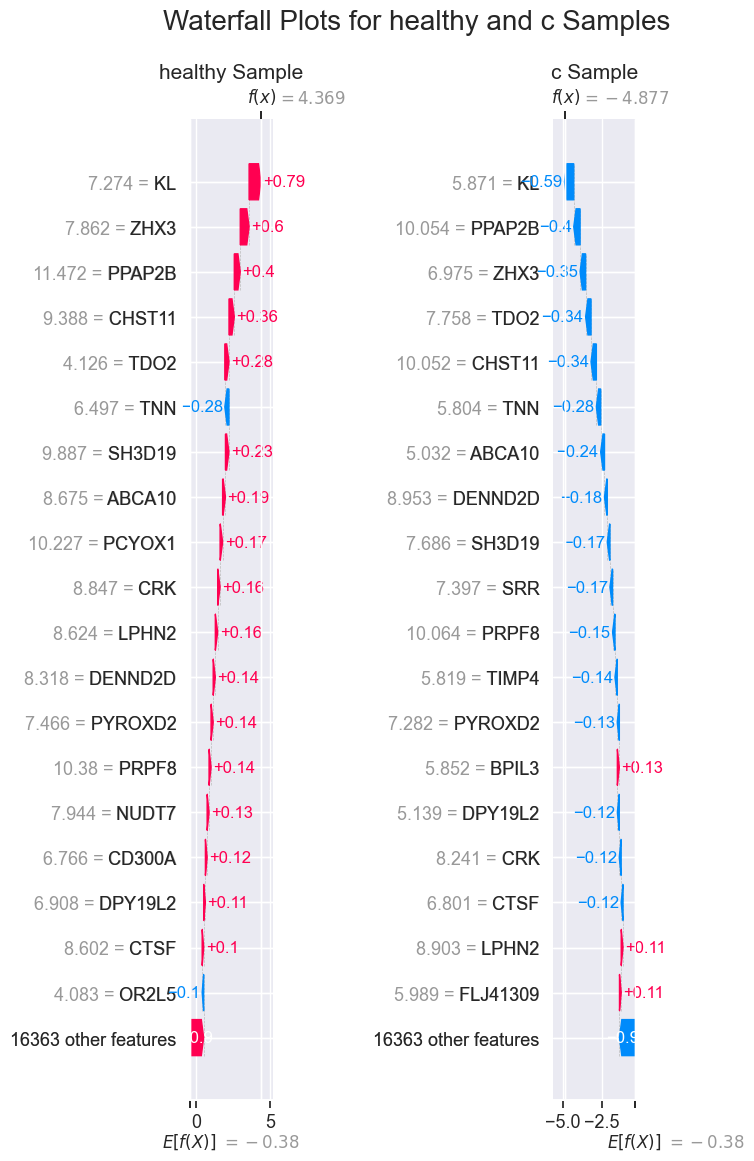
\includegraphics[width=0.8\linewidth]{breast_cancer_figures/differential/shap_waterfall_subplots_healthy_and_c.png}
\caption{SHAP Waterfall plots for Breast Cancer, contrasting the model's prediction for a healthy sample (left) and a cancer sample (right) by showing individual biomarker contributions.}
\label{fig:breast_shap_waterfall}
\end{figure}

\begin{figure}[!htbp]
\centering
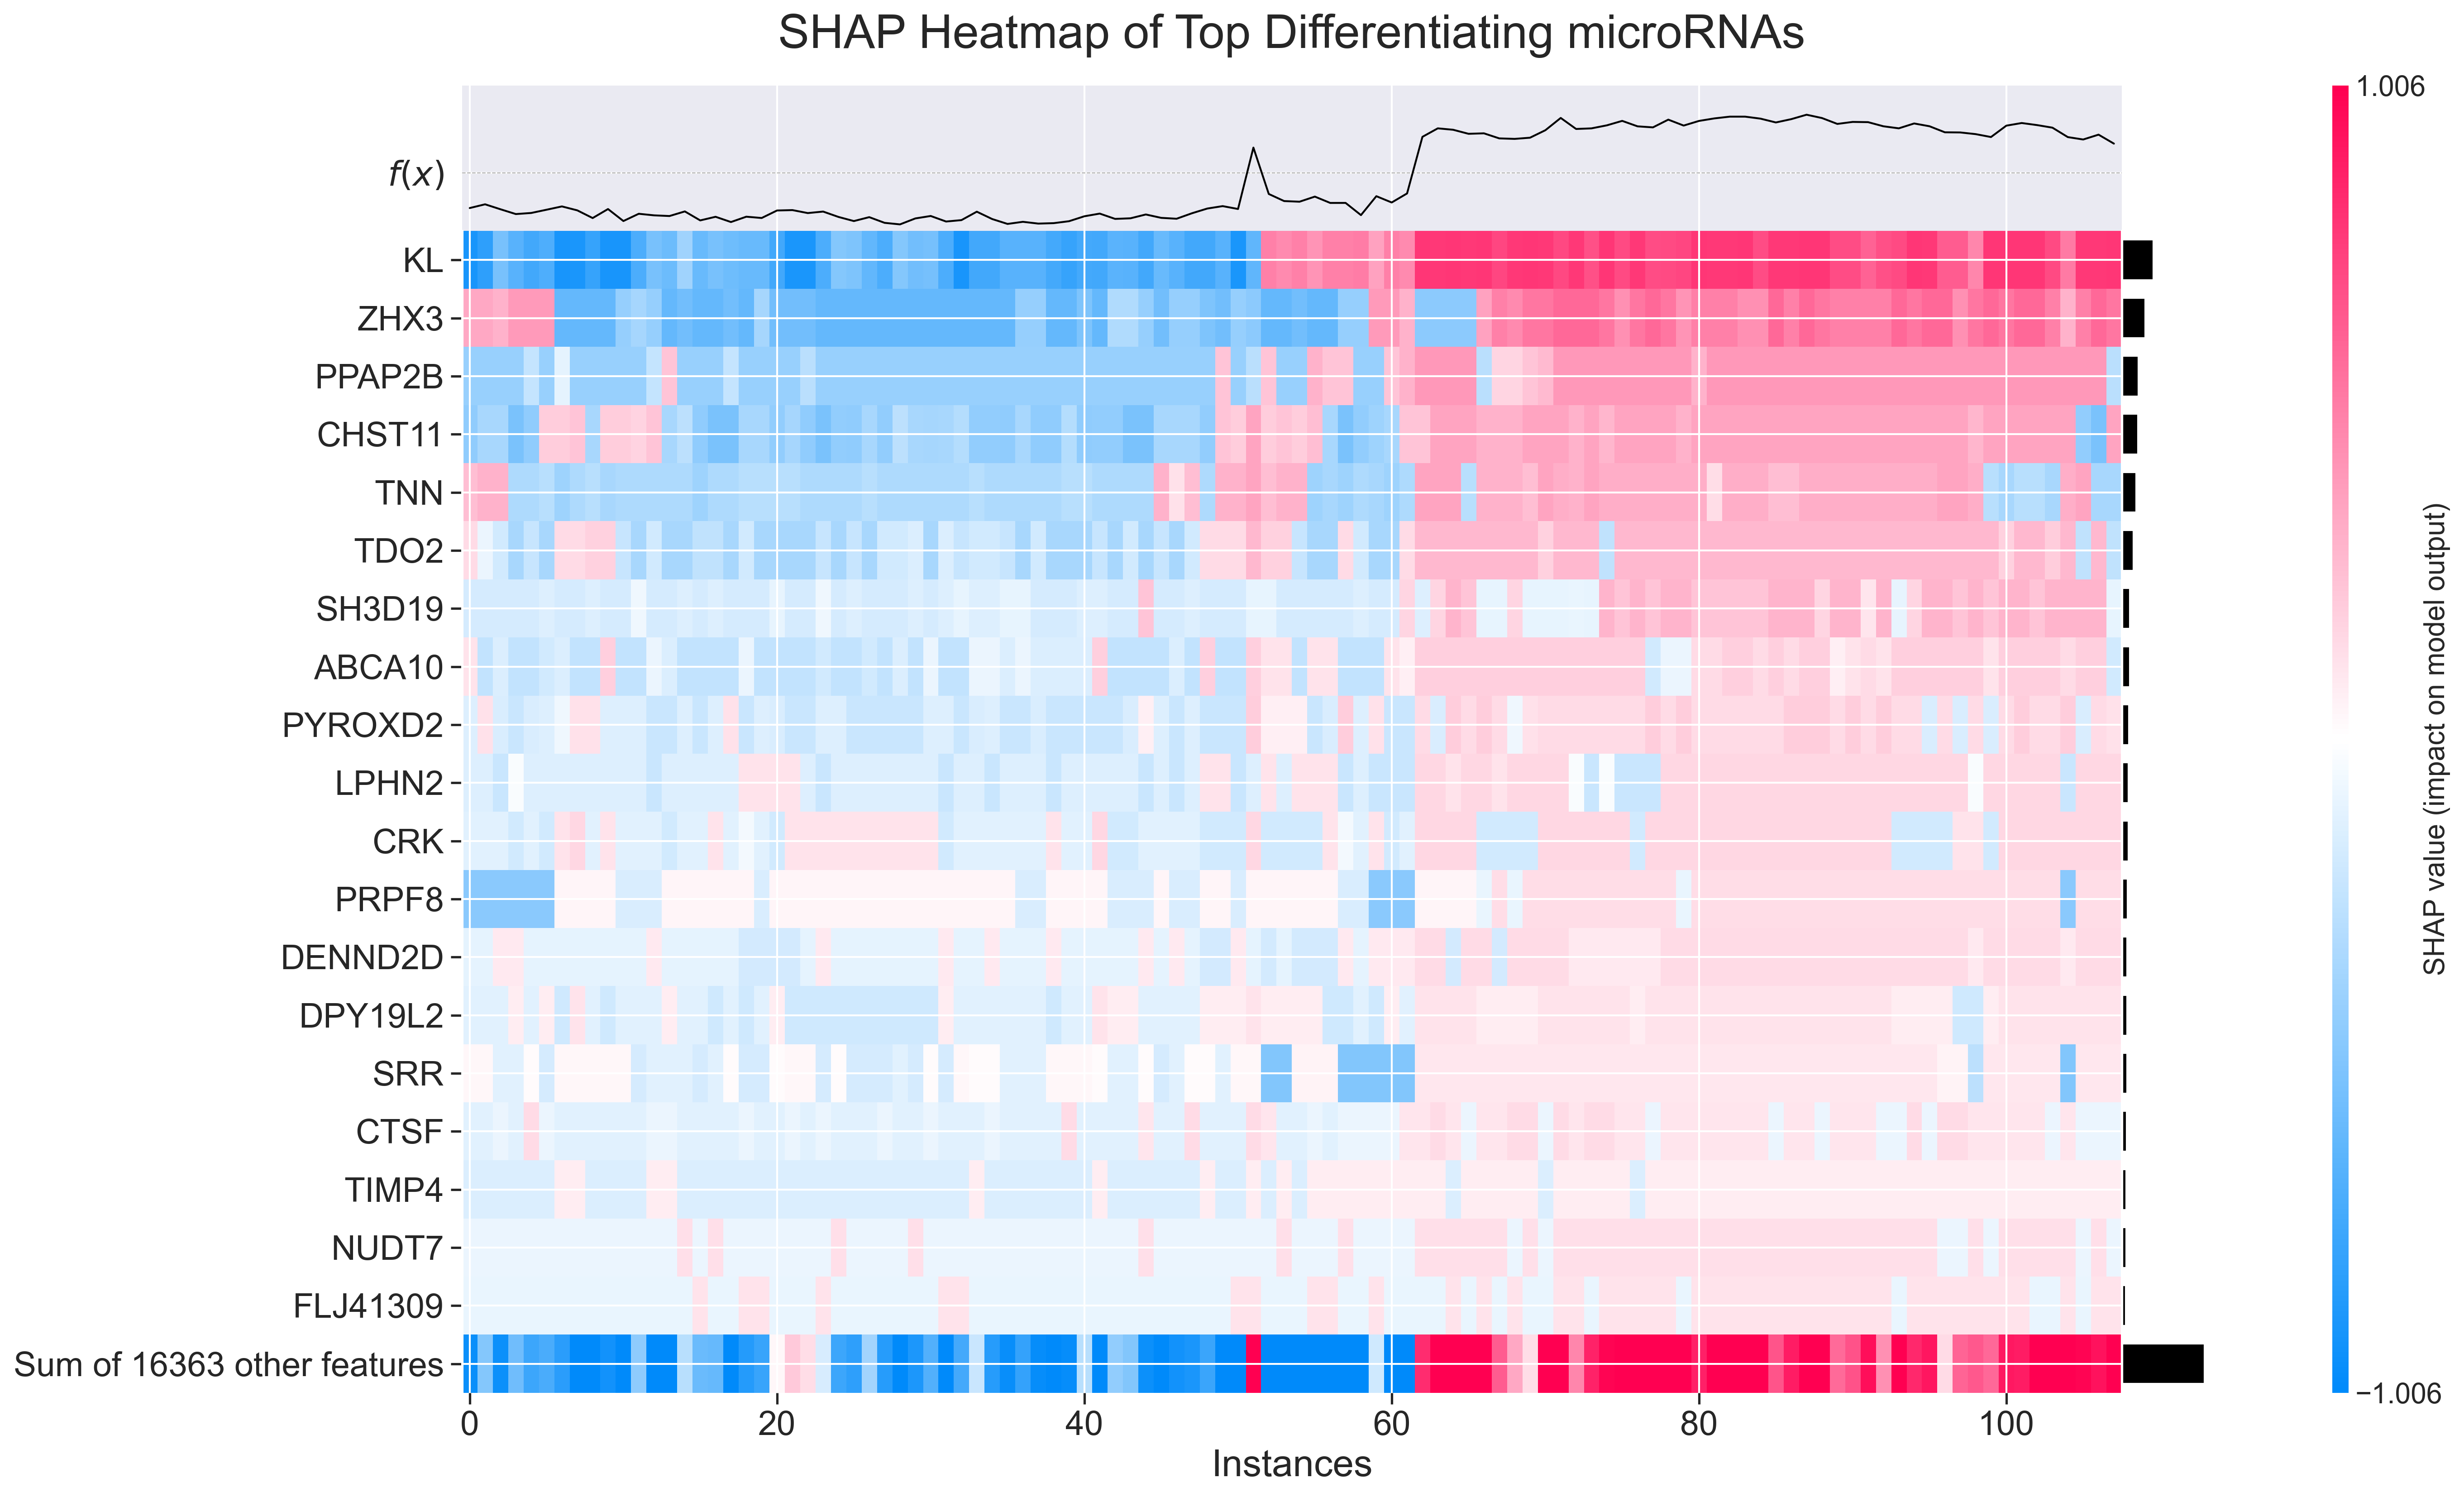
\includegraphics[width=\linewidth]{breast_cancer_figures/differential/shap_heatmap_plot_healthy_and_c.png}
\caption{Heatmap of Top Differentiating Biomarkers in Breast Cancer. It displays the SHAP values for each sample, revealing distinct explanatory patterns between the healthy and cancer cohorts.}
\label{fig:breast_heatmap}
\end{figure}

\begin{figure}[htbp]
\centering
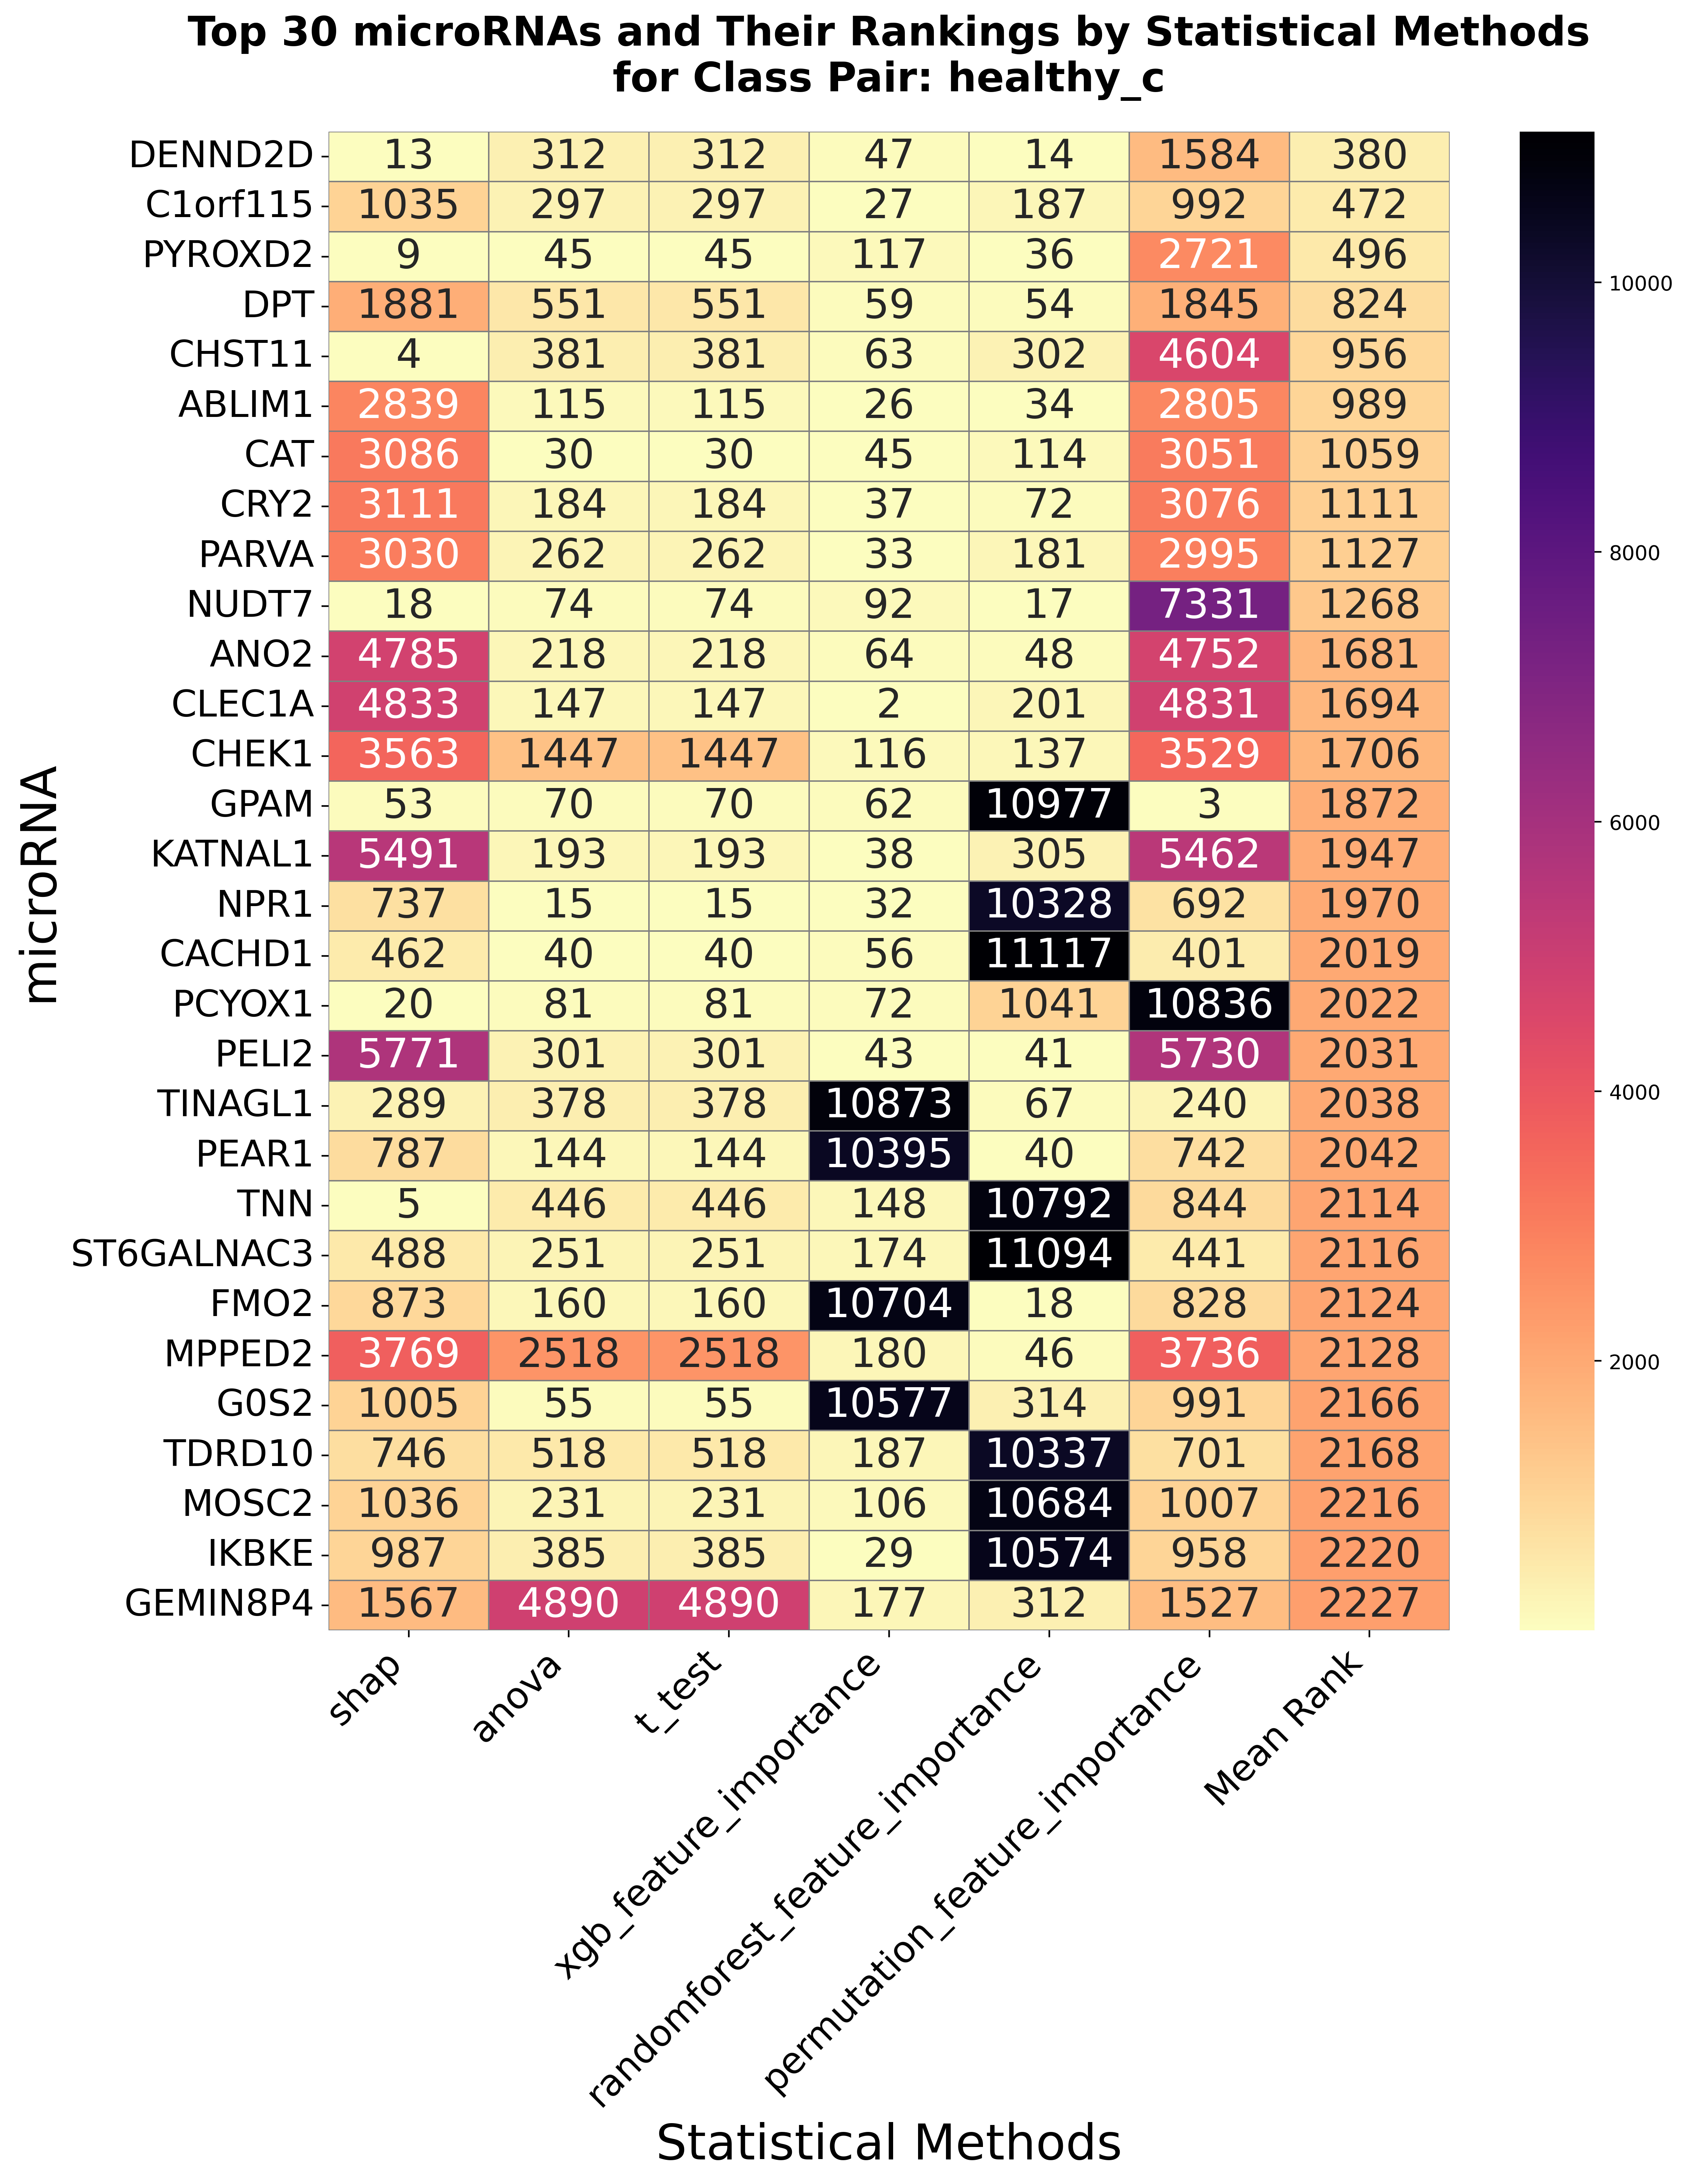
\includegraphics[width=\linewidth]{breast_cancer_figures/summary/summary_of_statistical_methods_plot.png}
\caption{Consolidated ranking of the top 20 differentiating biomarkers in Breast Cancer. The plot summarizes feature importance scores from multiple methods (SHAP, LIME, ANOVA, etc.) to provide a robust consensus list of molecules distinguishing cancer samples from healthy controls.}
\label{fig:breast_biomarker_summary}
\end{figure}

\subsubsection{Literature-Based Validation of Identified Biomarkers}

To further validate our tool's performance, the biomarkers identified in the breast cancer dataset were cross-referenced with published findings, revealing a strong overlap with established research across diverse biological functions. BioMark successfully flagged multiple genes with confirmed roles in breast cancer pathology. For example, \textbf{DPT} (Dermatopontin) is a known tumor suppressor whose downregulation is linked to malignancy \cite{DPT_suppressor_2023}. \textbf{IKBKE} and \textbf{PARVA} were also identified, and both are documented to promote invasion and metastasis \cite{IKBKE_metastasis_2022, PARVA_metastasis_2019}. Additionally, our tool prioritized \textbf{CHEK1}, a crucial marker in triple-negative breast cancer \cite{CHEK1_TNBC_2022}; \textbf{MPPED2}, a tumor suppressor silenced by hypermethylation \cite{MPPED2_suppressor_2019}; and \textbf{CRY2}, a circadian clock gene whose low expression correlates with aggressiveness and poor survival \cite{CRY2_circadian_2015}. The congruence between BioMark's automated analysis and this broad spectrum of manually curated literature findings powerfully underscores the tool's reliability and precision. The identification of less-studied features like \textit{PYROXD2} further highlights its capacity to pinpoint novel candidates worthy of future research.


\paragraph{Clustering Analysis}
The clustering analysis pipeline was subsequently applied to the breast cancer dataset to evaluate its inherent structure and the separability of the cancer and healthy groups. Following the protocol detailed in Section \ref{sec:feature_selection_mechanism_label}, PCA, t-SNE, and UMAP visualizations were generated after feature selection. In striking contrast to the prostate cancer results, the breast cancer samples exhibited a greater degree of inter-group similarity, making their separation more challenging and highlighting the varying complexity of different biological datasets. 

The PCA plot (Fig.~\ref{fig:breast_pca}) revealed only a partial separation between the cancer and healthy samples. While a general trend is visible, there is significant overlap between the two groups, indicating that linear dimensionality reduction is not sufficient to fully distinguish them based on the selected biomarker signature. Similarly, the t-SNE analysis (Fig.~\ref{fig:breast_tsne}), which focuses on local data structure, also resulted in a largely mixed distribution of samples, failing to resolve them into distinct clusters.

However, the UMAP analysis proved to be the most effective method for this more complex dataset (Fig.~\ref{fig:breast_umap}). Despite the challenges, UMAP successfully partitioned the majority of the samples into two discernible clusters, one predominantly composed of healthy samples and the other of cancer samples. This demonstrates UMAP's strength in preserving a more meaningful balance of local and global data structure, allowing it to find patterns that other methods could not. The ability of BioMark to still uncover underlying data structures, even in a dataset with less distinct separation, underscores its utility for patient stratification and highlights the importance of having multiple clustering algorithms available to tackle biological data of varying complexity.

% FIGURE DEFINITIONS (Breast Cancer Clustering)

\begin{figure}[htbp]
\centering
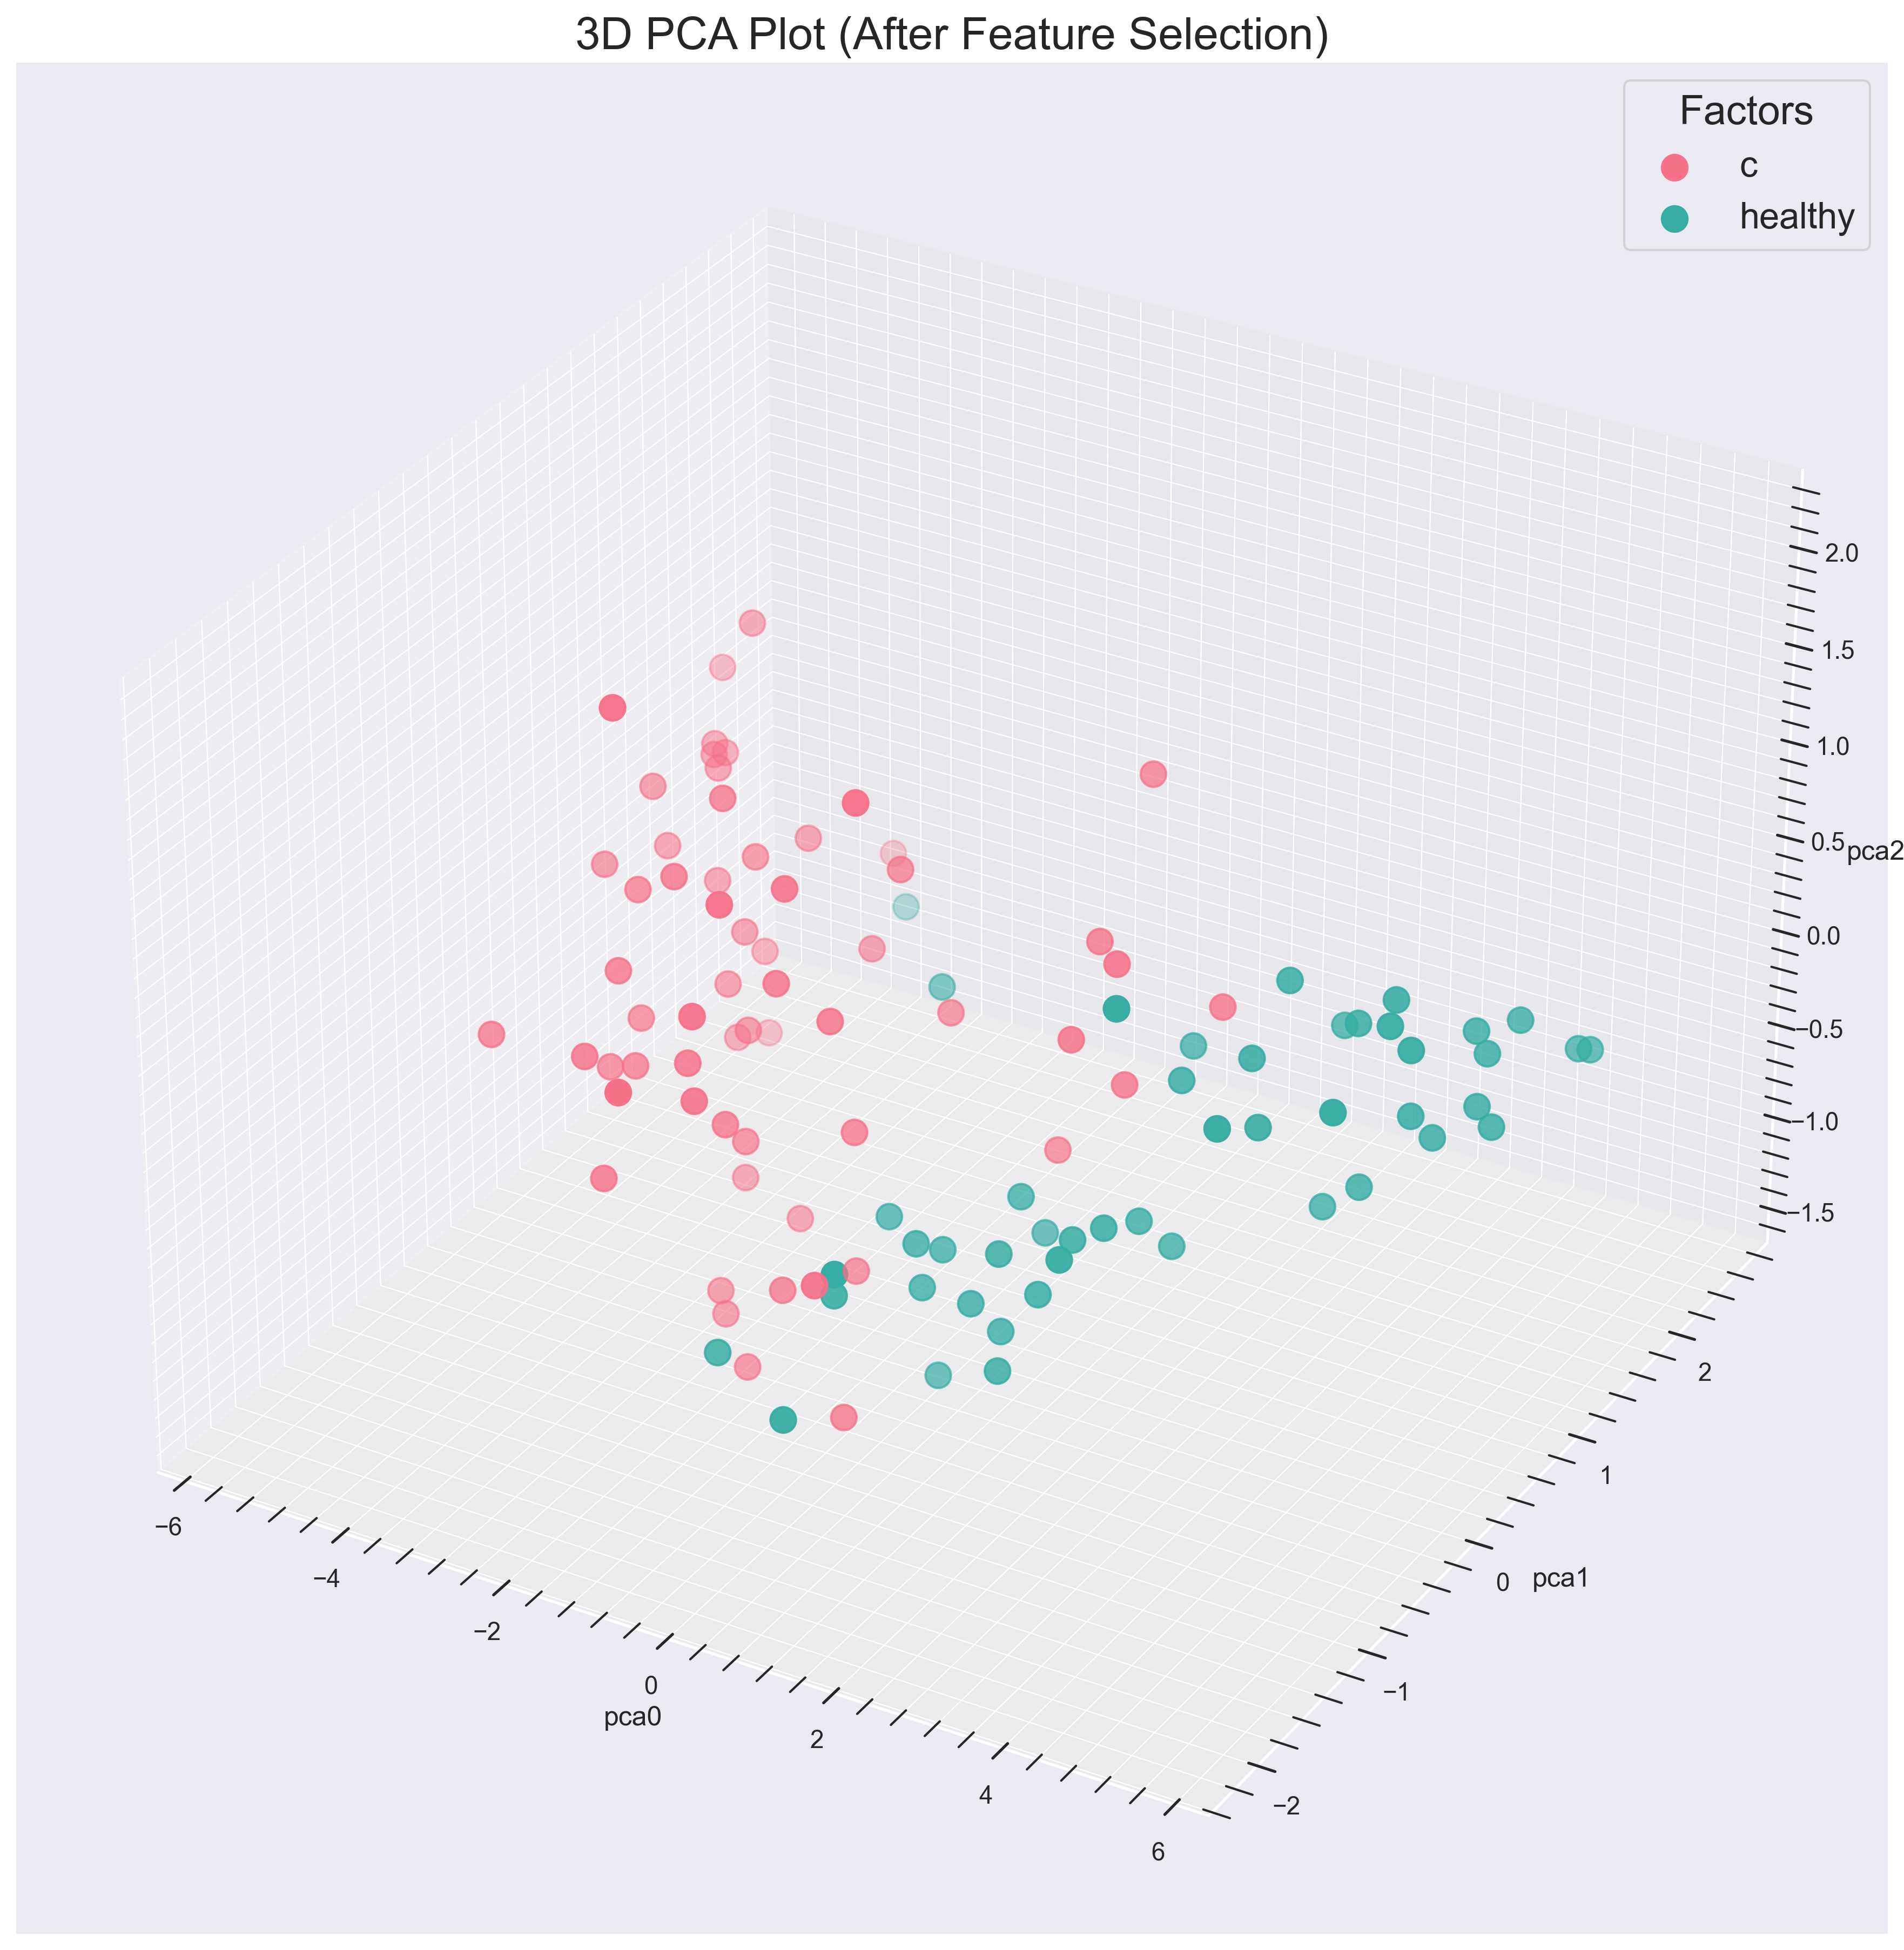
\includegraphics[width=\linewidth]{breast_cancer_figures/clustering/after_feature_selection/3D_pca_plot.png}
\caption{3D PCA Plot for Breast Cancer samples. The visualization shows a partial separation with significant overlap between healthy (teal) and cancer (pink) samples.}
\label{fig:breast_pca}
\end{figure}

\begin{figure}[htbp]
\centering
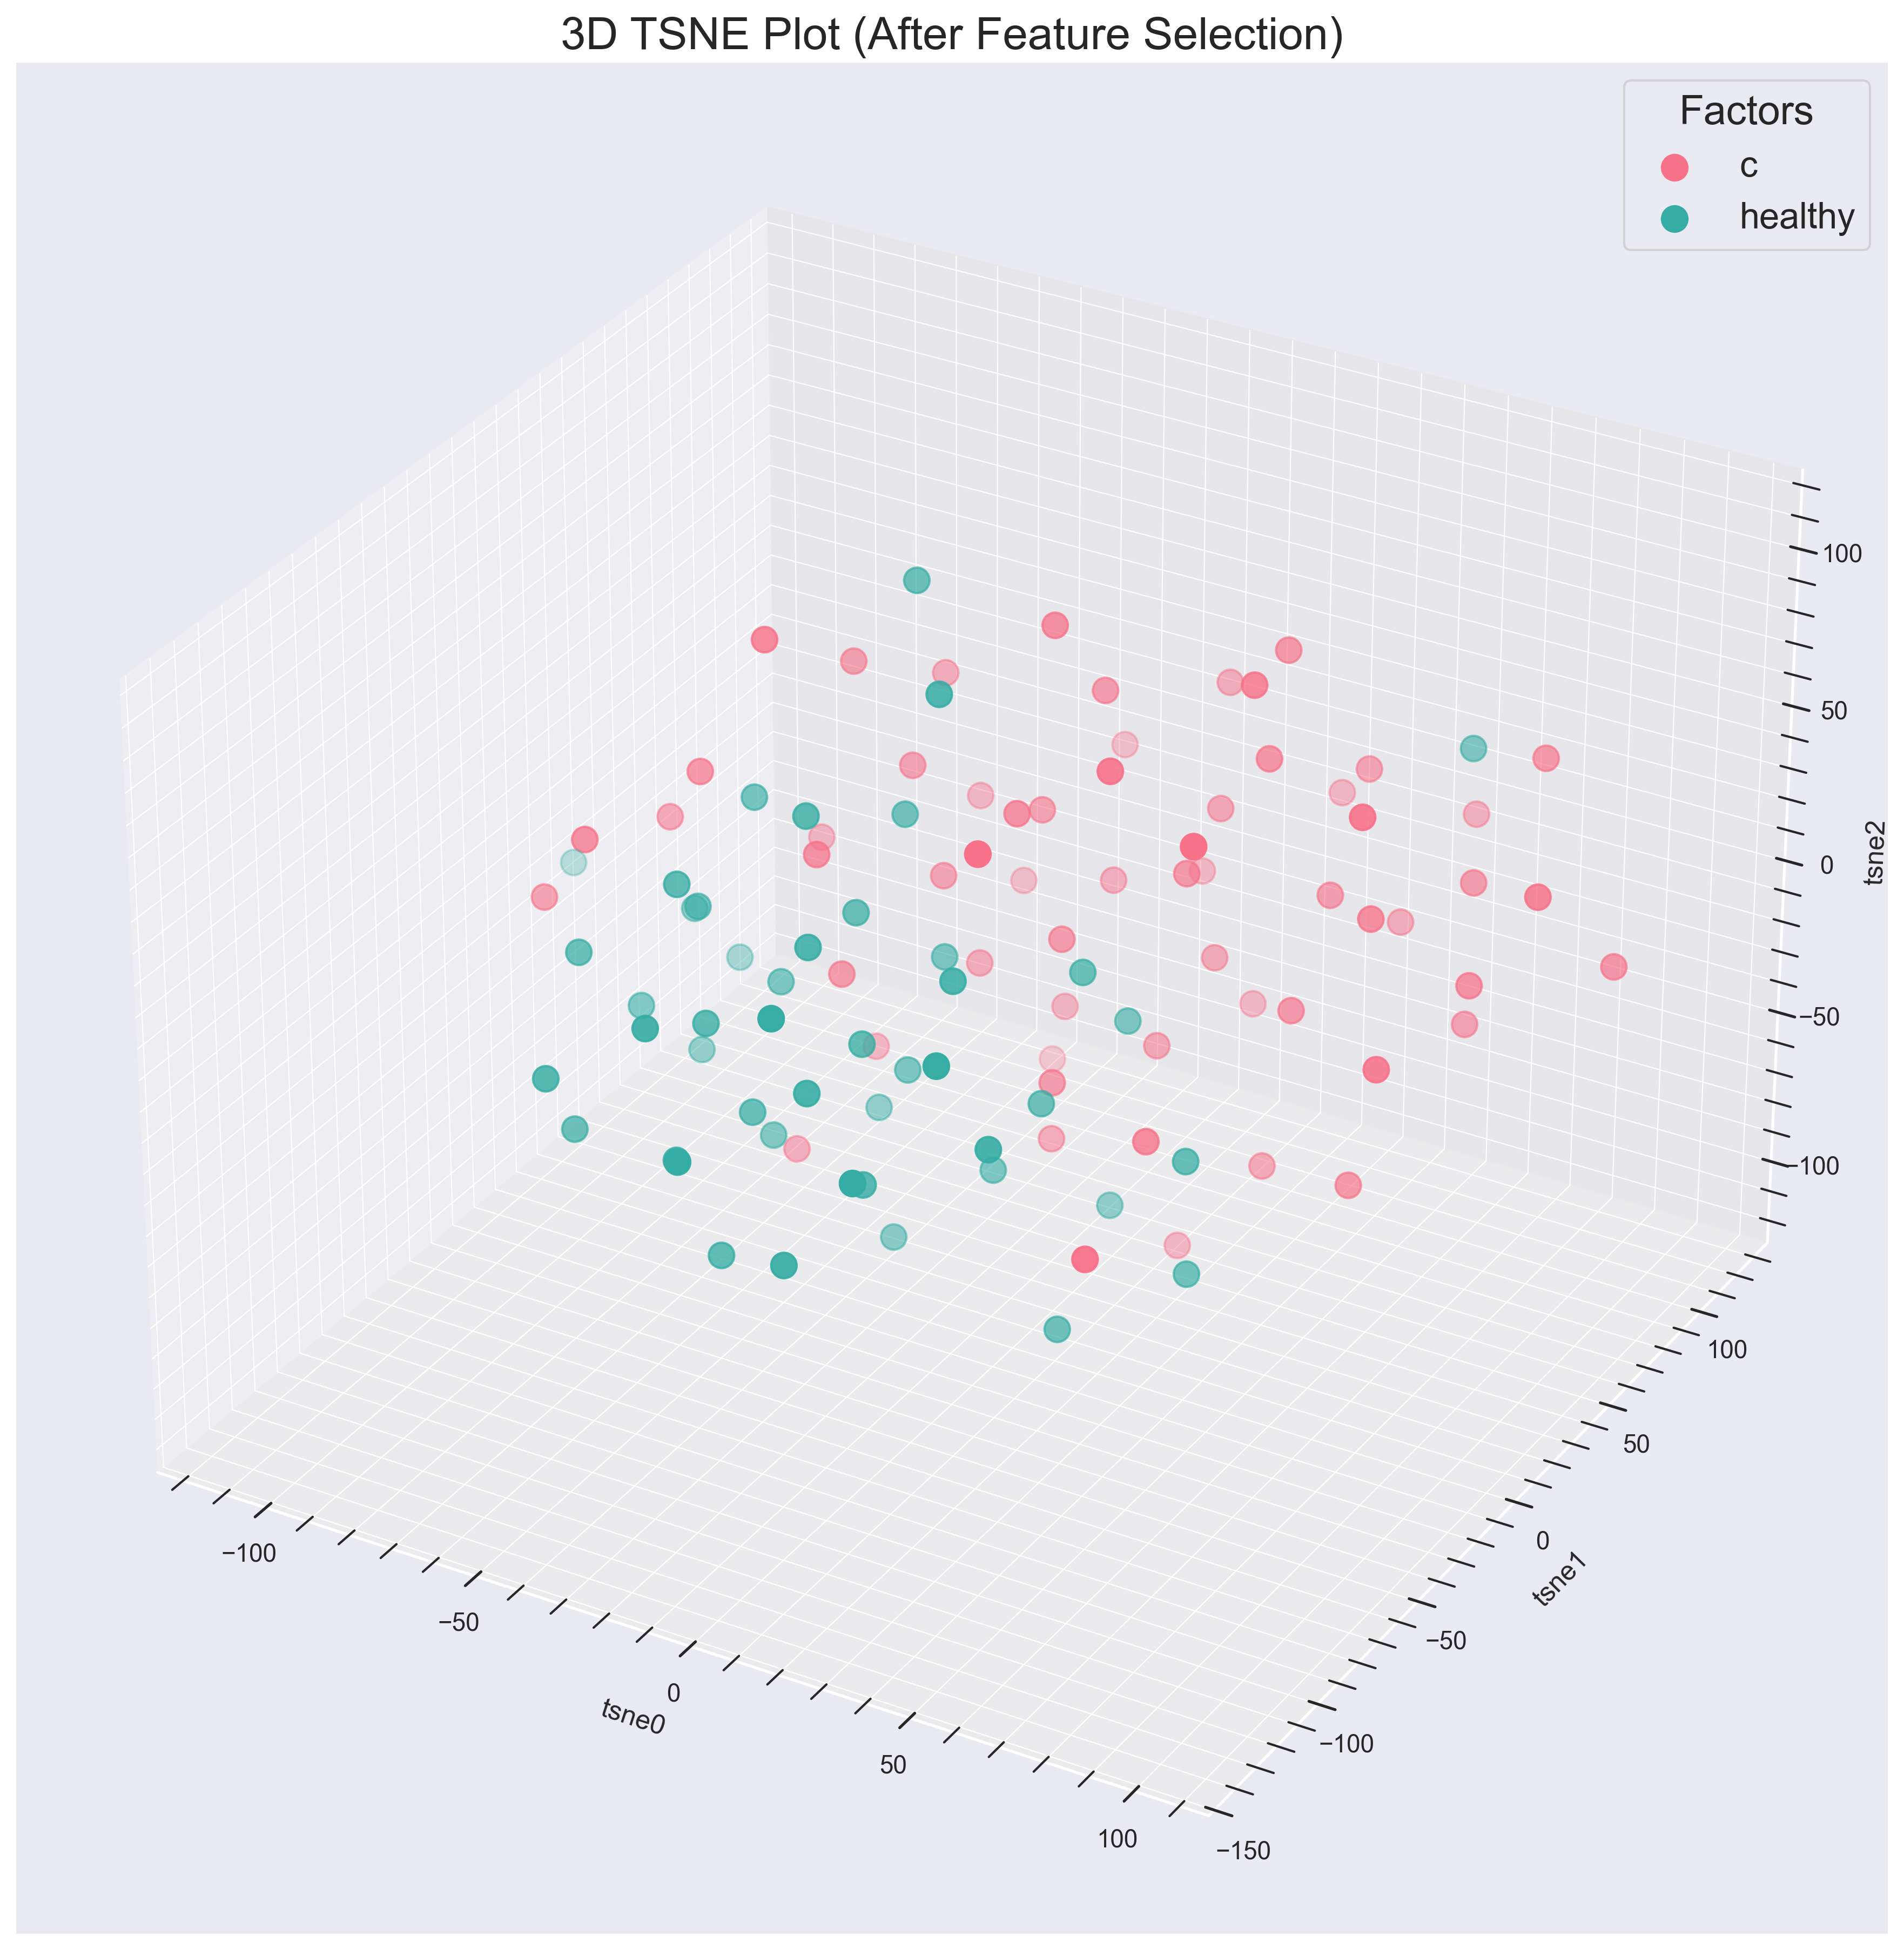
\includegraphics[width=\linewidth]{breast_cancer_figures/clustering/after_feature_selection/3D_tsne_plot.png}
\caption{3D t-SNE Plot for Breast Cancer samples. The two groups remain largely intermingled, indicating a high degree of non-linear similarity.}
\label{fig:breast_tsne}
\end{figure}

\begin{figure}[htbp]
\centering
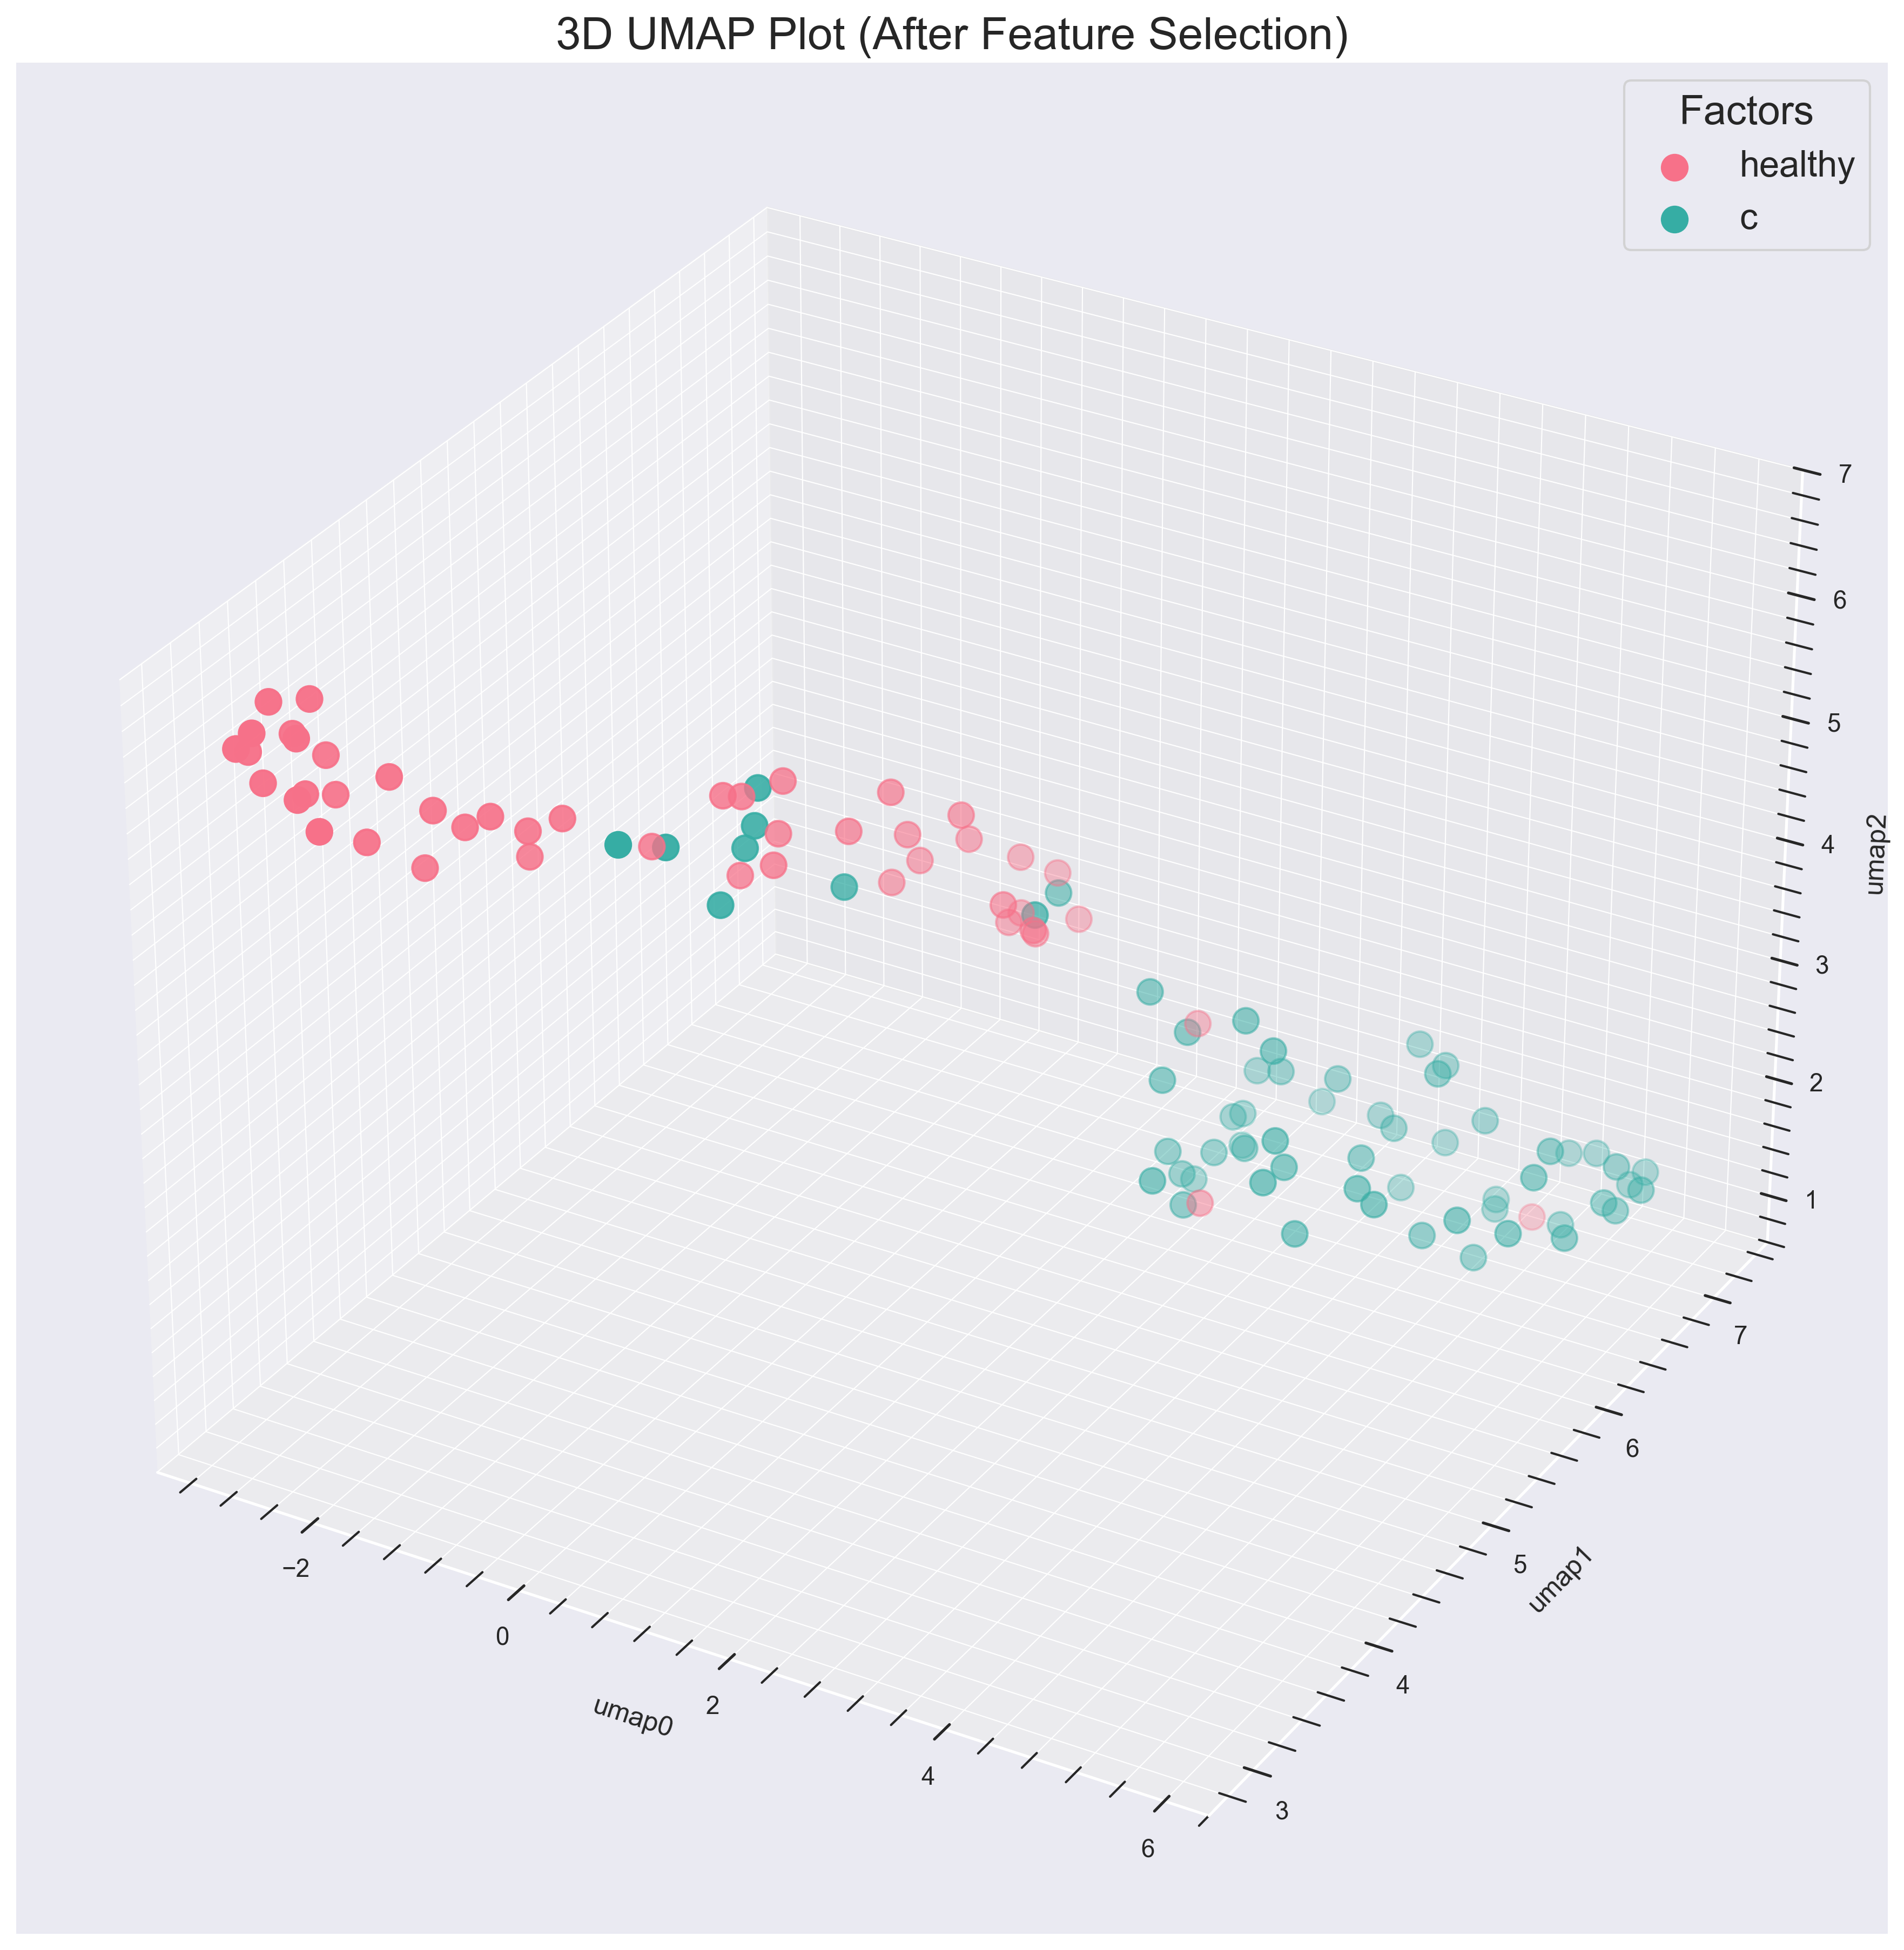
\includegraphics[width=\linewidth]{breast_cancer_figures/clustering/after_feature_selection/3D_umap_plot.png}
\caption{3D UMAP Plot for Breast Cancer samples. UMAP achieves the best separation for this dataset, resolving the samples into two largely distinct clusters.}
\label{fig:breast_umap}
\end{figure}


\paragraph{Classification Analysis and Predictive Model Performance}
Predictive models for breast cancer diagnosis were trained using the same array of machine learning algorithms as for prostate cancer, with their performance evaluated through cross-validation. As with the prostate cancer analysis, model performance was compared between the "Without Feature Selection" approach (using the full feature set) and the "After Feature Selection" approach (using the refined biomarker subset), summarized in Table~\ref{tab:all_models_comparison_grouped}. In contrast to the prostate cancer case, a couple of models (i.e., LR and SVC) for breast cancer performed strongly even without feature selection, suggesting a robust initial biomarker signature. However, the application of feature selection was still crucial for optimizing performance for most models. While some models showed little change, others improved significantly. Notably, the AdaBoost Classifier’s performance surged after feature selection, reaching the highest accuracy of 0.90 and the best F1-score of 0.88. Other models like Random Forest and CatBoosting Classifier also saw their F1-scores improve to 0.85 after feature selection. These results underscore that even for a strong initial set of biomarkers, the feature selection workflow within BioMark is invaluable for identifying the optimal model and achieving the highest possible diagnostic accuracy.

\begin{table}[h]
\centering
\caption{Classification Model Performance Metrics for \\Breast Cancer Diagnosis}
\label{tab:all_models_comparison_grouped}
\begin{tabular}{lcccc}
\toprule
\multicolumn{5}{c}{\textbf{Without Feature Selection}} \\
\midrule
Model  & Accuracy & Precision & Recall & F1-Score \\
\midrule
Logistic Regression& 0.86 & 0.81  & 0.90   & 0.85 \\
Random Forest  & 0.84 & 0.87  & 0.76   & 0.80 \\
XGBClassifier  & 0.80 & 0.80  & 0.76   & 0.77 \\
Decision Tree  & 0.78 & 0.73  & 0.84   & 0.77 \\
Gradient Boosting  & 0.79 & 0.75  & 0.84   & 0.78 \\
CatBoosting Classifier & 0.84 & 0.84  & 0.79   & 0.81 \\
AdaBoost Classifier& 0.78 & 0.79  & 0.73   & 0.74 \\
MLPClassifier  & 0.85 & 0.83  & 0.84   & 0.83 \\
SVC& 0.84 & 0.80  & 0.84   & 0.81 \\
\midrule
\multicolumn{5}{c}{\textbf{After Feature Selection}} \\
\midrule
Model  & Accuracy & Precision & Recall & F1-Score \\
\midrule
Logistic Regression& 0.85 & 0.84  & 0.82   & 0.82 \\
Random Forest  & 0.87 & 0.85  & 0.87   & 0.85 \\
XGBClassifier  & 0.85 & 0.82  & 0.84   & 0.83 \\
Decision Tree  & 0.80 & 0.77  & 0.78   & 0.77 \\
Gradient Boosting  & 0.83 & 0.80  & 0.78   & 0.79 \\
CatBoosting Classifier & 0.87 & 0.85  & 0.87   & 0.85 \\
AdaBoost Classifier& 0.90 & 0.87  & 0.89   & 0.88 \\
MLPClassifier  & 0.86 & 0.84  & 0.84   & 0.84 \\
SVC& 0.80 & 0.78  & 0.79   & 0.78 \\
\bottomrule
\end{tabular}
\end{table}

The classification models, particularly the CatBoosting Classifier, achieved high predictive performance in predicting breast cancer status, underscoring BioMark's robustness and broad applicability for biomarker-driven classification tasks across different cancer datasets.

\section{Conclusion}
In this paper, we introduced BioMark, a web-based platform designed to bridge the gap between complex high-throughput omics data and the researchers who seek to extract meaningful biological insights. By integrating robust statistical methods, machine learning algorithms, and intuitive visualizations into a single, user-friendly environment, BioMark successfully lowers the barrier to advanced biomarker analysis.

Our case studies on prostate and breast cancer datasets demonstrated the platform's practical utility. BioMark not only identified numerous biomarkers that are well-established in the scientific literature, thus validating its analytical accuracy, but also constructed highly predictive classification models with accuracies reaching up to 94\%. This highlights its dual capability as both a reliable discovery tool and a powerful diagnostic model builder. Furthermore, the platform's ability to pinpoint under-investigated yet statistically significant molecules showcases its potential for generating novel, data-driven hypotheses for translational research.

Despite its robust performance, BioMark has certain limitations. The execution time for some computationally intensive algorithms, such as permutation-based feature importance, can be substantial for very large datasets. Additionally, the current version focuses on classification and clustering analyses, with pathways and network enrichment functionalities planned for future integration.

Future work will be directed towards several key areas: optimizing the performance of computationally demanding modules, expanding the analytical toolkit to include survival and time-series analysis, and incorporating direct integration with biological databases (e.g., KEGG, Reactome) for automated functional annotation of identified biomarkers. By continuing to enhance its capabilities, we believe BioMark can serve as a valuable resource for the scientific community, empowering a broader range of researchers to uncover clinically relevant molecular signatures and ultimately accelerate the pace of biomarker-driven medicine.

\section{Declarations}
\subsection{Ethics approval and consent to participate}
\noindent Not applicable.
\subsection{Consent for publication}
\noindent Not applicable.
\subsection{Availability of data and materials}
\noindent The source codes are available at the following repository: \href{https://github.com/itu-bioinformatics-database-lab/biomark}{https://github.com/itu-bioinformatics-database-lab/biomark}.

\noindent A demo video along with a short tutorial is available on the "About" page of the Biomark website.

\subsection{Availability and Requirements}
\noindent \textbf{Project name:} BioMark \\
\noindent \textbf{Project home page:} \href{https://bioinf.itu.edu.tr/biomark}{https://bioinf.itu.edu.tr/biomark} \\
\noindent \textbf{Operating system(s):} Platform independent \\
\noindent \textbf{Programming language:} Python \\
\noindent \textbf{Other requirements:} Python 3.8 or higher \\
\noindent \textbf{License:} GNU GPL \\
\noindent \textbf{Any restrictions to use by non-academics:} License needed.

\subsection{Competing interests}
\noindent None.

\subsection{Funding}
\noindent This work was supported by the Scientific and Technological Research Council of Turkey (T\"{U}B\.{I}TAK) [Grant Number: 124N069] and the National Center for High-Performance Computing (UHEM) [Grant Number: 1009742021]. 

\subsection{Authors' contributions}
\noindent MAB implemented the frontend, CNM implemented the backend, AC conceived the study and acquired the funding. All authors contributed to the manuscript's writing.


% Inserts a page break if using endfloat and captionsoff option.
\ifCLASSOPTIONcaptionsoff
\fi


% Specifies the bibliography style and file.
\bibliographystyle{IEEEtran}
\bibliography{document}


\end{document}